\documentclass[a4paper]{article}
\usepackage[spanish]{babel}
\usepackage[utf8]{inputenc}
\usepackage{graphicx}
% \usepackage{pdfpages}
\usepackage{enumerate}
\usepackage{listings}
\usepackage{color}
\usepackage{indentfirst}
\usepackage{fancyhdr}
\usepackage{latexsym}
\usepackage[colorlinks=true, linkcolor=black]{hyperref}
\usepackage{wrapfig}
\usepackage{algpseudocode}
\usepackage{calc}
\usepackage{amsmath, amsthm, amssymb}
\usepackage{amsfonts}
\usepackage{lscape}
\usepackage{float}
\usepackage{hyperref}
\definecolor{gray}{gray}{0.5}
\definecolor{light-gray}{gray}{0.95}
\definecolor{orange}{rgb}{1,0.5,0}

\usepackage{fancyhdr}
\pagestyle{fancy}

%\renewcommand{\chaptermark}[1]{\markboth{#1}{}}
\renewcommand{\sectionmark}[1]{\markright{\thesection\ - #1}}

\fancyhf{}

\fancyhead[LO]{Sección \rightmark} % \thesection\
\fancyfoot[LO]{\small{Leandro Matayoshi, Matías Pizzagalli, Gastón Requeni, Martín Santos}}
\fancyfoot[RO]{\thepage}
\renewcommand{\headrulewidth}{0.5pt}
\renewcommand{\footrulewidth}{0.5pt}
\setlength{\hoffset}{-0.8in}
\setlength{\textwidth}{16cm}
%\setlength{\hoffset}{-1.1cm}
%\setlength{\textwidth}{16cm}
\setlength{\headsep}{0.5cm}
\setlength{\textheight}{25cm}
\setlength{\voffset}{-0.7in}
\setlength{\headwidth}{\textwidth}
\setlength{\headheight}{13.1pt}

\renewcommand{\baselinestretch}{1.1}  % line spacing


\usepackage{underscore}
\usepackage{caratula}
\usepackage{url}

\newcommand{\cod}[1]{{\tt #1}}
\newcommand{\negro}[1]{{\bf #1}}
\newcommand{\ital}[1]{{\em #1}}
\newcommand{\may}[1]{{\sc #1}}
\newcommand{\tab}{\hspace*{2em}}

\newcommand{\sprintstory}[6]{\begin{tabular}{| p{3cm} | p{12cm} |}
 \hline
 TargetProcess ID: & #1 \\
 \hline
 User Story: & #2 \\
 \hline
 Esfuerzo estimado: & #3 \\
 \hline
 Business Value: & #4 \\
 \hline
 Descripción: & #5 \\
 \hline
 Criterios de\newline Aceptación: & #6 \\
 \hline
\end{tabular}}

\newcommand{\usecase}[3]{\noindent\textbf{CU\##1. #2}\\
#3\\
~\\
}

\newenvironment{taskstable}
{ \begin{tabular}{| p{14cm} | p{1cm} |}
 \hline
 \multicolumn{2}{|c|}{{\bf División en tareas}}\\
 \hline
 {\bf Tarea} & {\bf HH}\\
 \hline }
{ \end{tabular} }

\newcommand{\task}[2]{#1 & #2\\
 \hline}

\hypersetup{
 pdfstartview= {FitH \hypercalcbp{\paperheight-\topmargin-1in-\headheight}},
 pdfauthor={Grupo},
 pdfsubject={Dise\~{n}o}
}

\lstset{escapechar=@}

\begin{document}

\thispagestyle{empty}
\materia{Ingeniería de Software II}
\submateria{Primer Cuatrimestre de 2016}
\titulo{Trabajo Práctico II: The Curry Game release v7.1.2}

\integrante{Leandro Matayoshi}{79/11}{leandro.matayoshi@gmail.com}
\integrante{Matías Pizzagalli}{257/12}{matipizza@gmail.com}
\integrante{Gastón Requeni}{400/11}{grequeni@hotmail.com}
\integrante{Martín Santos}{413/11}{martin.n.santos@gmail.com}

\makeatletter

\maketitle

\newenvironment{myindentpar}[1]
{\begin{list}{1}
         {\setlength{\leftmargin}{#1}}
         \item[]
}
{\end{list}}

\newcommand{\escenario}[8] {
  \noindent \underline {{#1}} \newline
  \noindent \textit{'{#2}'}
  \begin{itemize}
    \item \textbf{Fuente:} {#3}
    \item \textbf{Estímulo:} {#4}
    \item \textbf{Entorno:} {#5}
    \item \textbf{Artefacto:} {#6}
    \item \textbf{Respuesta:} {#7}
    \item \textbf{Medición de respuesta:} {#8}
  \end{itemize}
}

\newpage
% \section{Casos de uso}
% \begin{enumerate}
  \item Simulando desafío de basket según nuevas reglas
  \item Simulando desafíos de otros deportes
  \item Estableciendo estadísticas de jugadores de sitios oficiales y modificadas según redes sociales
  \item Participando en modo liga de fantasía. Usuario. 
  \item Participando en desafío o torneo grupal. Usuario.
  \item Chateando con otros participantes. Usuario.
  \item Posicionándose en ranking jerárquico. Usuario.
  \item Apostando dinero real en desafíos. Usuario.
  \item Controlando acceso de usuarios según leyes de la región respecto a apuestas online
  \item Mirando desafío ficticio en tiempo real. Usuario.
  \item Mirando en vivo partidos de ligas reales. Usuario.
  \item Agregando publicidad en el sitio
  \item Consultando datos estadísticos de usuarios de la aplicación
\end{enumerate}

\subsection{Descripción de los casos de uso, agrupados por área}

\subsubsection{Simulación}

\textbf{Simulando desafío de basket según las nuevas reglas}

Se refiere a modificar la simulación de forma tal que su duración sea similar a la de un partido real. Además incluye incorporar 
nuevas acciones, eventos y características del entorno que modifican la simulación: fouls, tiros libres, cambio de jugadores, cansancio
por minutos en cancha, estadios locales y visitantes, condiciones climáticas, movimientos de los jugadores y posiciones en cancha.

~

\textbf{Simulando desafíos de otros deportes}

Se refiere a la posibilidad de simular desafíos para diversos deportes

~

\textbf{Estableciendo estadísticas de jugadores de sitios oficiales y modificadas según redes sociales}

Se refiere a levantar las estadísticas de jugadores desde sitios oficiales y autorizados. Además las estadísticas
de los jugadores deberán modificarse en función de las menciones de los jugadores hechas en diversas redes sociales,
incluído el sistema de mensajería entre participantes.

\subsubsection{Desafíos}

\textbf{Participando en modo liga de fantasía. Usuario}

Se refiere a agregarle a los usuarios un modo en donde el resultado de los desafíos se definan según el desempeño de jugadores en partidos 
de ligas reales.

~

\textbf{Participando en desafío o torneo grupal. Usuario}

Se refiere a extender la modalidad de los desafíos de forma tal que puedan ser aceptados por varios jugadores. Estos desafíos corresponden a
un único partido, o varios de ellos. Al mismo tiempo pueden ser simulados o resolverse en el modo liga de fantasía.
Finalemnte, extender los desafíos de forma tal que también puedan ser creados por administradores del juego. 

~

\textbf{Chateando con otros participantes. Usuario}

Se refiere a agregar un servicio de mensajería que permita intercambiar mensajes tanto para participantes de un mismo desafío como para
amigos a través de la plataforma.

~

\textbf{Posicionándose en ranking jerárquico. Usuario}

Se refiere a posicionar a los jugadores en ranking jerárquicos: regionales, país, continente y mundial.
De esta manera los jugadores solo pueden acceder a desafíos acordes a su ranking. Este último se resetea cada año.

\subsubsection{Apuestas con dinero real}

\textbf{Apostando dinero real en desafíos. Usuario}

Se refiere a reemplazar el sistema de fichas ficticias por una suma de dinero real al momento de repartir premios por ganar desafíos.
Incluye agregar e integrar el sistema de pagos y cobros, y el ingreso de datos de tarjetas de crédito y cuentas bancarias al sistema.

~

\textbf{Controlando acceso de usuarios según leyes de la región respecto a apuestas online}

Se refiere a evitar el acceso de los usuarios al juego en países o regiones en donde las apuestas en los sitios de internet sean consideradas
ilegales, o bien permitir el registro de usuarios para que participen únicamente de los desafíos gratuitos.



\subsubsection{Streaming}

\textbf{Mirando desafío ficticio en tiempo real. Usuario}

Se refiere a que los usuarios puedan ver el minuto a minuto de los desafíos de forma gráfica. 
Subtareas: Elegir rendering 2D, 3D. Determinar rendering en función de la calidad óptima

~

\textbf{Mirando en vivo partidos de ligas reales. Usuario}

Se refiere a que los usuarios puedan ver desde la app o el sitio partidos de las ligas reales transmitidos en vivo.

\subsubsection{Publicidad y datos estadísticos}

\textbf{Agregando publicidad en el sitio}

Se refiere a desarrollar un mecanismo para que los sponsors e inversores de la aplicación puedan agregar publicidad de forma cómoda.

~

\textbf{Consultando datos estadísticos de usuarios de la aplicación}

Se refiere a la consulta de datos de los usuarios estadísticos por parte de inversores y sponsors para ser utilizados en futuras campañas publicitarias,
de marketing, etc. Los datos recolectados son de caracter demográfico, valor de las apuestas realizadas, jugador más seleccionado en los equipos, etc.


% \newpage
% \section{Análisis de riesgos}
% A continuación presentamos un análisis de riesgos. Tuvimos en cuenta los riesgos más destacados, aunque cabe aclarar que este es un análisis inicial y los riesgos varían continuamente, por ende es posible que no sea completo.

\begin{figure}[h!]
  \centering
  \includegraphics[width=\textwidth]{imagenes/Riesgos.png}
  \caption{Tabla de riesgos. El color representa la exposición: Alta-Rojo, Media-Amarilla, Baja-Verde.}
\end{figure}


\subsection{Riesgos de exposición alta}

\noindent\textbf{R\#01: Robo de datos de tarjetas de crédito y/o bancarios [A] [A]} 
\begin{itemize}
	\item{\textbf{Descripción:} Dado que la aplicación será masiva y tendrá muchos datos de usuarios de todo el mundo, entonces (posiblemente) los datos de tarjetas de crédito y bancarios ingresados por los usuarios sean robados y/o publicados.}
	\item{\textbf{Probabilidad:} Alta, los hackers están muy interesados en esta información (más aún si es una aplicación masiva).}
	\item{\textbf{Impacto:} Alto. Ningún usuario volverá a utilizar la aplicación si se roban datos tan sensibles. Además el robo o la publicación de datos bancarios puede tener consecuencias muy graves tanto económicas como legales para el proyecto.}
	\item{\textbf{Mitigación:} Dedicarle el tiempo necesario (o más) al análisis y la elección de una arquitectura adecuada que permita persistir estos datos utilizando estrictas normas de seguridad. Pedir asesoramiento y trabajar conjuntamente con un equipo de expertos en seguridad informática y encriptación. Desarrollar este módulo lo antes posible para tener tiempo de contratar a terceros que lo auditen y lo prueben. Distribuír el almacenamiento de estos datos para reducir el impacto si uno de los servidores se ve comprometido.}
	\item{\textbf{Contingencia:} Bajar el sistema. Contratar a una empresa para que bloquee y denuncie los sitios que tengan plublicados los datos de nuestros usuarios. Tercerizar la búsqueda del error que permitió el robo de datos y la corrección.}
	\item{\textbf{Casos de uso afectados:} CU\#14, CU\#15, CU\#16}
\end{itemize}

~

\noindent\textbf{R\#02: Interrupción del streaming por falla de red [A] [A] } 
\begin{itemize}
	\item{\textbf{Descripción:} Dado que las fallas de red ocurren habitualmente, entonces (posiblemente) la red falle e interrumpa el streaming de un partido.}
	\item{\textbf{Probabilidad:} Alta.}
	\item{\textbf{Impacto:} Alto, dado que puede implicar la pérdida de usuarios.}
	\item{\textbf{Mitigación:} Construir una red que tenga caminos alternativos y garantice alta disponibilidad. Es muy importante que la arquitectura tenga esto en cuenta para que la caída de un tramo de la red no impacte demasiados usuarios (preferentemente ninguno).}
	\item{\textbf{Contingencia:} Contratar servicios externos como YouTube o Vimeo para realizar streaming de partidos mientras se solucionan problemas de red.}
	\item{\textbf{Casos de uso afectados:} CU\#6, CU\#9}
\end{itemize}

~

\noindent\textbf{R\#03: Streaming de video imposibilitado por falta de ancho de banda [A] [A]} 
\begin{itemize}
	\item{\textbf{Descripción:} Dado que los anchos de banda de las conexiones son muy distintos a lo largo del mundo y que un stream de video consume mucho ancho de banda, entonces (posiblemente) los usuarios no puedan ver los desafíos debido a que el streaming requiere de una cantidad de datos mayor a la soportada por la conexión.}
	\item{\textbf{Probabilidad:} Alta.}
	\item{\textbf{Impacto:} Alto. Los usuarios desean ver los desafíos en la mayor calidad posible, pero estarán muy disconformes si no pueden hacerlo en absoluto. Potencialmente dejarán la aplicación por este problema.}
	\item{\textbf{Mitigación:} Dedicarle el tiempo necesario (o más) al análisis y la elección  de una arquitectura adecuada que permita transmitir muchos datos. Hacer un análisis profundo del estado de conectividad de cada región en donde desea lanzarse el producto. Elegir la resolución en función del análisis realizado. Implementar mecanismos de autoadaptación de bitrate según ancho de banda (considerando posibles congestiones en la red).}
	\item{\textbf{Contingencia:} En las regiones donde se hayan producido las fallas, bajar el bitrate al mínimo para garantizar que puedan ser vistos los partidos (con baja calidad).}
	\item{\textbf{Casos de uso afectados:} }
\end{itemize}

~

\noindent\textbf{R\#04: Hackean y modifican el código de un módulo de simulación [A] [A] } 
\begin{itemize}
	\item{\textbf{Descripción:} Dado que los módulos de simulación determinan un ganador por partido y a fin de cuentas esto se traduce en algún premio o compensación para un participante, entonces (posiblemente) haya hackers que intenten atacarnos y alterar el código fuente de los módulos de simulación para beneficiarse en el juego.}
	\item{\textbf{Probabilidad:} Alta.}
	\item{\textbf{Impacto:} Alto.}
	\item{\textbf{Mitigación:} Usar hash de código fuente y verificarlo con cierta frecuencia para reducir la probabilidad de que esto no sea detectado a tiempo. También debemos configurar correctamente firewall y protocolos de transferencia de datos para evitar alteraciones en las simulaciones.}
	\item{\textbf{Contingencia:} Hacer un nuevo deploy del módulo alterado y desactivar las cuentas de los participantes beneficiados. No les podemos quitar los premios a menos que podamos demostrar culpabilidad según las leyes de la región.}
	\item{\textbf{Casos de uso afectados:} CU\#6}
\end{itemize}

~

\noindent\textbf{R\#05: Pérdida de datos estadísticos históricos de participantes usados para minería de datos [M] [A] } 
\begin{itemize}
	\item{\textbf{Descripción:} Dado que cualquier medio de almacenamiento físico podría dañarse, entonces (posiblemente) perderíamos los datos estadísticos históricos de participantes que nuestros sponsors utilizan para minar datos.}
	\item{\textbf{Probabilidad:} Media.}
	\item{\textbf{Impacto:} Alto. El sistema seguirá funcionado, pero los sponsors perderán dinero y corre riesgo la continuidad del proyecto.}
	\item{\textbf{Mitigación:} Priorizar la redundancia de estos datos porque son críticos para que el proyecto genere mucha ganancia monetaria.}
	\item{\textbf{Contingencia:} Según el nivel de péridida de los datos, evaluar posibles compensaciones volviendo a ejecutar simulaciones o recalculando resultados.}
	\item{\textbf{Casos de uso afectados:} CU\#22, CU\#23}
\end{itemize}

~

\noindent\textbf{R\#06: Pérdida parcial o total del log de facturación [M] [A] } 
\begin{itemize}
	\item{\textbf{Descripción:} Dado que el fisco de las distintas regiones podría exigirnos presentar declaraciones juradas con los montos detallados de facturación y dado que ese detalle se guarda en almacenamiento físico propenso a fallas, entonces (posiblemente) podría perderse parcial o totalmente.}
	\item{\textbf{Probabilidad:} Media.}
	\item{\textbf{Impacto:} Alto. No sólo afectaría legalmente al proyecto en las regiones más estrictas, sino que además los sponsors no podrían acceder al estado de cuenta detallado por región (sólo nos quedaría usar las cuentas bancarias, pero sin el detalle generado por nosotros).}
	\item{\textbf{Mitigación:} Priorizar la redundancia de estos datos y regionalizar el log. Esto bajaría la probabilidad de perder datos (porque deberían perderse todas las copias) pero además reduce el impacto (porque si se pierde, se perderá sólo de una región y no de todo el mundo).}
	\item{\textbf{Contingencia:} Usar datos de entidades bancarias que manejan las cuentas de los sponsors y de facturación propia de la aplicación para reconstruir los datos de facturación (aunque perdamos detalles).}
	\item{\textbf{Casos de uso afectados:} CU\#16}
\end{itemize}

~

\noindent\textbf{R\#07: Mal desempeño del render 3D de la simulación en tiempo real [A] [M] } 
\begin{itemize}
	\item{\textbf{Descripción:} Dado que hay una inmensa variedad de dispositivos que van a ejecutar nuestra aplicación, entonces (posiblemente) en algunos de ellos se produzca un mal desempeño del render 3D de la simulación que impida el seguimiento del partido en tiempo real.}
	\item{\textbf{Probabilidad:} Alta.}
	\item{\textbf{Impacto:} Medio, dado que implica pérdida de los seguidores más exigentes de calidad en todo el segmento de dispositivos que no soportan la simulación.}
	\item{\textbf{Mitigación:} Desarrollar un módulo que detecte la capacidad del dispositivo de utilizar el render 3D, y en caso que no lo soporte utilizar el render 2D.}
	\item{\textbf{Contingencia:} Transmitir el partido con render 2D para que todos puedan verlo y mientras tanto analizar cómo solucionar el problema en futuras transmisiones.}
	\item{\textbf{Casos de uso afectados:} CU\#6}
\end{itemize}

\subsection{Riesgos de exposición media}

\noindent\textbf{R\#08: Imposibilidad de obtener estadísticas de partido/jugadores reales en tiempo real [B] [A] } 
\begin{itemize}
	\item{\textbf{Descripción:} Dado que las estadísticas para usar en simulaciones y en ligas de fantasía se obtienen de un proveedor externo, entonces (posiblemente) pueda fallar el servidor del proveedor y dejaría de funcionar el juego por no poder obtener los datos estadísticos.}
	\item{\textbf{Probabilidad:} Baja, dado que utilizaremos servicios populares que tienen años de experiencia y funcionamiento sin fallas.}
	\item{\textbf{Impacto:} Alto, ya que dejaría de funcionar cualquier simulación o desafíos de liga de fantasía.}
	\item{\textbf{Mitigación:} En caso de falla al obtener datos, realizar reintentos. Si los reintentos fallan, utilizar los últimos datos recibidios. Al mismo tiempo, disparar alarmas a los responsables para intentar solucionar el problema antes de que impacte el juego de manera irreversible.}
	\item{\textbf{Contingencia:} Si el juego debe dejar de funcionar porque pasó mucho tiempo sin obtener datos estadísticos nuevos, se deberá resolver el problema lo antes posible y mientras tanto indicar a los participantes que el sitio se encuentra en mantenimiento.}
	\item{\textbf{Casos de uso afectados:} CU\#6, CU\#9}
\end{itemize}

~

\noindent\textbf{R\#09: Hackean el servidor del proveedor de datos estadísticos [B] [A] } 
\begin{itemize}
	\item{\textbf{Descripción:} Dado que desconocemos las medidas de seguridad usadas por los proveedores de datos estadísticos de partidos, entonces (posiblemente) lo hackeen y modifiquen todos los datos, impactando nuestras simulaciones y resultados de liga de fantasía.}
	\item{\textbf{Probabilidad:} Baja. Los proveedores tienen mucha trayectoria y experiencia y no hay registros de hackeos.}
	\item{\textbf{Impacto:} Alto. Podrían entregarse muchos premios a las personas equivocadas y potencialmente muchos usuarios dejarán de usar la aplicación.}
	\item{\textbf{Mitigación:} Auditoría de la seguridad de los sistemas del proveedor.}
	\item{\textbf{Contingencia:} Suspender todos los partidos y reversar pagos. En un caso tan extremo, todos los premios deberían desestimarse, así como las cuotas de entrada a desafíos en vigencia deberían devolverse.}
	\item{\textbf{Casos de uso afectados:} CU\#6, CU\#9}
\end{itemize}

~

\noindent\textbf{R\#10: Se produce un corte masivo en la red que impide que la mayoría de los usuarios puedan acceder al juego [B] [A] } 
\begin{itemize}
	\item{\textbf{Descripción:} Dado que el juego se accede via internet y se puede acceder en todo el mundo gracias a nuestra infraestructura de red, entonces (posiblemente) se produzca un corte masivo en la red que impida que la mayoría de los usuarios puedan acceder al juego.}
	\item{\textbf{Probabilidad:} Baja.}
	\item{\textbf{Impacto:} Alto. Se pierde mucho dinero.}
	\item{\textbf{Mitigación:} Garantizar alta disponibilidad de nuestro sistema en todos los aspectos funcionales.}
	\item{\textbf{Contingencia:} Actuar lo más rápido posible. Contratar temporalmente servidores de Google y Amazon para volver a poner el juego online.}
	\item{\textbf{Casos de uso afectados:} Todos los casos de uso relacionados al participante.}
\end{itemize}

~

\noindent\textbf{R\#11: Rediseño de la versión anterior del simulador de basquet [M] [M]}
\begin{itemize}
	\item{\textbf{Descripción:} Dado que la versión anterior del simulador puede no ser lo suficientemente extensible/modificable como para poder incorporar los cambios requeridos, entonces (posiblemente) haya que realizar un profundo rediseño y se atrase el proyecto.}
	\item{\textbf{Probabilidad:} Media}
	\item{\textbf{Impacto:} Medio, ya que retrasaría la fecha del release del producto. Los usuarios quieren poder ver estos detalles y nuevas acciones en las simulaciones.}
	\item{\textbf{Mitigación:} Evaluar extensibilidad del diseño para los nuevos requerimientos en el momento de la estimación y asignar la realización de este módulo a la primer etapa de la construcción para evitar posibles retrasos en la fecha de entrega (No se incluye en la etapa de la elaboración ya que está relacionado con la funcionalidad y no con la arquitectura)}
	\item{\textbf{Contingencia:} Hacer el rediseño pensando en funcionalidad y no tanto en un buen diseño, priorizando cumplir con los tiempos.}
	\item{\textbf{Casos de uso afectados:} CU\#6}
\end{itemize}

~

\noindent\textbf{R\#12: Cambia un dato estadístico en tiempo real por un error (ej: se anula un gol) y se paga por error a un participante en un desafío de liga de fantasía [M] [M] } 
\begin{itemize}
	\item{\textbf{Descripción:} Dado que los datos usados para resolver jugadas en los simuladores provienen de proveedores externos en tiempo real, entonces (posiblemente) podría cambiar un dato (ej: se anula un gol) y en la liga de fantasía podría estar pagándose un premio por error.}
	\item{\textbf{Probabilidad:} Media.}
	\item{\textbf{Impacto:} Medio. Esto implicaría una pérdida de dinero ya que no se puede pedir a un participante que devuelva el premio.}
	\item{\textbf{Mitigación:} Antes de pagar premios dejar pasar un tiempo prudencial (de 10 minutos a 1 hora) para que los datos tengan más confiabilidad y luego sí utilizarlos.}
	\item{\textbf{Contingencia:} Suspender el pago de premios de liga de fantasía y agregar nuevas validaciones. Contactar al proveedor y solicitar reducción de frecuencia de fallas.}
	\item{\textbf{Casos de uso afectados:} }
\end{itemize}

~

\noindent\textbf{R\#13: Contratiempos en el desarrollo de simuladores de otros deportes [M] [M]}
\begin{itemize}
	\item{\textbf{Descripción:} Dado que el desarrollo de un simulador para otro deporte (que no sea basquet) puede requerir contemplar situaciones que no han surgido hasta el momento (dado que el dominio es desconocido para los desarrolladores), entonces (posiblemente) surjan contratiempos en el desarrollo de los nuevos simuladores y se atrase el proyecto.}
	\item{\textbf{Probabilidad:} Media}
	\item{\textbf{Impacto:} Medio, ya que retrasaría la fecha del release del producto}
	\item{\textbf{Mitigación:} Si bien resulta razonable tomar por cota superior el tiempo que ha tomado el desarrollo del simulador de basquet para estimar el tiempo de los demás simuladores, estimar un adicional del 20\% del tiempo para cualquier eventualidad}
	\item{\textbf{Contingencia:} Sacar un primer release con menos features de los simuladores para cumplir con la entrega y planificar las mejoras con más tiempo.}
	\item{\textbf{Casos de uso afectados:} CU\#6}
\end{itemize}

~

\noindent\textbf{R\#14: Falla un engine 3D o 2D [M] [M] } 
\begin{itemize}
	\item{\textbf{Descripción:} Dado que los engines 3D y 2D son desarrollados por un proveedor tercerizado, entonces (posiblemente) el software tenga errores y falle en algunos o todos los dispositivos bajo ciertas circunstancias.}
	\item{\textbf{Probabilidad:} Media.}
	\item{\textbf{Impacto:} Medio. La simulación no va a fallar, sólo la renderización, pero esto podría provocar que los usuarios dejen de usar la aplicación porque no les anda.}
	\item{\textbf{Mitigación:} Tercerizar el testing y análisis de los renderizadores 3D y 2D.}
	\item{\textbf{Contingencia:} Utilizar streaming de video en todos los casos (deshabilitar el uso de los engines), hasta que el proveedor corrija el problema.}
	\item{\textbf{Casos de uso afectados:} CU\#6}
\end{itemize}

~

\noindent\textbf{R\#15: Funcionar de forma ilegal en una región [M] [M] } 
\begin{itemize}
	\item{\textbf{Descripción:} Dado que en algunas regiones hay restricciones con respecto a juegos/apuestas online, podría pasar que el sistema funcione de forma ilegal en una región.}
	\item{\textbf{Probabilidad:} Media.}
	\item{\textbf{Impacto:} Medio. Pueden generarse inconvenientes económicos y legales pero la aplicación no dejará de funcionar en las demás regiones donde sí es legal.}
	\item{\textbf{Mitigación:} Realizar pruebas de filtrado de IP en conjunto con empresas de seguridad informática. Desarrollar un módulo de detección de accesos vía proxies y VPNs y bloquearlos. Realizar una reunión con dpto. de seguridad informática de Netflix (que ya tuvieron este problema).}
	\item{\textbf{Contingencia:} Detectar cómo se logró el acceso al sitio (o a funcionalidades del mismo) desde una región no permitida y desarrollar módulos de defensa de ese punto débil.}
	\item{\textbf{Casos de uso afectados:} CU\#1, CU\#2, CU\#3, CU\#18, CU\#20}
\end{itemize}

\subsection{Riesgos de exposición baja}

\noindent\textbf{R\#16: Mal desempeño del render 2D de la simulación en tiempo real [B] [M] } 
\begin{itemize}
	\item{\textbf{Descripción:} Dado que hay una inmensa variedad de dispositivos que van a ejecutar nuestra aplicación, entonces (posiblemente) en algunos de ellos se produzca un mal desempeño del render 2D de la simulación que impida el seguimiento del partido en tiempo real.}
	\item{\textbf{Probabilidad:} Baja.}
	\item{\textbf{Impacto:} Medio, dado que implica pérdida de los seguidores más exigentes de calidad en todo el segmento de dispositivos que no soportan la simulación.}
	\item{\textbf{Mitigación:} Desarrollar un módulo que detecte la capacidad del dispositivo de utilizar el render 2D, y en caso que no lo soporte utilizar streaming de video.}
	\item{\textbf{Contingencia:} Transmitir el partido como stream de video para que todos puedan verlo y mientras tanto analizar cómo solucionar el problema en futuras transmisiones.}
	\item{\textbf{Casos de uso afectados:} CU\#6}
\end{itemize}

~

\noindent\textbf{R\#17: Se cae la transmisión en vivo de partidos reales [B] [M]} 
\begin{itemize}
	\item{\textbf{Descripción:} Dado que dependemos de un proveedor externo para transmitir partidos reales en vivo, entonces (posiblemente) ocurra una falla y se caiga la transmisión.}
	\item{\textbf{Probabilidad:} Baja.}
	\item{\textbf{Impacto:} Medio. Los más fanáticos se van a enojar mucho si se pierden una anotación de su equipo.}
	\item{\textbf{Mitigación:} Firmar un contrato con las empresas de televisación de partidos que nos garantice 99,99\% de disponibilidad de sus transmisiones.}
	\item{\textbf{Contingencia:} Ofrecer un video del partido a los usuarios afectados para que puedan volver a ver el partido sin cortes.}
	\item{\textbf{Casos de uso afectados:} CU\#9}
\end{itemize}

~

\noindent\textbf{R\#18: Cambia un dato estadístico en tiempo real por un error (ej: se anula un gol) y la simulación utiliza información errónea para determinar resultados de jugadas [M] [B] } 
\begin{itemize}
	\item{\textbf{Descripción:} Dado que los datos usados para resolver jugadas en los simuladores provienen de proveedores externos en tiempo real, entonces (posiblemente) podría cambiar un dato (ej: se anula un gol) y la simulación quizás ya había usado la versión anterior del dato (que era errónea).}
	\item{\textbf{Probabilidad:} Media.}
	\item{\textbf{Impacto:} Bajo. Sólo se verán afectadas ciertas jugadas, que no deberían modificar demasiado el resultado final del partido.}
	\item{\textbf{Mitigación:} Firmar un contrato de calidad de datos con los proveedores, que garantice que el 99,99\% de las consultas devuelvan datos sin errores o previamente validados en los casos más críticos, aunque esto represente una demora en la obtención.}
	\item{\textbf{Contingencia:} Si la diferencia del resultado es muy notoria, anular el partido. Si se repiten estas situaciones, evaluar una estrategia de mediación entre los participantes del partido cuyo resultado se vio afectado para resolver el problema.}
	\item{\textbf{Casos de uso afectados:} CU\#6, CU\#9}
\end{itemize}

~

\noindent\textbf{R\#19: Un simulador no es aprobado en una región por sospecha de fraude [B] [B] } 
\begin{itemize}
	\item{\textbf{Descripción:} Dado que un auditor de cada país evaluará nuestros simuladores para verificar que no haya fraude, entonces (posiblemente) no nos aprueben uno de los simuladores porque se considera fraudulento (aunque no necesariamente lo sea).}
	\item{\textbf{Probabilidad:} Baja.}
	\item{\textbf{Impacto:} Bajo. Los fanáticos de ese deporte no podrán simular partidos. Perderíamos algunos clientes.}
	\item{\textbf{Mitigación:} Enviar gente capacitada junto con el código fuente para explicar detalles de funcionamiento frente a los auditores y así evitar falsas interpretaciones del código. En el peor caso, esta gente puede persuadir al auditor...}
	\item{\textbf{Contingencia:} Se buscará bloquear ciertas partes del funcionamiento o crear un simulador especial para la región si la cantidad de clientes es considerable (esta cantidad se puede determinar en base al uso de la liga de fantasía de ese deporte en esa misma región).}
	\item{\textbf{Casos de uso afectados:} CU\#6}
\end{itemize}












% \textbf{Caso de uso \#1:} Simulando desafío de basket según nuevas reglas
% \begin{itemize}
% \item{\textbf{Riesgo:} La versión anterior del simulador puede no ser lo suficientemente extensible/modificable como para poder incorporar los cambios requeridos, lo cual
% puede implicar un profundo rediseño}
% \item{\textbf{Contingencia:} Asignar la realización de este caso de uso a la primer etapa de la construcción para evitar posibles retrasos en la fecha de entrega. (No se incluye
% en la etapa de la elaboración ya que está relacionado con la funcionalidad y no con la arquitectura)}
% \item{\textbf{Probabilidad:} Media}
% \item{\textbf{Impacto:} Medio, ya que retrasaría la fecha del release del producto. Los usuarios quieren poder ver estos detalles y nuevas acciones en las simulaciones.}
% \end{itemize}

% ~

% \textbf{Caso de uso \#2:} Simulando desafíos de otros deportes
% \begin{itemize}
% \item{\textbf{Riesgo:} Dominio desconocido: Pueden generarse contratiempos en el desarrollo de los simuladores de otro deporte, al ser escencialmente diferentes al basket}
% \item{\textbf{Descripción:} El equipo de desarrollo cuenta con cierta experiencia previa ya que ha implementado el simulador de basket. Sin embargo, el desarrollo de
% un simulador para otro deporte puede requerir contemplar situaciones que no han surgido hasta el momento}
% \item{\textbf{Mitigación:} Si bien resulta razonable tomar por cota superior el tiempo que ha tomado el desarrollo del simulador de basket para estimar el tiempo de los 
% demás simuladores, estimar un adicional del 20\% del tiempo para cualquier eventualidad}
% \item{\textbf{Probabilidad:} Media}
% \item{\textbf{Impacto:} Medio, ya que retrasaría la fecha del release del producto}
% \end{itemize}

% ~

% \textbf{Caso de uso \#7:} Posicionándose en ranking jerárquico. Usuario.
% \begin{itemize}
% \item{\textbf{Riesgo:} La mala elección de la arquitectura o de la distribución de los servidores puede degradar gravemente la performance. La correcta implementación de este caso de uso es vital para el 'core' de la aplicación, debido a la masiva cantidad de usuarios que tenga el sistema}
% \item{\textbf{Contingencia:} Asignarle al desarrollo de este caso de uso un papel central en el proceso. Dedicarle el tiempo necesario (o más) al análisis y la elección 
% de una arquitectura adecuada, una posible distribución de servidores y la elección de empresas que nos provean de dichos servidores vs la compra de servidores. Se le ha asignado
% un lugar en la 1ra iteración del proceso de elaboración}
% \item{\textbf{Probabilidad:} Alta}
% \item{\textbf{Impacto:} Alto. Una performance degradada a nivel general puede implicar graves riesgos para el producto}
% \end{itemize}

% ~

% \textbf{Caso de uso \#8:} Apostando dinero real en desafíos. Usuario.
% \begin{itemize}
% \item{\textbf{Riesgo:} Los datos de tarjetas de crédito y bancarios ingresados por los usuarios pueden ser robados o publicados. Se está trabajando con data extremadamente
% sensible}
% \item{\textbf{Contingencia:} Asignarle al desarrollo de este caso de uso un papel central en el proceso. Dedicarle el tiempo necesario (o más) al análisis y la elección 
% de una arquitectura adecuada que permita persistir estos datos utilizando estrictas normas de seguridad. Pedir asesoramiento y trabajar conjuntamente con un equipo de expertos en seguridad informática y encriptación. Se le ha asignado un lugar en la 2da iteración del proceso de elaboración}
% \item{\textbf{Probabilidad:} Alta}
% \item{\textbf{Impacto:} Alto. El robo o la publicación de datos bancarios puede tener consecuencias muy graves tanto económicas como legales para el proyecto}
% \end{itemize}

% ~

% \textbf{Caso de uso \#9:} Controlando acceso de usuarios según leyes de la región respecto a apuestas online
% \begin{itemize}
% \item{\textbf{Riesgo:} Actuar de forma ilegal en aquellas regiones en donde las apuestas están prohibidas}
% \item{\textbf{Contingencia:} Reflexionar en conjunto con el caso de uso \textbf{\#8}} 
% \item{\textbf{Probabilidad:} Media}
% \item{\textbf{Impacto:} Medio. Pueden generarse inconvenientes económicos y legales}
% \end{itemize}

% ~

% \textbf{Caso de uso \#10 y \#11:} Streaming de desafíos
% \begin{itemize}
% \item{\textbf{Riesgo:} Los usuarios no pueden ver los desafíos debido a que el streaming requiere de una cantidad de datos mayor a la soportada por la conexión}
% \item{\textbf{Contingencia:} Asignarle al desarrollo de este caso de uso un papel central en el proceso. Dedicarle el tiempo necesario (o más) al análisis y la elección 
% de una arquitectura adecuada que permita transmitir muchos datos. Hacer un análisis profundo del estado de conectividad de cada región en donde desea lanzarse el prodcuto.
% Elegir el rendering en 2D/3D en función del análisis. Para el caso del streaming de los partidos reales, elegir la resolución en función del análisis realizado}
% \item{\textbf{Probabilidad:} Alta}
% \item{\textbf{Impacto:} Medio. Los usuarios desean ver los desafíos en la mayor calidad posible, pero estarán muy disconformes si no pueden hacerlo en absoluto}
% \end{itemize}


% \subsection{Tabla de análisis de riesgos}

% \begin{center}
%     \begin{tabular}{ | l | l | l | p{5cm} |}
%     \hline
%     Impacto | Probabilidad & Alta & Media & Baja \\ \hline
%     Alto & (7)-(8) & - & - \\ \hline
%     Medio & (10)-(11) & (1)-(2)-(9) & - \\ \hline
%     Bajo & - & - & - \\ \hline
%     \end{tabular}
% \end{center}

% \newpage
% \section{WBS}
% En el proceso de elaboración se incluyen las tareas relacionadas con la arquitectura del sistema, y se genera una base ejecutable del código sobre la cual se pueda 
empezar a testear dicha arquitectura.

Al mismo tiempo se desarrollan los componentes con un rol central dentro de la arquitectura definida, y los módulos de los casos de uso con más riesgos
de alto impacto a nivel estructural, dejando cada una en una iteración diferente. La idea es construir la arquitectura de forma incremental. La opción a nivel arquitectura propuesta
en cada iteración debe ser compatible con la anterior, y al mismo tiempo solucionar el caso de uso actual.

\begin{figure}[h!]
   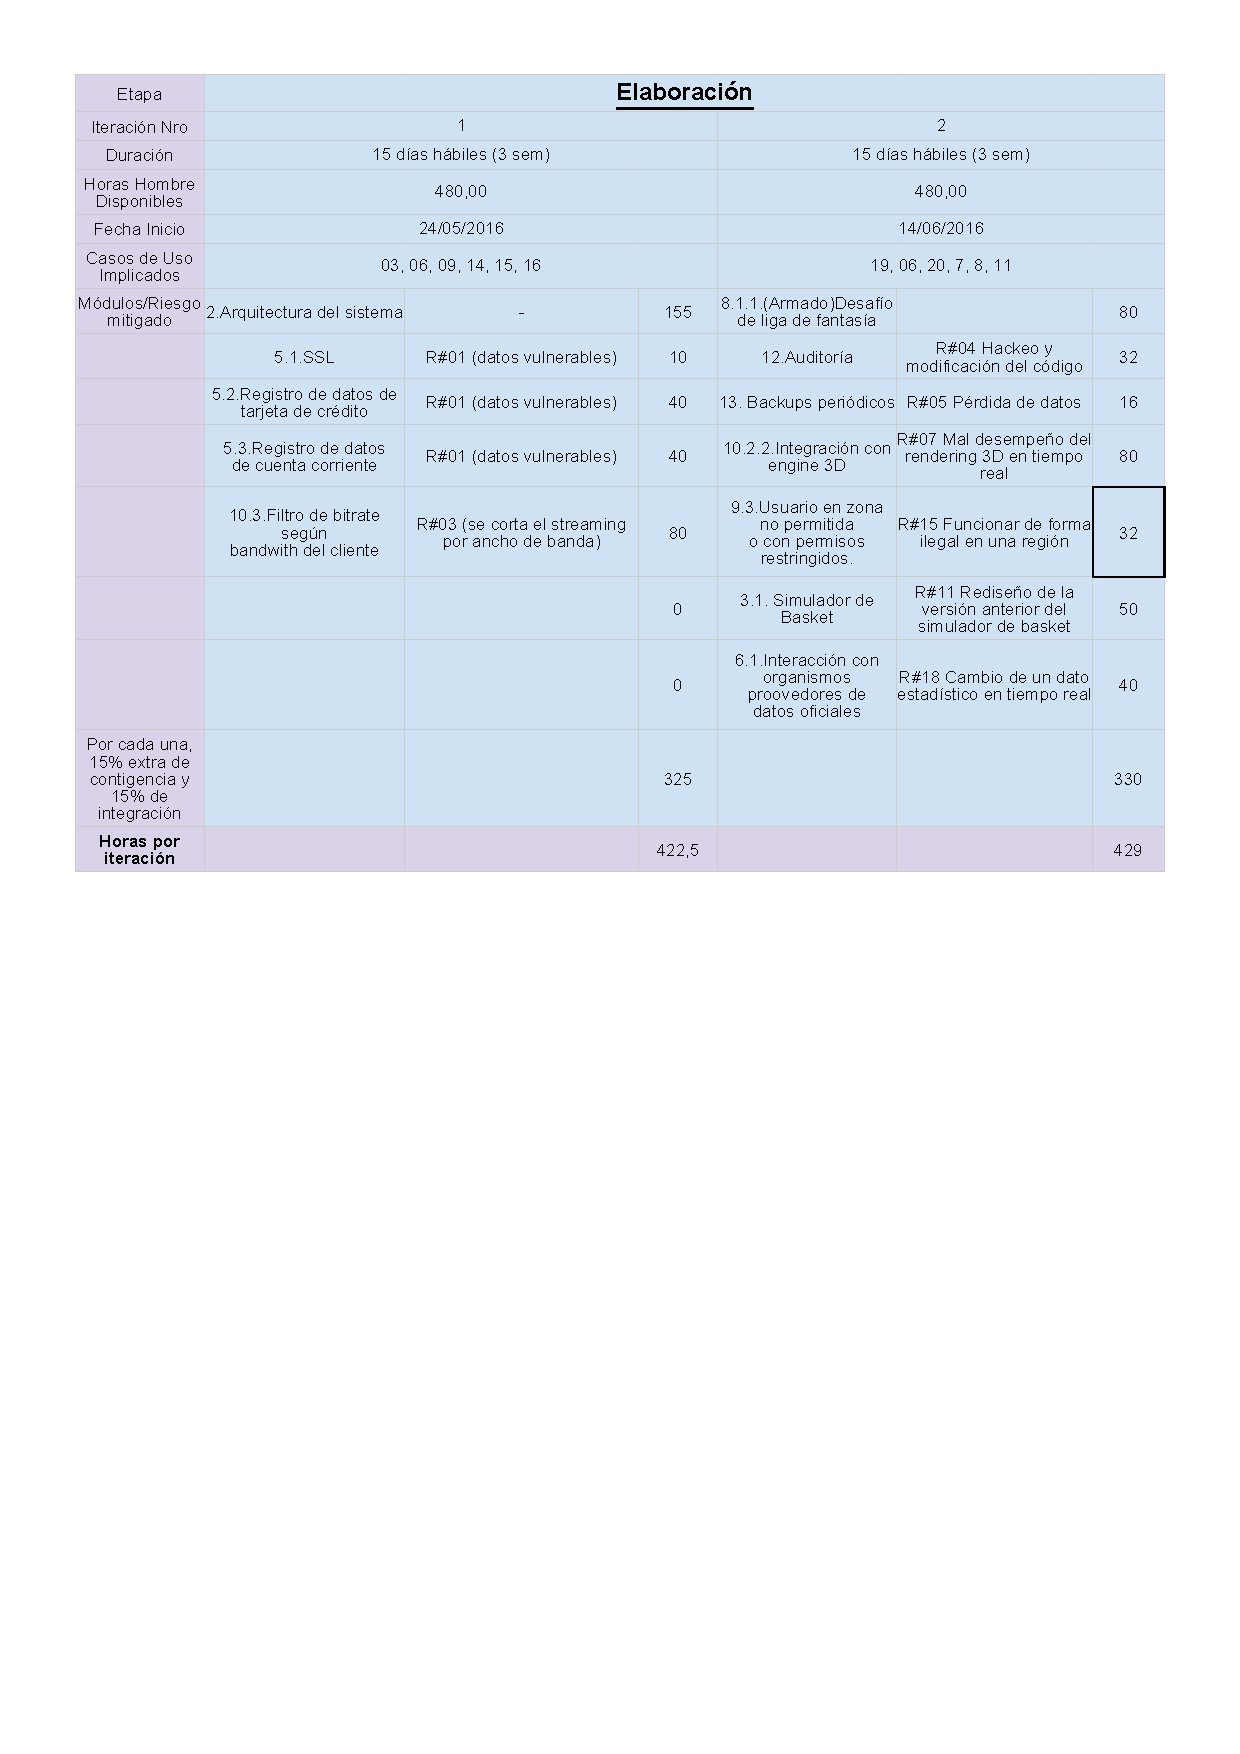
\includegraphics[scale=0.80]{imagenes/etapas-elaboracion.pdf}
   \caption{División de tareas en la etapa de elaboración}
\end{figure}

En la etapa de construcción se desarrollan los módulos y casos de uso faltantes faltantes de forma iterativa incremental. 

Finalmente en la etapa de transición se realizan tareas de mantenimiento.

\newpage
\begin{landscape}

\begin{figure}[h!]
   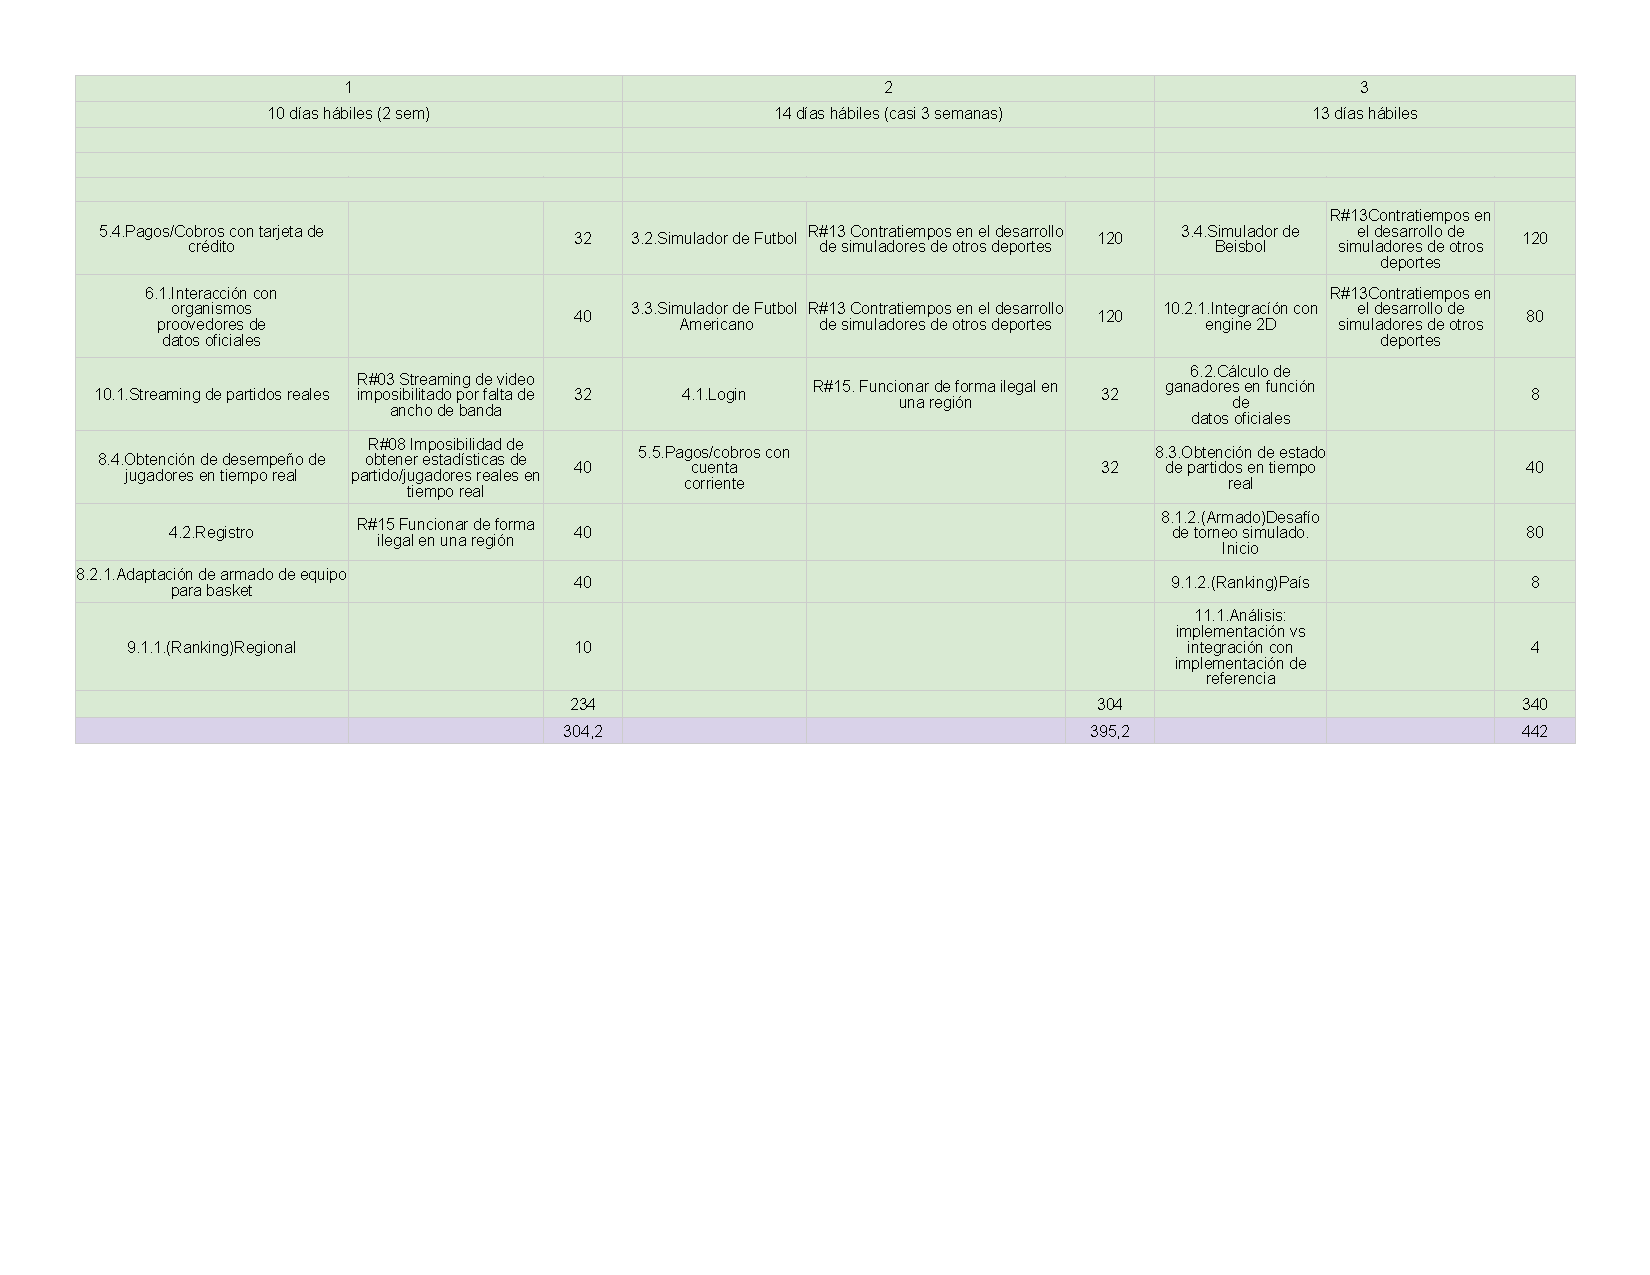
\includegraphics[scale=0.8]{imagenes/construccion123.pdf}
   \caption{División de tareas de las primeras 3 iteraciones de la etapa de 'Construcción'}
\end{figure}

\end{landscape}
\newpage

\newpage
\begin{landscape}

\begin{figure}[h!]
   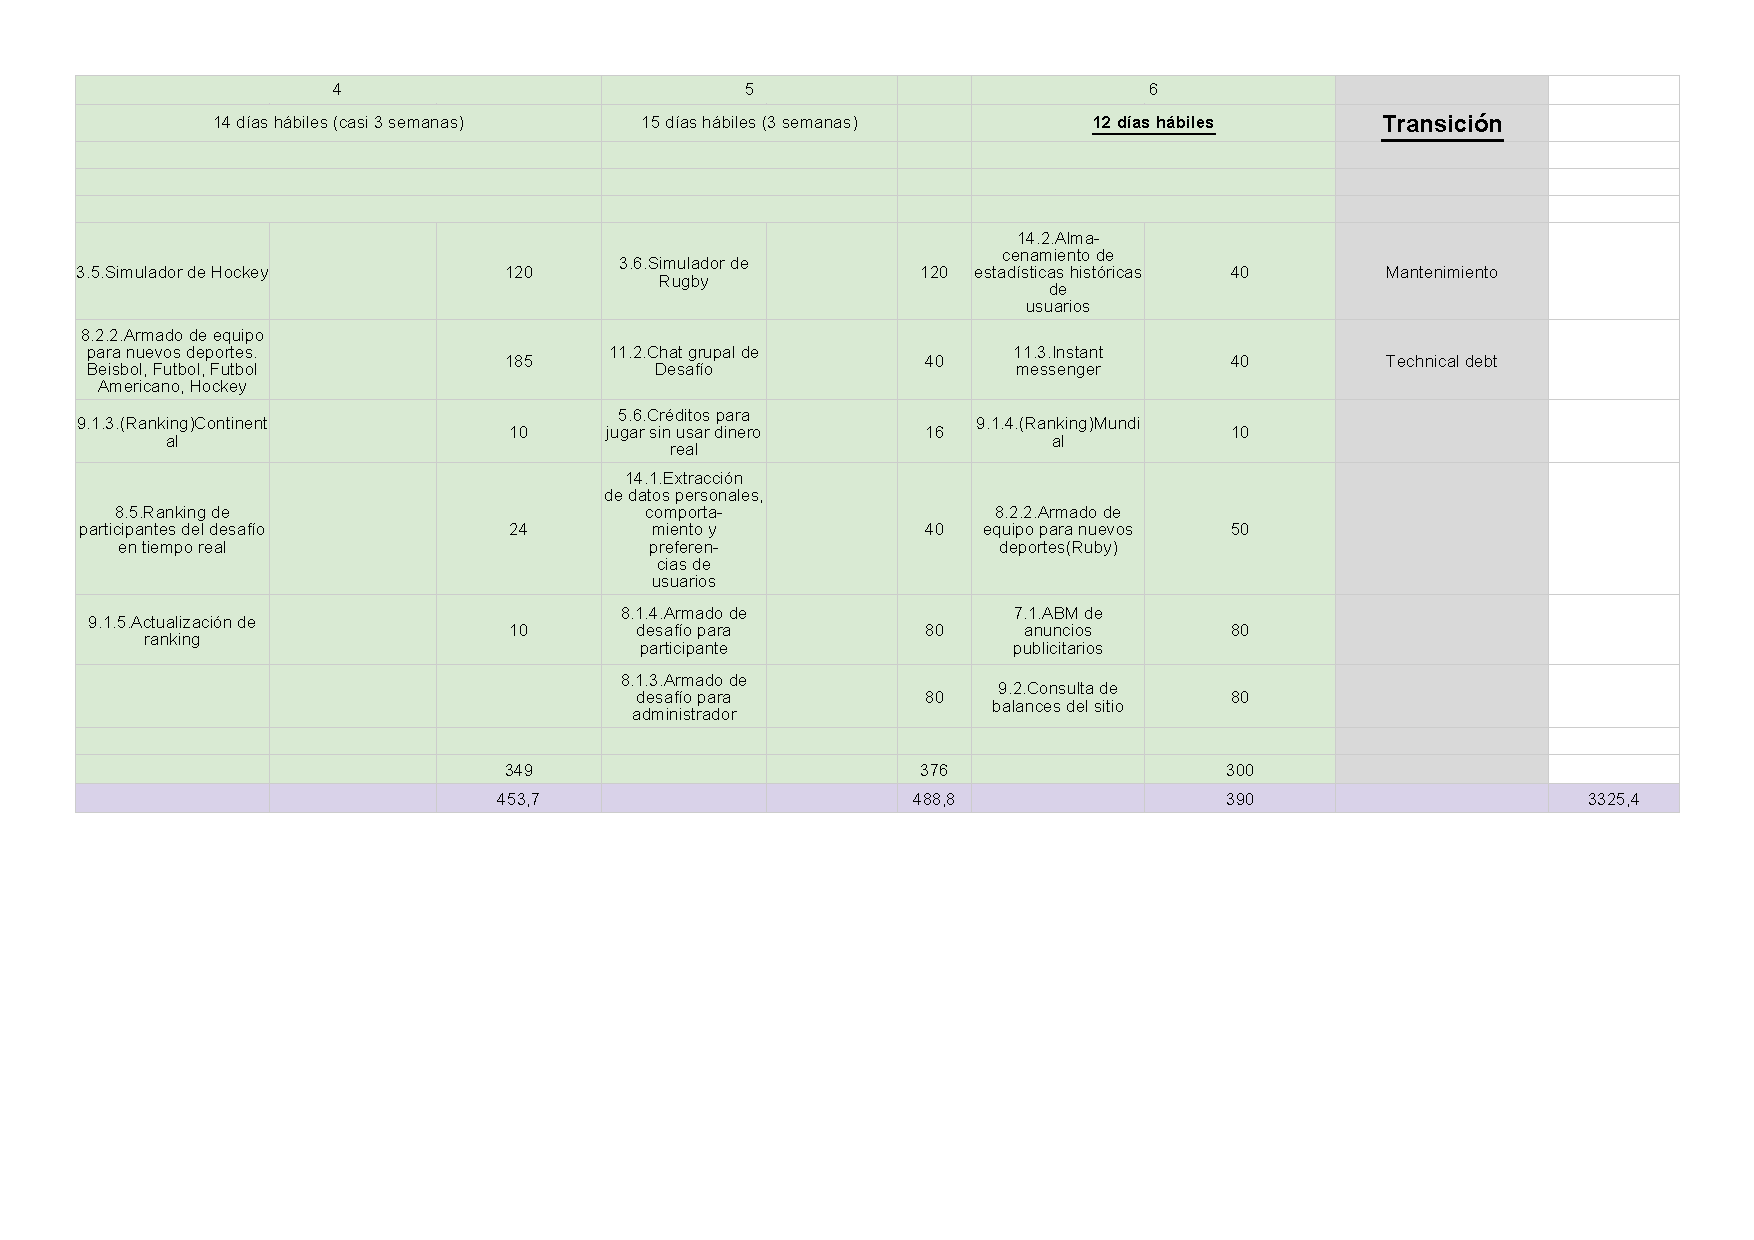
\includegraphics[scale=0.8]{imagenes/construccion-transicion.pdf}
   \caption{División de tareas de las últimas 3 iteraciones de la etapa de 'Construcción' y 'Transicion'}
\end{figure}

\end{landscape}
\newpage




% \subsection{Estimación de Módulos}
% A continuación se estima en horas hombre los módulos de nivel 1 y 2 del WBS. La estimación se basa en un grupo de trabajo de 4 recursos de 8 horas cada uno, 20 días por mes. Las horas hombre son las horas totales a consumir entre los 4 recursos sumados. Al final se realiza una sumarización de los números para estimar la duración total del proyecto.

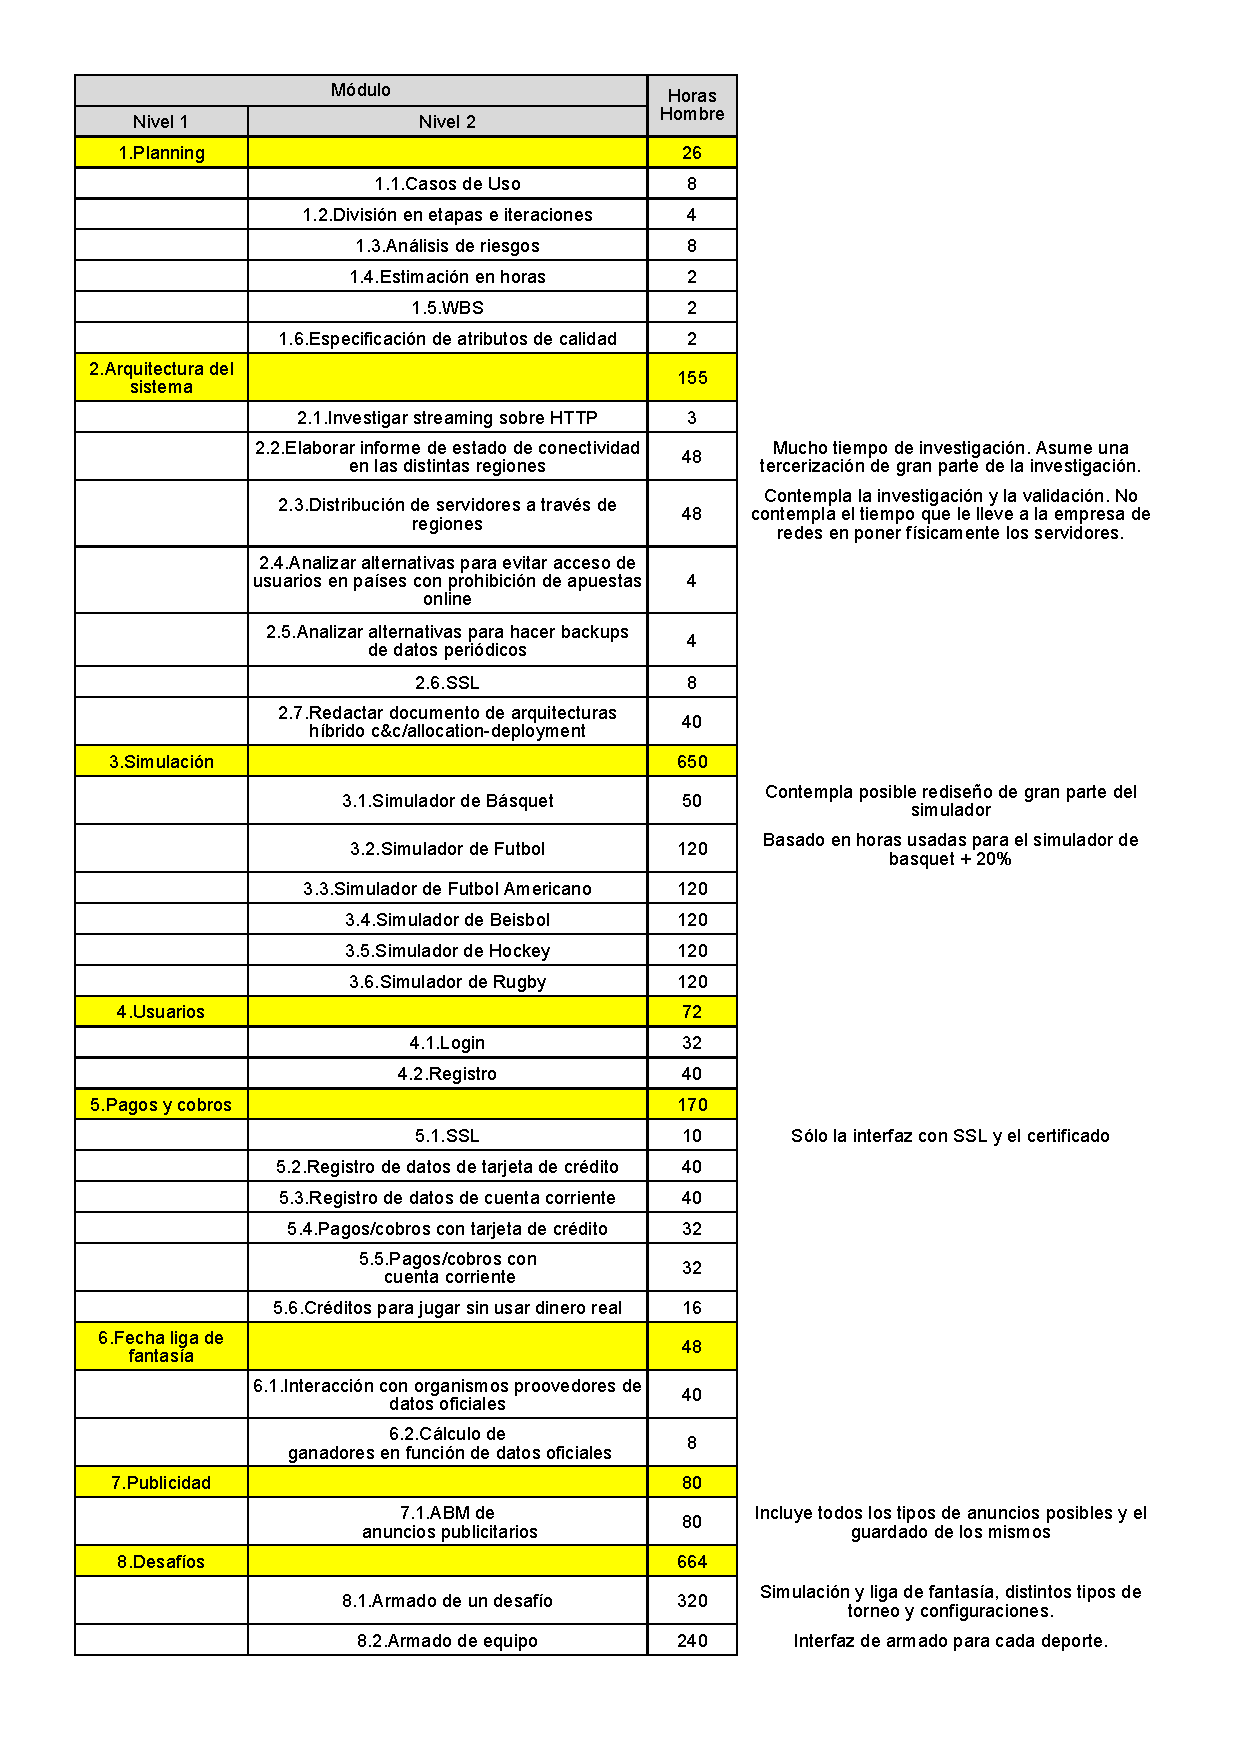
\includegraphics[width=\textwidth, page=1, clip, trim=20 0 20 30]{imagenes/estimacionModulos.pdf}

\newpage
\includegraphics[width=\textwidth, page=2, clip, trim=20 200 20 30]{imagenes/estimacionModulos.pdf}

Como puede observarse, el total estimado es bastante razonable para la magnitud del proyecto. Los tiempos podrían acelerarse si se contratara más gente y se tuviera un grupo de trabajo de 2 o 3 personas en cada módulo. Se estima que en 5 meses el proyecto debería estar funcionando, salvando las demoras que puedan causar los proveedores en responder y realizar su trabajo.
% \subsection{Division en etapas e iteraciones}
% En el proceso de elaboración se incluyen las tareas relacionadas con la arquitectura del sistema, y se genera una base ejecutable del código sobre la cual se pueda 
empezar a testear dicha arquitectura.

Al mismo tiempo se desarrollan los componentes con un rol central dentro de la arquitectura definida, y los módulos de los casos de uso con más riesgos
de alto impacto a nivel estructural, dejando cada una en una iteración diferente. La idea es construir la arquitectura de forma incremental. La opción a nivel arquitectura propuesta
en cada iteración debe ser compatible con la anterior, y al mismo tiempo solucionar el caso de uso actual.

\begin{figure}[h!]
   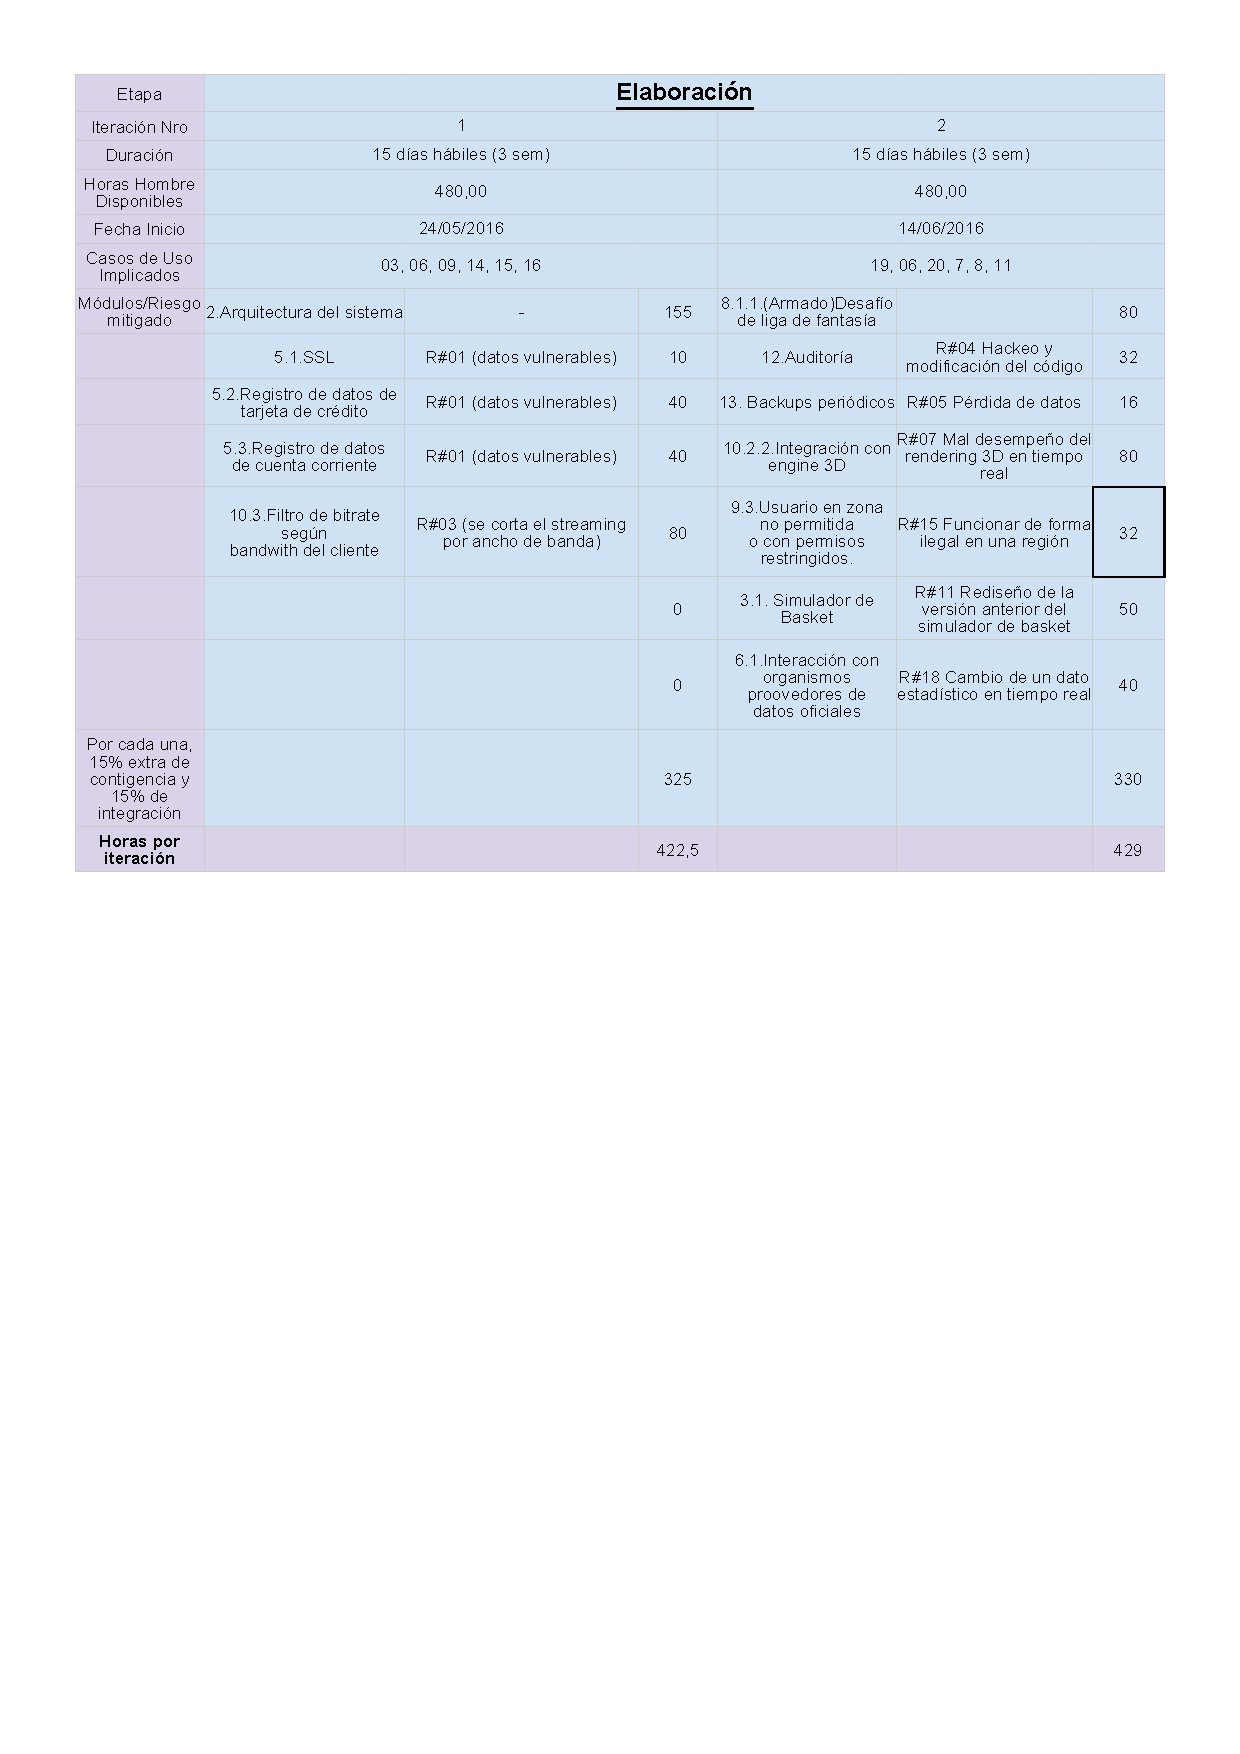
\includegraphics[scale=0.80]{imagenes/etapas-elaboracion.pdf}
   \caption{División de tareas en la etapa de elaboración}
\end{figure}

En la etapa de construcción se desarrollan los módulos y casos de uso faltantes faltantes de forma iterativa incremental. 

Finalmente en la etapa de transición se realizan tareas de mantenimiento.

\newpage
\begin{landscape}

\begin{figure}[h!]
   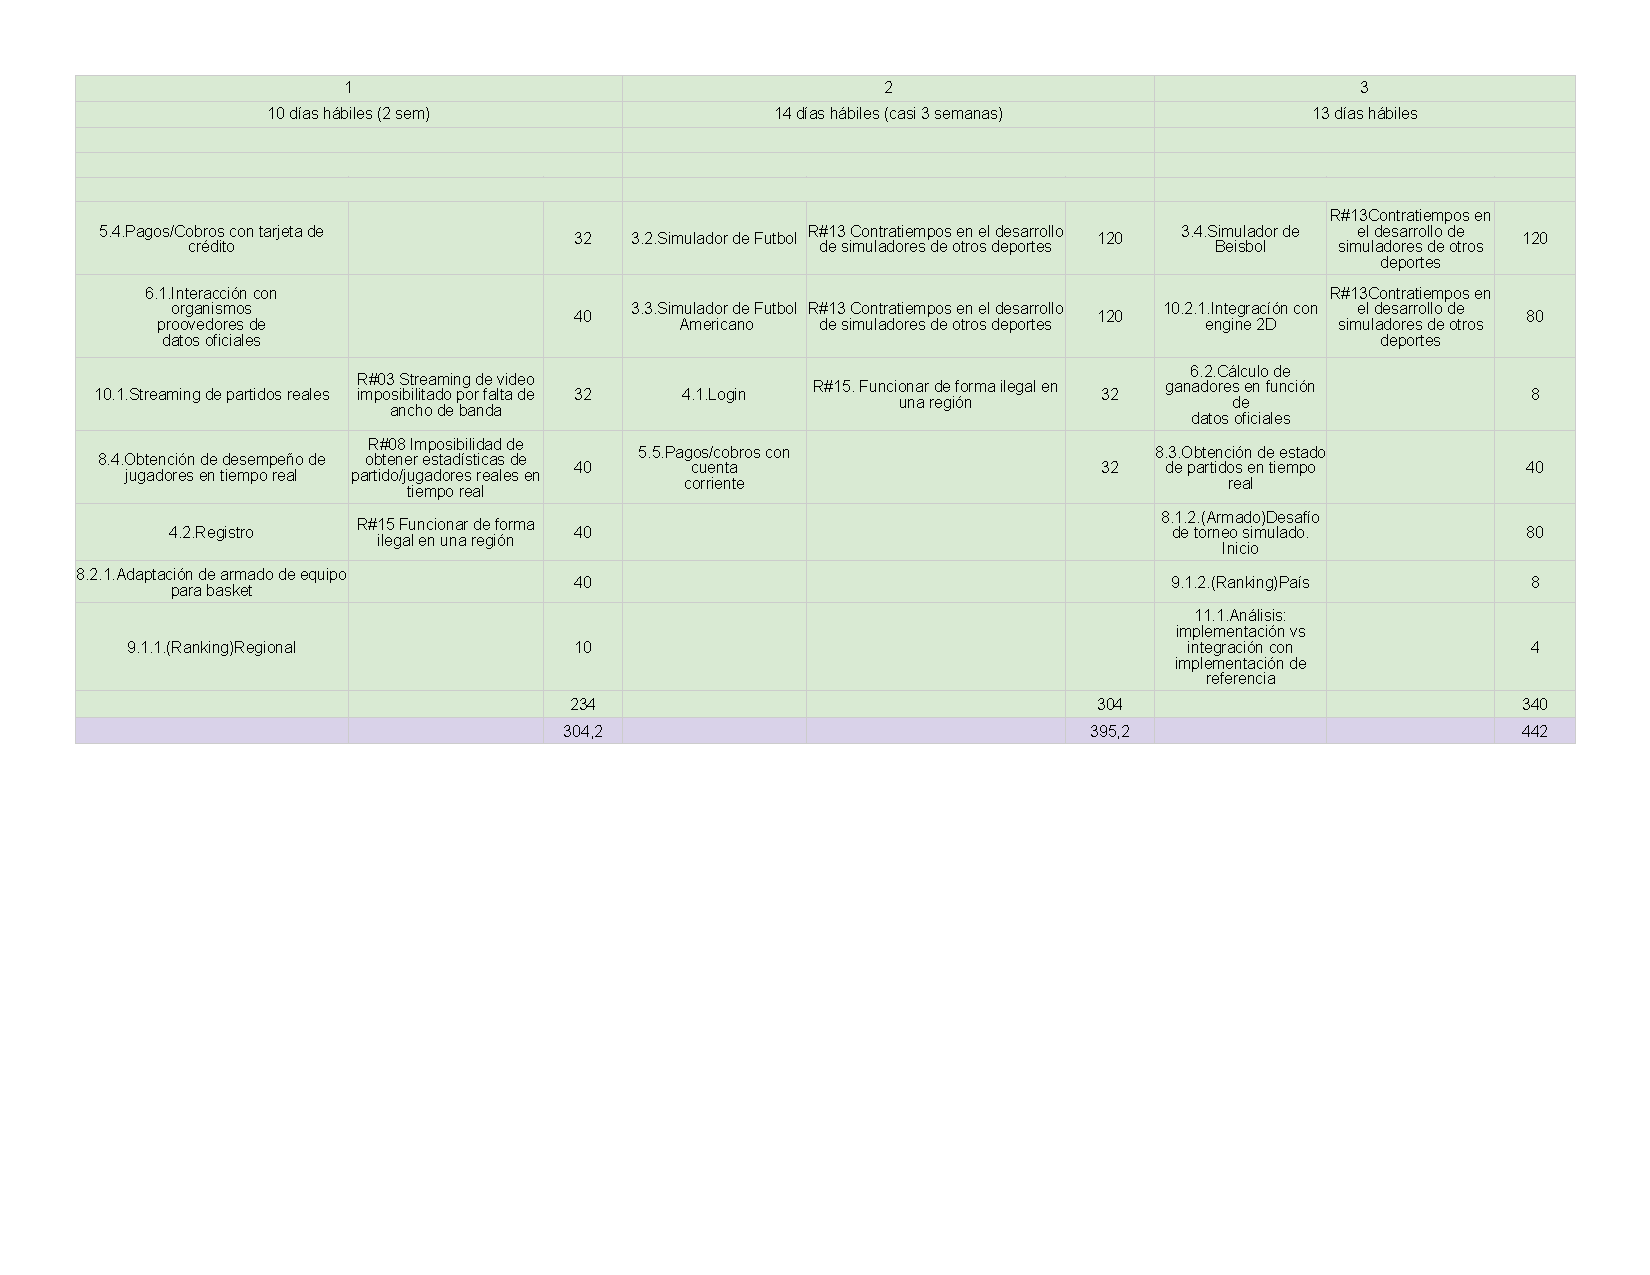
\includegraphics[scale=0.8]{imagenes/construccion123.pdf}
   \caption{División de tareas de las primeras 3 iteraciones de la etapa de 'Construcción'}
\end{figure}

\end{landscape}
\newpage

\newpage
\begin{landscape}

\begin{figure}[h!]
   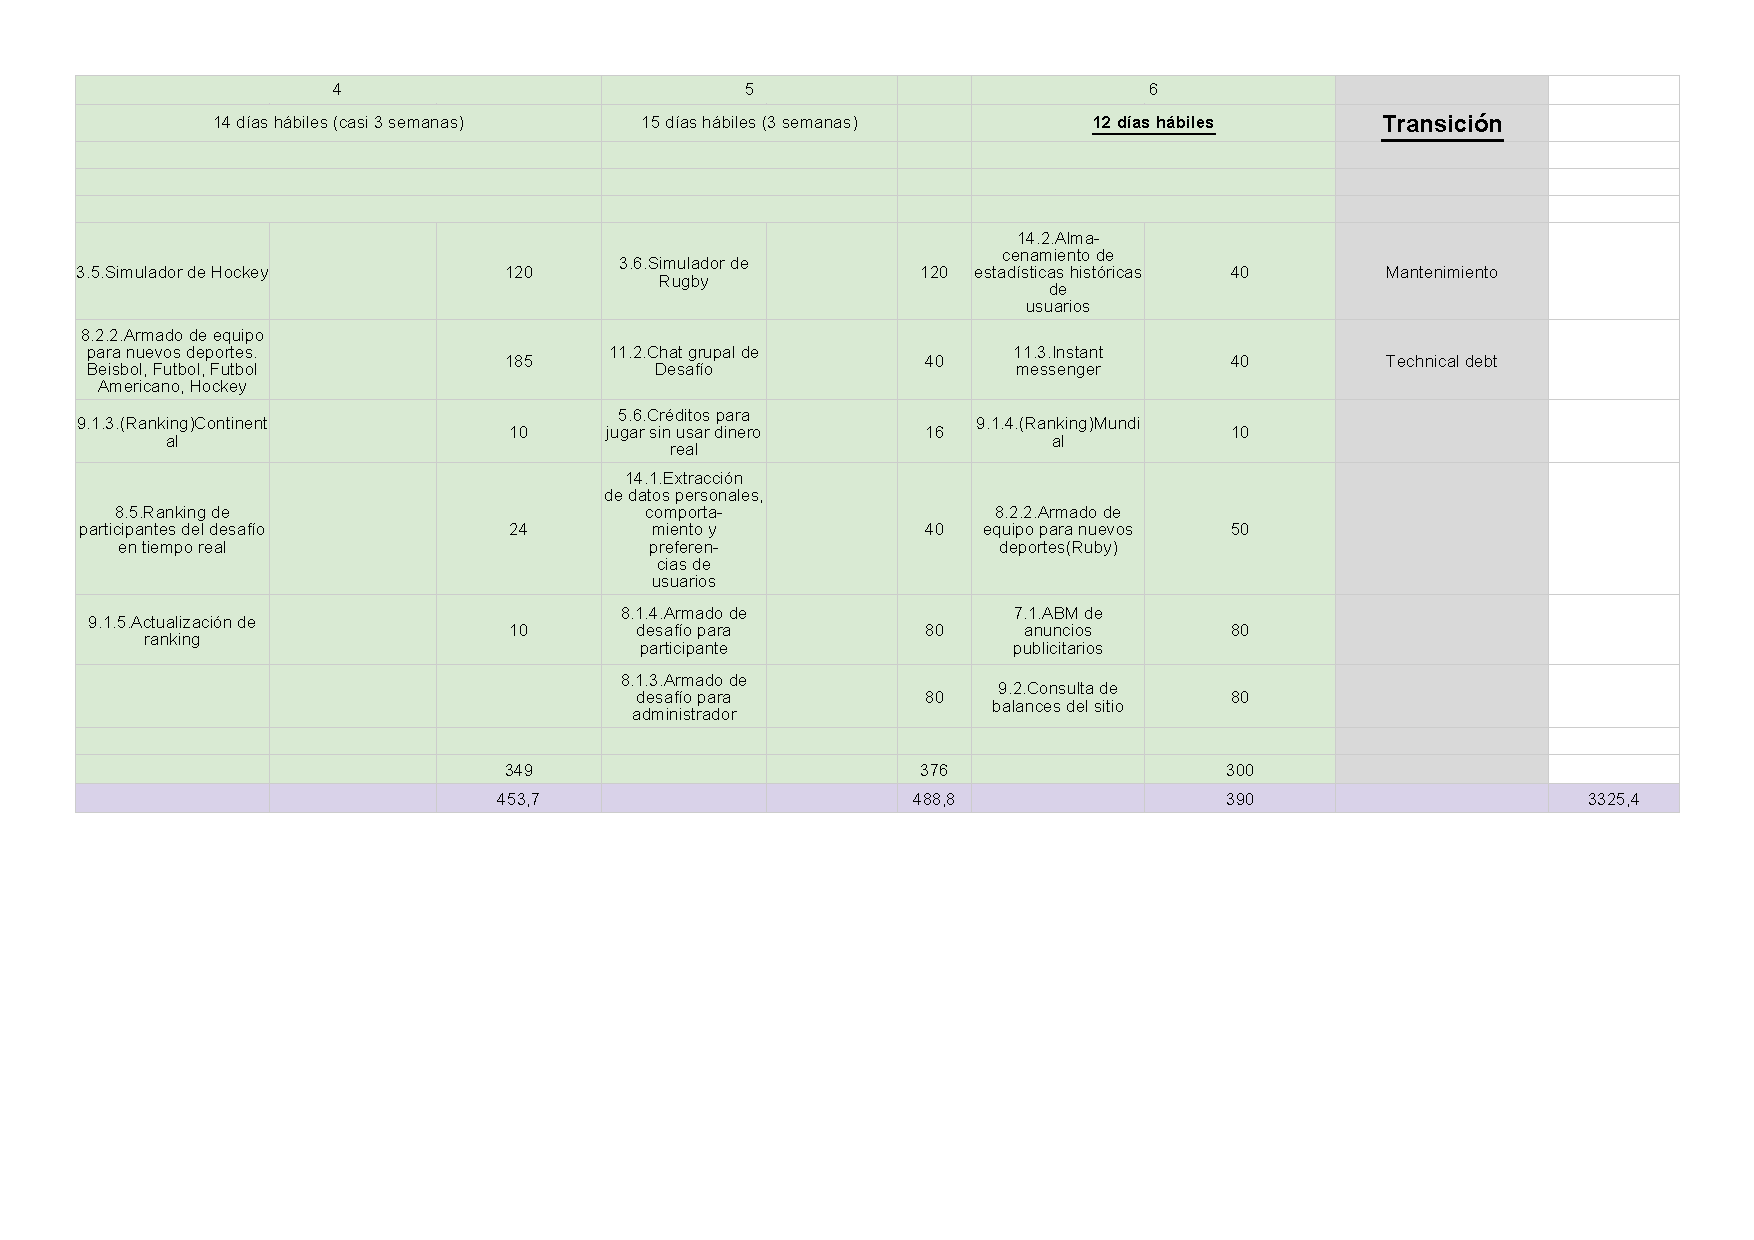
\includegraphics[scale=0.8]{imagenes/construccion-transicion.pdf}
   \caption{División de tareas de las últimas 3 iteraciones de la etapa de 'Construcción' y 'Transicion'}
\end{figure}

\end{landscape}
\newpage




% \section{Primer Entrega}
% No realizamos ninguna correción sobre la primer entrega, por lo que no la volvemos a presentar en esta
% entrega.
% \newpage
% \section{Atributos de calidad}
% En esta sección presentamos los escenarios de calidad que obtuvimos tras analizar los resultados del QAW.

\subsection{Atributos de disponibillidad}

\escenario
{Atributo de disponibilidad}
{El sistema debe estar andando todo el tiempo}
{Externa}
{Solicita acceso al sistema}
{Normal}
{Sistema}
{El sistema responde normalmente}
{Disponibilidad del 99,99\% (se puede caer aprox 1h en todo el año)}


~

\escenario
{Atributo de disponibilidad}
{Si falla un enlace regional, se redirige el tráfico a regiones cercanas de manera uniforme.}
{Servidor regional}
{No responde}
{Normal}
{Sistema}
{El sistema detecta la falla en el servidor regional y redirige el tráfico a las regiones más cercanas. La región entra en modo degradado. Se loguea la falla y se envía una notificación al técnico en redes}
{El servidor / enlace son reparados en menos de 24hs.}


~

\escenario
{Atributo de disponibilidad}
{Se produce una falla en una base de datos de un servidor}
{Interna}
{Falla en la base de datos de un servidor}
{Normal}
{Subsistema de almacenamiento y manejo de datos persistidos}
{El subsistema detecta y loguea la falla. El servidor originial continúa operando normalmente a través del uso de votación. La base de datos cambia a silencioso en el caso de ser la primera falla, y es reemplazada por una nueva instancia en caso de ser la segunda. Se envía una notificación al Data Base Manager.}
{Se garantiza disponibilidad a pesar de una falla en la base de datos el 99.99\% de las veces}

~

\escenario
{Atributo de disponibilidad}
{Se pierden datos de una base de datos de servidor}
{Interna}
{Pérdida de datos en una base de datos de servidor }
{Normal}
{Subsistema de almacenamiento y manejo de datos persistidos}
{El subsistema detecta y loguea la falla. El servidor recupera los datos ya que cuenta con una base redundante. La base de datos cambia a silencioso en el caso de ser la primera falla, y es reemplazada por una nueva instancia en caso de ser la segunda. Se envía una notificación al Data Base Manager.}
{Se mantienen los datos a pesar de una pérdida en una de las bases de datos el 99.99\% de las veces}

~

\escenario
{Atributo de disponibilidad}
{Se pierden los datos de todas las bases de datos de servidor}
{Interna o externa}
{Perdida de datos de todas las bases de datos de servidor}
{Normal}
{Subsistema de almacenamiento y manejo de datos persistidos}
{El subsistema detecta y loguea la falla. El servidor vuelve al último estado consistente de las últimas 4 horas, ya que realiza un backup cada esa cantidad de tiempo. Se restauran todas las bases. Se envía una notificación al Data Base Manager.}
{La probabilidad del escenario anterior es $<$ 0.00001\%. Las bases se restauran en un tiempo $< 4$ horas}

~

\escenario
{Atributo de disponibilidad}
{En cada región habrá varios servidores con una capacidad máxima de usuarios que puede atender, debido a limitaciones de hardware / conexión. Si nuevos usuarios se agregan y superan el 90\% de la capacidad, habrá que agregar un nuevo servidor y balancear la carga}
{Externa}
{Solicita acceso al sistema}
{A 1 pedido de alcanzar el límite de usuarios}
{Servidor regional}
{El servidor responde normalmente. Se incorpora un nuevo servidor a la red, y se aplica el balanceo de carga correspondiente}
{Se realiza la subdivisión de la región agregando un nuevo nodo en menos de 6 horas}

~

\escenario
{Atributo de disponibilidad}
{Enlaces congestionados durante streaming de partido real}
{Externa}
{Disminución de la capacidad de enlace durante streaming de partido real}
{Normal}
{Servidor regional}
{Se detecta el cambio de bitrate. Se realiza un downgrade de la calidad de video. El usuario continúa observando el partido de forma fluída, pero con menor calidad.}
{El streaming del video mantiene un rate constante de cuadros por segundo el 99.99\% de los casos}

~

\escenario
{Atributo de disponibilidad}
{Enlaces congestionados durante streaming de video de simulación}
{Externa}
{Disminución de la capacidad de enlace durante streaming de simulación}
{Normal}
{Servidor regional}
{Se detecta el cambio de ancho de banda del enlace. Se realiza un downgrade en el bitrate}
{El streaming de la simulación mantiene un rate constante de cuadros por segundo el 99.99\% de los casos}

~

\escenario
{Atributo de disponibilidad}
{Se caen enlaces de región durante transmisión de torneo continental o mundial}
{Externa}
{Caída de enlaces de región durante transmisión de torneo continental o mundial}
{Normal}
{Servidor regional}
{Se detecta la caída de los enlaces en la región. Se utiliza la topología de la conexión de regiones para triangular los paquetes y que lleguen a los usuarios.}
{El 99.99\% de las veces el usuario continúa viendo la transmisión del evento sin cortes abruptos, experimentando a lo sumo un cambio en la calidad del video}

\subsection{Atributos de performance}

\escenario
{Atributo de performance}
{Quiere que todo lo respectivo al manejo de dinero (depósitos y retiros de los participantes
via tarjeta de crédito o caja de ahorro) sea super seguro (no quiere papelones y que los
datos de las millones de tarjetas de los participantes aparezcan publicados en Reddit),
transparente y rápido. Que los datos queden resguardados y sólo haya que actualizarlos
esporádicamente.}
{usuario}
{depósito / retiro de dinero}
{operación normal}
{subsistema de pagos}
{el sistema realiza la operación satisfactoriamente}
{el sistema realiza la operación en menos de 15 segundos}

~

\escenario
{Atributo de performance}
{Propone un sistema de bitrate variable automático/manual de los streams de video para
que se pueda bajar la calidad de los videos en base al bandwidth detectado disponible del
usuario.}
{usuario}
{observa transmisión de partido}
{sistema degradado}
{sistema}
{se modifica calidad del video}
{se modifica la calidad del video en menos de 10 segundos}

~

\escenario
{Atributo de performance}
{Quiere que mientras sea posible se use el engine 3d de mayor calidad al 2d.}
{usuario}
{observa simulación de partido}
{sistema degradado}
{dispositivo móvil antiguo}
{se reemplaza engine 3d por 2d}
{antes de comenzar la reproducción de la simulación se reemplaza el engine 3d por 2d}


\subsection{Atributos de seguridad}

\escenario
{Atributo de seguridad}
{Atacante intenta robar datos de tarjetas de crédito o cuentas corrientes bancarias, pero el sistema lo impide}
{Atacante}
{Intenta robar datos de tarjetas de crédito o cuentas corrientes almacenados en servidores}
{Normal}
{Datos del sistema}
{Se detecta y se impide el ataque.}
{Se detecta y se impide el 99\% de los ataques.}

~

\escenario
{Atributo de seguridad}
{Atacante roba datos de tarjetas de crédito o cuentas corrientes bancarias, pero no puede descifrarlos}
{Atacante}
{Roba datos de tarjetas de crédito o cuentas corrientes almacenados en servidores}
{Normal}
{Datos del sistema}
{Se guardan los datos en un formato imposible de leer.}
{Toma más de 1000 años descifrar los datos.}

~

\escenario
{Atributo de seguridad}
{Atacante intercepta comunicación del sistema con el usuario.}
{Atacante}
{Interviene pasivamente una comunicación entre el usuario y el sistema}
{Normal}
{Comunicación del sistema}
{La comunicación está protegida por SSL, con lo cual el contenido de los paquetes es imposible de leer}
{Toma más de 1000 años descifrar los datos interceptados}


~

\escenario
{Atributo de seguridad}
{Atacante se hace pasar por el sistema para robarle datos al usuario.}
{Externa}
{Interviene activamente una comunicación entre el usuario y el sistema, tomando el rol del sistema}
{Normal}
{Comunicación del sistema}
{El sistema utiliza un mecanismo de autenticación del servidor mediante certificados y clave asimétrica. El browser alerta al usuario de que se han vulnerado los certificados SSL. Los paquetes obtenidos por el atacante están encriptados, por lo cual su contenido no puede determinarse}
{Los usuarios advertidos acerca del posible riesgo comienzan una nueva sesión segura el 99.99\% de las veces. En el caso de que el usuario envíe datos sin darse cuenta, toma más de 1000 años descifrar los datos interceptados}

~

\escenario
{Atributo de seguridad}
{Atacante modifica mensajes enviados entre el sistema y el usuario para forzar al sistema a realizar acciones no solicitadas por el usuario.}
{Externa}
{Interviene activamente una comunicación entre el usuario y el sistema, modificando mensajes capturados en el canal de comunicación}
{Normal}
{Comunicación del sistema}
{El sistema utiliza un mecanismo de verificación de integridad de los mensajes recibidos, tanto del lado del cliente como del servidor. El mecanismo de integridad viaja encriptado para evitar que sea modificado.}
{Toma más de 1000 años encontrar un mensaje que estando modificado tenga sentido y verifique la integridad.}

~

\escenario
{Atributo de seguridad}
{Un usuario logueado logra vulnerar el subsistema de pagos y cobros.}
{Usuario identificado}
{Vulnera el subsistema de pagos y cobros y genera movimientos de dinero a su favor}
{Normal}
{Subsistema de pagos y cobros}
{El sistema tiene un audit trail con el registro de todas las acciones realizadas por todos los usuarios logueados y revierte las operaciones realizadas por el usuario.}
{El 99.99\% de las veces el log tiene todos los datos necesarios para revertir las operaciones del usuario.}

~

\escenario
{Atributo de seguridad}
{Usuario no autorizado desea hacer uso de los datos recolectados por minería}
{Usuario sin privilegios de administrador}
{Intento de acceso a datos recolectados por minería}
{Normal}
{Sistema}
{El sistema loguea el intento de acceso. El sistema valida los permisos del usuario en el sistema y posteriormente niega el acceso}
{Los usuarios no autorizados no logran acceder a los datos el 99.99999\% de los casos}

~

\escenario
{Atributo de seguridad}
{Auditor verifica que el código de la simulación y cálculo de resultados de desafíos no se haya modificado}
{Auditor}
{Solicitud de hashes de auditoría para módulos de simulación y cálculo de resultados de desafíos}
{Normal}
{Sistema}
{Se otorgan los hashes correspondientes a ambos módulos}
{La coincidencia de los hashes obtenidos con los conservados con el auditor garantizan que el código no ha cambiado el 99.9999\% de los casos (muy baja probabilidad de colisiones en la función de hash)}

~

\escenario
{Atributo de seguridad}
{Usuario culpa al sistema de que no se le ha asignado el premio de un desafío en el que ha participado y ganado, pero no figura su lista de desafíos}
{Usuario}
{Acusación de premio no otorgado}
{Normal}
{Sistema}
{Se le muestra en base al audit trail del sistema el listado de todas las inscripciones a desafíos que realizó, quedando en evidencia que el usuario no se ha inscripto en dicho desafío}
{El audit trail mantiene una relación 1 a 1 con las operaciones del usuario en un 99.99\% respecto a las acciones del usuario del sistema. Es decir, no hay acciones que no estén logueadas y en el log aparecen únicamente acciones realizadas por dicho usuario}

~

\escenario
{Atributo de seguridad}
{Resolvedor de desafío de liga de fantasía obtiene un dato erróneo de una jugada provisto por el sistema externo que brinda resultados en real-time}
{Externa}
{Dato erróneo del sistema proveedor}
{Normal}
{Sistema}
{La resolución de una jugada en el minuto a minuto de un desafío de liga de fantasía es obtenida a partir de una votación, por lo que el resultado correcto es calculado}
{El proceso de votación obtiene el resultado correcto el 99.99\% de las veces}

\subsection{Atributos de modificabilidad}

\escenario
{Atributo de modificabilidad}
{Quiere ver estadísticas acerca del comportamiento de los participantes de todas las
temporadas (los más ganadores/perdedores en desafíos/dinero, los mejores/peores
equipos formado por participantes de diferentes caps, valores de caps de participantes,
rankings de regiones más ganadoras en desafíos/dinero, el modo de desafío más utilizado
por los participantes, etc...). Lo que está en paréntesis son sólo ejemplos. Quiere que la
mayor cantidad de datos que el sitio maneja pueda ser fácilmente minada por datos. Y
que esos datos pueda estar a cargo de administradores expertos para luego crear
desafíos acordes o otorgar créditos a participantes que califiquen.}
{administrador}
{agregar estadísticas acerca del comportamiento de los participantes}
{tiempo de ejecución}
{sistema}
{se agrega las nuevas estadísticas}
{se agregan las nuevas estadísticas en menos de una hora sin reiniciar el sistema}

~

\escenario
{Atributo de portabilidad}
{Debe de poder correr en la mayor cantidad de plataformas posibles, incluyendo móviles.}
{desarrollador}
{adaptar interfaz a una nueva plataforma}
{tiempo de diseño}
{interfaz de usuario}
{se adapta la interfaz a la nueva plataforma}
{se adaptan los cambios en menos de 50hs}

~

\escenario
{Atributo de modificabilidad}
{Quiere una interfaz similar al representante de empresas con derechos de televisación (Maxi) para controlar publicidades en las simulaciones y el sitio en general.}
{administrador}
{modificar publicidad}
{tiempo de ejecución}
{interfaz para el manejo de publicidades}
{se hace modificación de las publicidades}
{se muestran las nuevas publicidades en menos de 20 segundos}

~

\escenario
{Atributo de modificabilidad}
{Plantea necesidad de regionalizar la plataforma, debido a lo limitado y la mala calidad del
hardware/servidores disponibles para la plataforma en las regiones iniciales, sobre todo
teniendo en cuenta que los streams de video pasan por “dentro” del sistema. No se está
hablando de tercerizar el servicio a sitios como Vimeo o Youtube, sino que el tráfico pase
de alguna manera por los servidores del sitio. Los enlaces físicos/hardware subyacente
implica una cantidad de usuarios limitada / máxima por servidor}
{Interna}
{Incorporación una nueva región al sistema}
{normal}
{sistema}
{se incorpora una nueva región}
{el setup de la configuración se hace en menos de 5 horas}

~

\escenario
{Atributo de modificabilidad}
{También se quiere aumentar el caudal de redes sociales que se utilizan para “afectar” las estadísticas (no solo Twitter, sino incorporar Facebook,Google+, etc.)}
{desarrollador}
{incorporar una nueva red social al sistema}
{tiempo de diseño}
{sistema}
{se incorpora la nueva red social}
{se emplean menos de 40 hs}

~

\escenario
{Atributo de modificabilidad}
{Quiere que el énfasis se de en mejorar el módulo de simulación, para que sea lo más real
posible. Tiene contacto con asociaciones de jugadores e incluso jugadores, técnicos y
periodistas deportivos de diferentes deportes, para ayudar a mejorar el motor de
reglas/simulación. También tiene contacto con empresas de redes sociales/sentiment
analysis, para ayudar a interfacear con las mismas, y mejorar el módulo de
menciones/popularidad de los jugadores. El espíritu es que toda la simulación pueda irse
mejorando poco a poco hasta que represente lo mejor posible la realidad sin que sea un
dolor de cabeza introducir cambios.}
{sponsor, stakeholder}
{agregar nuevas reglas/acciones al motor de simulación}
{tiempo de diseño}
{motor de simulación}
{reglas/acciones nuevas agregadas sin efectos secundarios}
{se invierten menos de 10hs hombre}


\subsection{Atributos de usabilidad}

\escenario
{Atributo de usabilidad}
{Quiere poder que él y sus administradores de confianza puedan ver un dashboard en
tiempo real del estado de cuenta del sitio de cada una de las regiones y niveles (incluye locales, continentales, global, etc...) y de cualquier grupo de participantes.}
{administrador}
{ver estado de cuenta del sitio}
{tiempo de ejecución}
{sistema}
{el sistema provee un dashboard con el estado de cuenta del sitio de cada una de las regiones}
{el administrador es capaz de administrar / comprender la información suministrada en menos de 5 minutos}

~

\escenario
{Atributo de usabilidad}
{Aunque no es su responsabilidad, le interesa que la interfaz gráfica de usuarios tenga la
calidad de un “juego”, sobre toda al momento de ver a los jugadores, las jugadas de los
técnicos, colocar el nombre y logo del equipo del participante, etc... con animaciones y
efectos especiales con aceleración gráfica (blurs, iluminación dinámica, depth of field, etc).}
{usuario}
{el usuario desea administrar su equipo}
{operación normal}
{Interfaz web / Móvil}
{se muestra una interfaz gráfica llena de animaciones en donde el usuario puede administrar su equipo }
{el test de usabilidad supera el 95\% de satisfacción}

~

\escenario
{Atributo de usabilidad}
{Usabilidad del subsistema controlador de publicidades en las simulaciones y en el sitio}
{Usuario administrador de publicidades}
{Desea minimizar el impacto de sus errores al configurar publicidades}
{Runtime}
{Sistema}
{Se provee un botón de cancelación para volver a la configuración anterior}
{Los cambios realizados se vuelven atrás y las publicidades no cambian.}

~

\escenario
{Atributo de usabilidad}
{Usabilidad del subsistema controlador de publicidades en las simulaciones y en el sitio}
{Usuario administrador de publicidades}
{Desea estar seguro de dónde se muestra en el sistema la publicidad que está modificando}
{Runtime}
{Sistema}
{Se provee una previsualización de cada publicidad, ubicada en el entorno gráfico que corresponde, acompañada de un texto descriptivo.}
{Durante 1 hora se le enseña a dos personas a usar la interfaz de ABM de publicidades y luego se les solicita hacer cambios en todas las publicidades. Modificarán correctamente al menos el 80\%.}

~

\escenario
{Atributo de usabilidad}
{Usabilidad del subsistema controlador de publicidades en las simulaciones y en el sitio}
{Usuario administrador de publicidades}
{Desea insertar la misma publicidad en muchos lugares del sistema de forma eficiente}
{Runtime}
{Sistema}
{Se provee una funcionalidad especial para cargar una publicidad eligiendo múltiples sitios.}
{Toma a lo sumo 3 clicks adicionales cargar una publicidad en muchos sitios que cargarla en un único sitio (además de todos los clicks necesarios para seleccionar los distintos sitios) (suponiendo que no se cometen errores en la selección de sitios).}

~

\escenario
{Atributo de usabilidad}
{Usabilidad del subsistema de pagos y cobros}
{Usuario}
{Desea estar tranquilo de que ingresar en el sistema su número de tarjeta de crédito o cuenta corriente es seguro.}
{Runtime}
{Sistema}
{Se muestran los nombres de las autoridades que auditaron la seguridad del sistema y los documentos que lo prueban.}
{En menos de 5 minutos el usuario se anima a ingresar sus datos.	}


% \escenario
% {Atributo de auditabilidad}
% {}
% {administrador}
% {buscar operaciones hechas con tarjeta de crédito}
% {operación normal}
% {sistema}
% {se muestra la operación buscada}
% {cada vez que se realiza una operación con tarjeta de crédito se guarda quién la hizo, en qué momento, en qué ip y qué monto se acreditó / retiro}














































% \section{Arquitectura}
% En esta sección presentamos la arquitectura que proponemos para cumplir con los atributos de calidad
ya planteados.

\subsection{Diagrama de nivel 0}
\begin{figure}[H]
  \centering
  \includegraphics[width=\textwidth]{imagenes/Nivel0.png}
  \caption{Diagrama de Arquitectura de nivel 0.}
\end{figure}
\newpage

\subsection{Diagrama de nivel 1}
\begin{figure}[H]
  \centering
  \includegraphics[width=\textwidth]{imagenes/Nivel1.png}
  \caption{Diagrama de Arquitectura de nivel 1.}
\end{figure}

El sistema se compone de N de estas instancias. Cada una representa el software que corre en un servidor. N representa la cantidad de regiones (mínima unidad geográfica) en donde corre el sistema. Cada instancia está deployada en un servidor independiente, ubicado en dicha región. Cada uno de estos servidores tiene una réplica que corre en modo shadow por si el servidor primario falla.
El sistema se compone también del conjunto de componentes que corre en los dispositivos de los usuarios.

Cada servidor almacena datos locales a su región. Las estadísticas que almacena, la información de desafíos, la información de sus usuarios son en su gran mayoría regionales, con la excepción
de que dicho servidor esté siendo utilizando para algún desafío como nodo intermedio en el árbol de jerarquía de desafíos extra-regionales. (Ver documento jeraraquía global). En ese caso,
almacena y propaga los datos del desafío que está simulando.

La comunicación entre el cliente y el servidor se realiza de 4 formas diferentes: Streaming de partido real, obtención de datos para rendering de simulación, realizar una compra de fichas
para apostar o extracción de dinero y finalmente pedidos de consulta web comunes como ser: registración, login, consulta de ranking, creación de equipo, participación de desafío, etc. Llamamos
'pedido general' a esta última categoría. Cada una de estas 4 formas de comunicación utiliza un conector distinto ya que necesitan satisfacer diferentes requerimientos.
Estos conectores tienen un estilo call-return para poner énfasis en que la comunicación es sincrónica: Un usuario hace un pedido de streaming. A partir de ese momento se inicia una
sesión entre el servidor y el usuario para mandar un flujo de datos a través del canal de comunicación que dura hasta que finaliza la conexión.

El subsistema de desafíos maneja tanto las simulaciones como las ligas de fantasía.

'Currification' tiene un acuerdo con las empresas televisivas proveedoras de transmisiones, mediante la cual permite crear enlaces para satisfacer los pedidos de los usuarios para ver
partidos televisados. El manejador de pedidos recibe los datos de cada transimisión a través de un pipe, y resuelve a través de un mapping sesiones de usuarios vs transmisiones para
saber qué transmisiones debe enviarle a cada usuario. Una situación análoga sucede con las simulaciones.

Los stakeholders pueden agregar publicidades a través de una interfaz gráfica intuitiva y simple. Esta les permite decidir en qué lugar mostrarán cada publicidad: UI de la web,
rendering de simulaciones o streaming de partidos. Por este motivo, el subsistema de publicidad rutea las nuevas publicidades a los subsistemas correspondientes.

Los controles de auditoría se hacen sobre los subsistemas de pagos y cobros (para corroborar que no haya movimientos irregulares de dinero), y sobre el subsistema de simulación de
desafíos, verificando que el hash del código de simulación no haya sido modificado.

La autenticación y restricción al sitio por parte de los usuarios se realiza a partir de reglas: Algunas direcciones de IP están restringidas. Correspondientes a aquellas zonas en donde
están prohibidas las apuestas web. Por otro lado, cuando un usuario asocia una tarjeta a su cuenta el sistema verifica que la tarjeta sea local a la región a la cual se encuentra.
Finalmente, cuando un usuario quiere realizar una compra utilizando una tarjeta, esta última debe coincidir con aquella que ha sido registrada previamente.


\newpage

\subsection{Jerarquia Virtual}
\begin{figure}[H]
  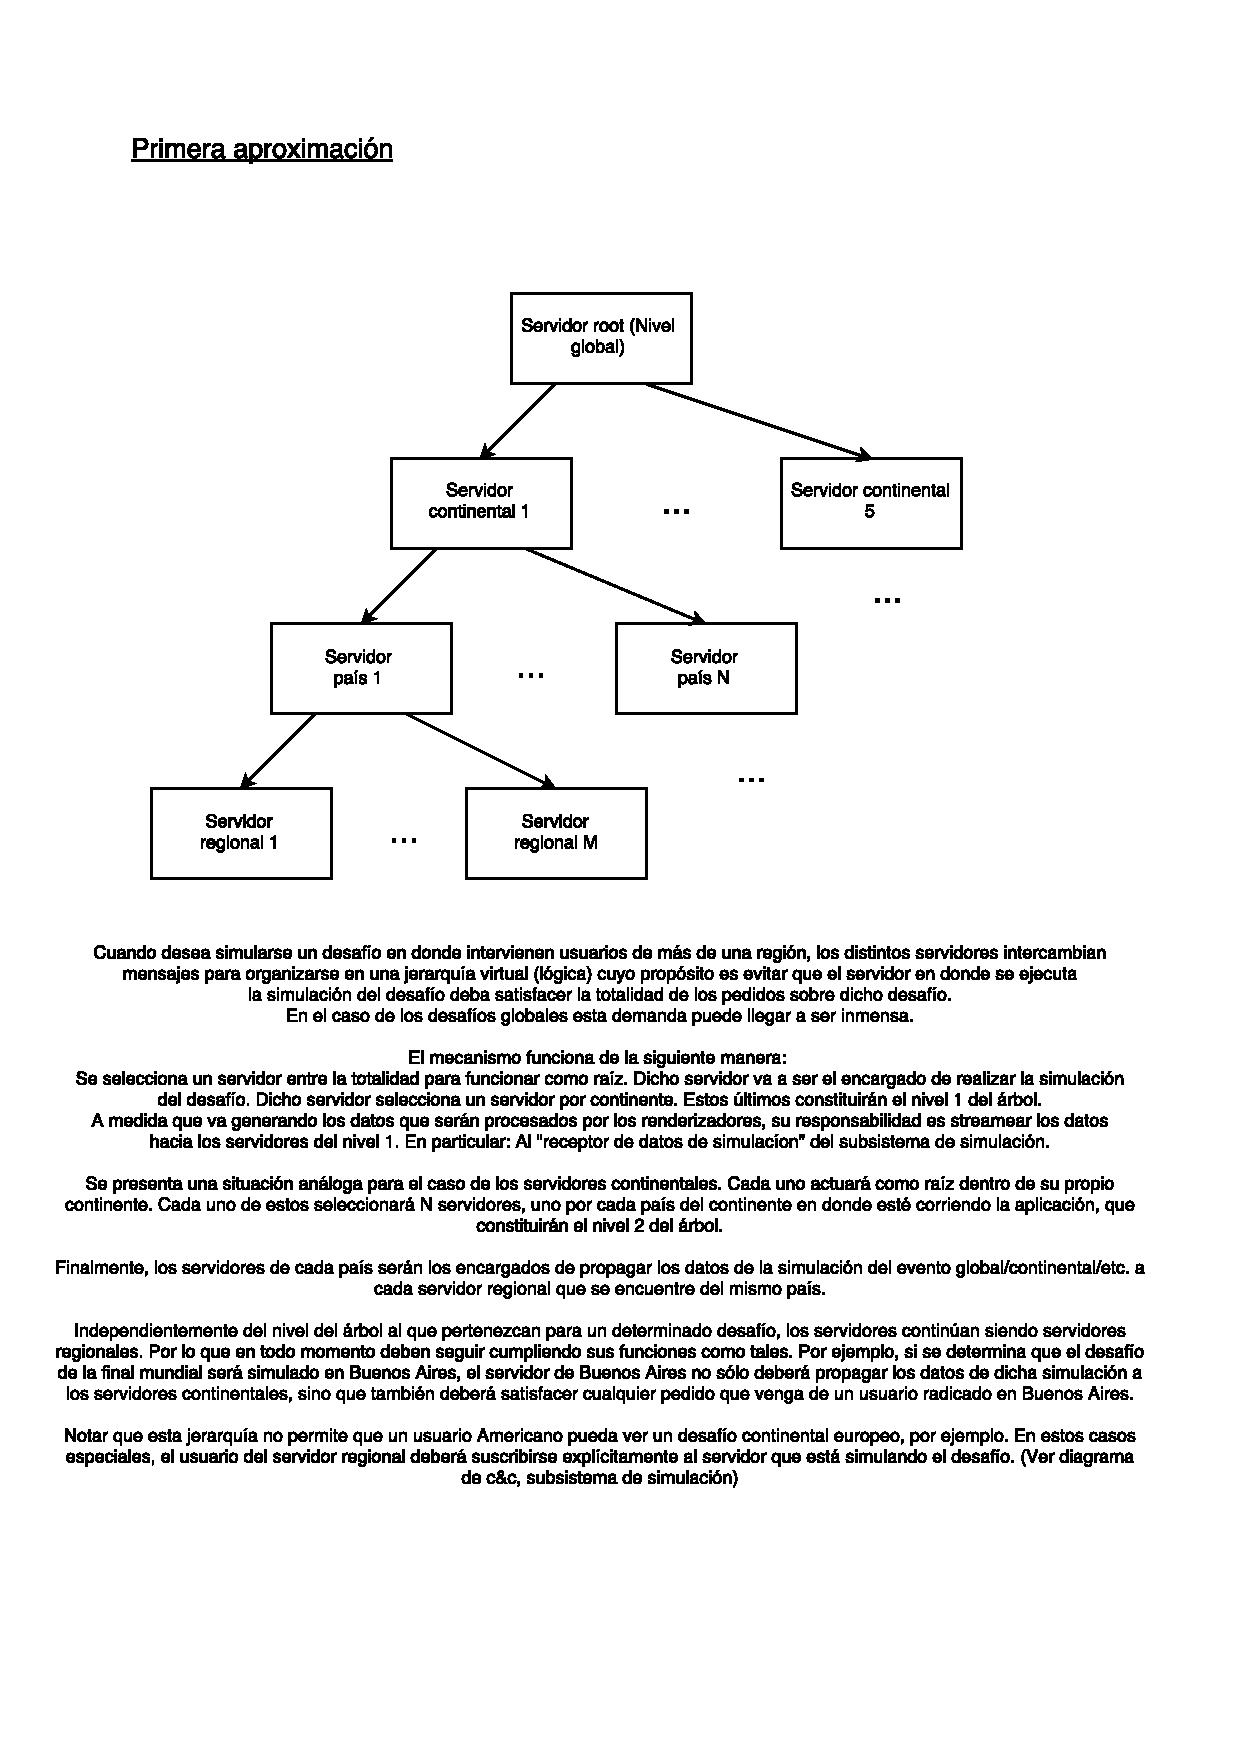
\includegraphics[width=\textwidth, page=1, clip, trim=20 0 20 110]{imagenes/jerarquia-global.pdf}
\end{figure}
\newpage
\begin{figure}[H]
  \includegraphics[width=\textwidth, page=2, clip, trim=20 20 20 10]{imagenes/jerarquia-global.pdf}
\end{figure}

\begin{figure}[H]
  \centering
  \includegraphics[width=\textwidth]{imagenes/nivel1-simulaciones.png}
\end{figure}

\newpage

\subsection{Subsistema de Desafios}
\begin{figure}[H]
  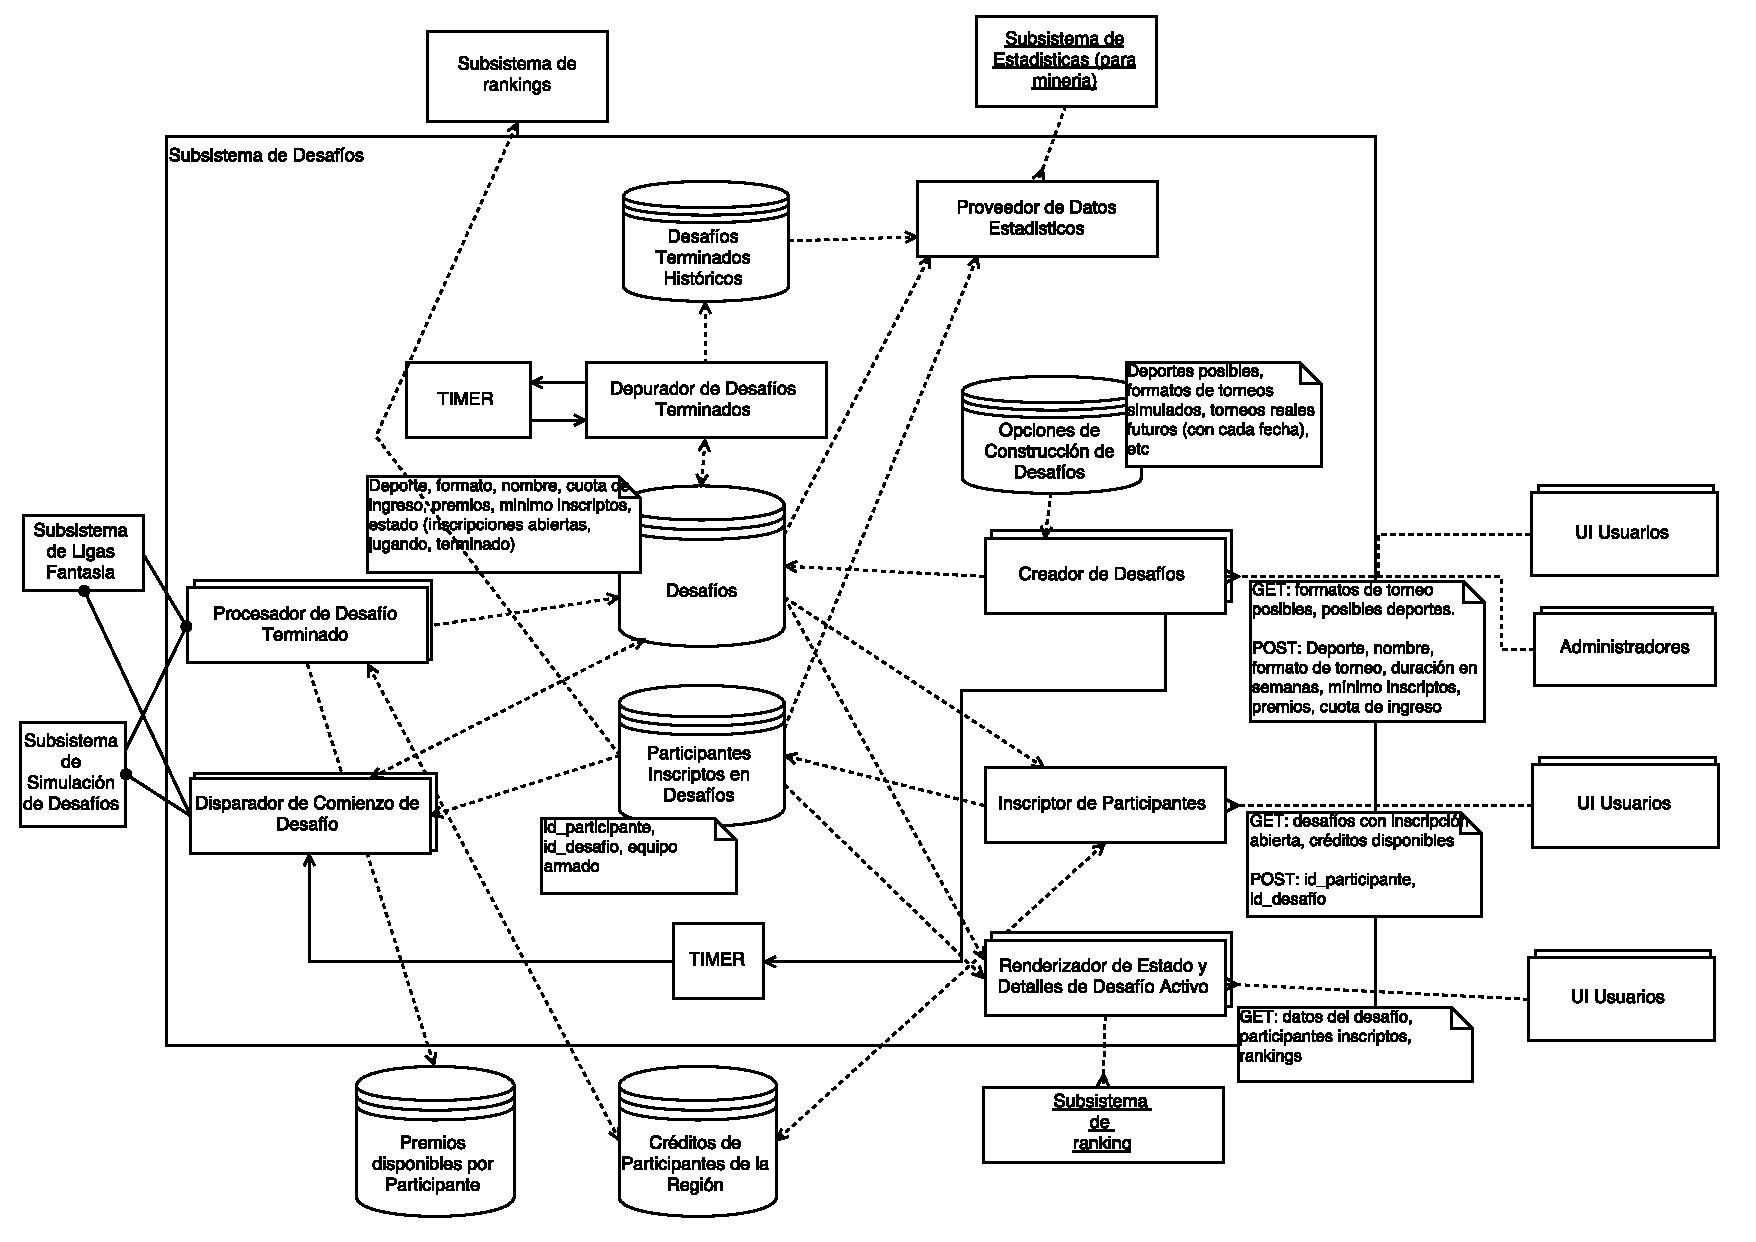
\includegraphics[width=1.1\textwidth, page=1, clip, trim=10 0 10 0]{imagenes/Subs-desafios.pdf}
  \caption{Subsistema de Desafios.}
\end{figure}
% \newpage
El subsistema de desafíos se encarga de crear desafíos, inscribir participantes, iniciar desafios en el momento indicado, proveer detalles y estado de cada desafio a los usuarios.
Cuando un desaífo comienza se encarga de informar al subsistema de simulación o liga de fantasia seúgn corresponda. Además se encarga de cobrar créditos de inscripción y de pagar premios (tanto en créditos como premios especiales, que luego los usuarios podrán cambiar por el premio real en dinero o lo que corresponda. También provee una interfaz de consulta de estadísticas de desafios.\\

\begin{itemize}
\item Desafíos Terminados: Los desafíos finalizados durante la última semana van a tener más solicitudes de consulta de estado. Es por esto que esos desafíos se mantienen
en el repositorio principal de desafíos con redundancia activa para mejorar la disponibilidad y la performance. Pasados los 7 días de finalizado, un proceso que ejecuta una vez por día se encarga de depurar el repositorio principal para mejorar la performance de las búsquedas, asumiendo que esos desafíos serán consultados con menos frecuencia.

\item Creador de Desafíos: Devuelve todas las opciones posibles para construir un desafío (tanto para modo simulado como para modo liga de fantasía). Luego recibe la configuración elegida y crea el desafío. Se almacena en un repositorio local que luego se propaga a todas las réplicas regionales.

\item Inscripción de participantes: Muestra una lista con todos los desafíos por cada deporte (tanto simulados como liga de fantsía) que aún estén con la inscripcion abierta (aún no comenzaron ajugarse). Por cada uno muestra el valor en creditos para ingresar. Luego se inscribe un participante (siempre y cuando ls créditos le alcancen). Para mejorar la performance y disponibilidad (muchos podíran intentar inscribirse a la vez), luego de hacer el checkeo se guardan en una caché todos los pedidos de  inscripcion que luego se van persistiendo por procesos dedicados.

\item Renderizador de estado y detalles: Devuelve el estado de un desafio especifico (si está abierto a inscripciones, si se esta jugando o si está terminado) asi como también la cuenta regresiva para que empiece el desafio (y se cierren inscripciones) y todos los detalles asociados (premios, cuota de inscripción, tipo de desafío, formato de torneo o fechas que se juegan, etc.), y el ranking, si corresponde. Internamente se utiliza una caché. Cada pedido que llega se guarda en un repositorio y se solicitan los datos a un manager de cache (que se crea en el momento que se necesita) y a un proceso que busca los datos en los repositorios persistentes (tambéin se crea cuando se necesita). Si el dato llega de la caché, se mata al proceso que  fue a disco (y tambien se mata al proceso de la caché). En cambio si no estaba en la caché, el dato llegaár del disco (y ahí tambéin se guarda en la caché para soportar eficentemente un período corto de muchos pedidos de detales del mismo desafio. Un proceso se ejecuta cada 1 minuto y borra los datos de caché que tengan más de un minuto de antigüedad. Dado que los datos no deben mostrarse en tiempo real, este mcanismo mejora la disponibildad y la performance de respuesta a muchas solicitudes de detalles de un desafío popular.
\end{itemize}

\begin{figure}[H]
  \includegraphics[width=\textwidth, page=3, clip, trim=20 0 20 30]{imagenes/Subs-desafios.pdf}
  \caption{Zoom en Procesador Desafio Terminado y Creador de Desafios}
\end{figure}

\begin{figure}[H]
  \includegraphics[width=\textwidth, page=4, clip, trim=20 0 20 0]{imagenes/Subs-desafios.pdf}
  \caption{Zoom en Inscriptor de Participantes y Renderizador de Estados y Detalles Desafio Activo}
\end{figure}

\newpage

\subsection{Subsistema de Simulacion}
\begin{figure}[H]
  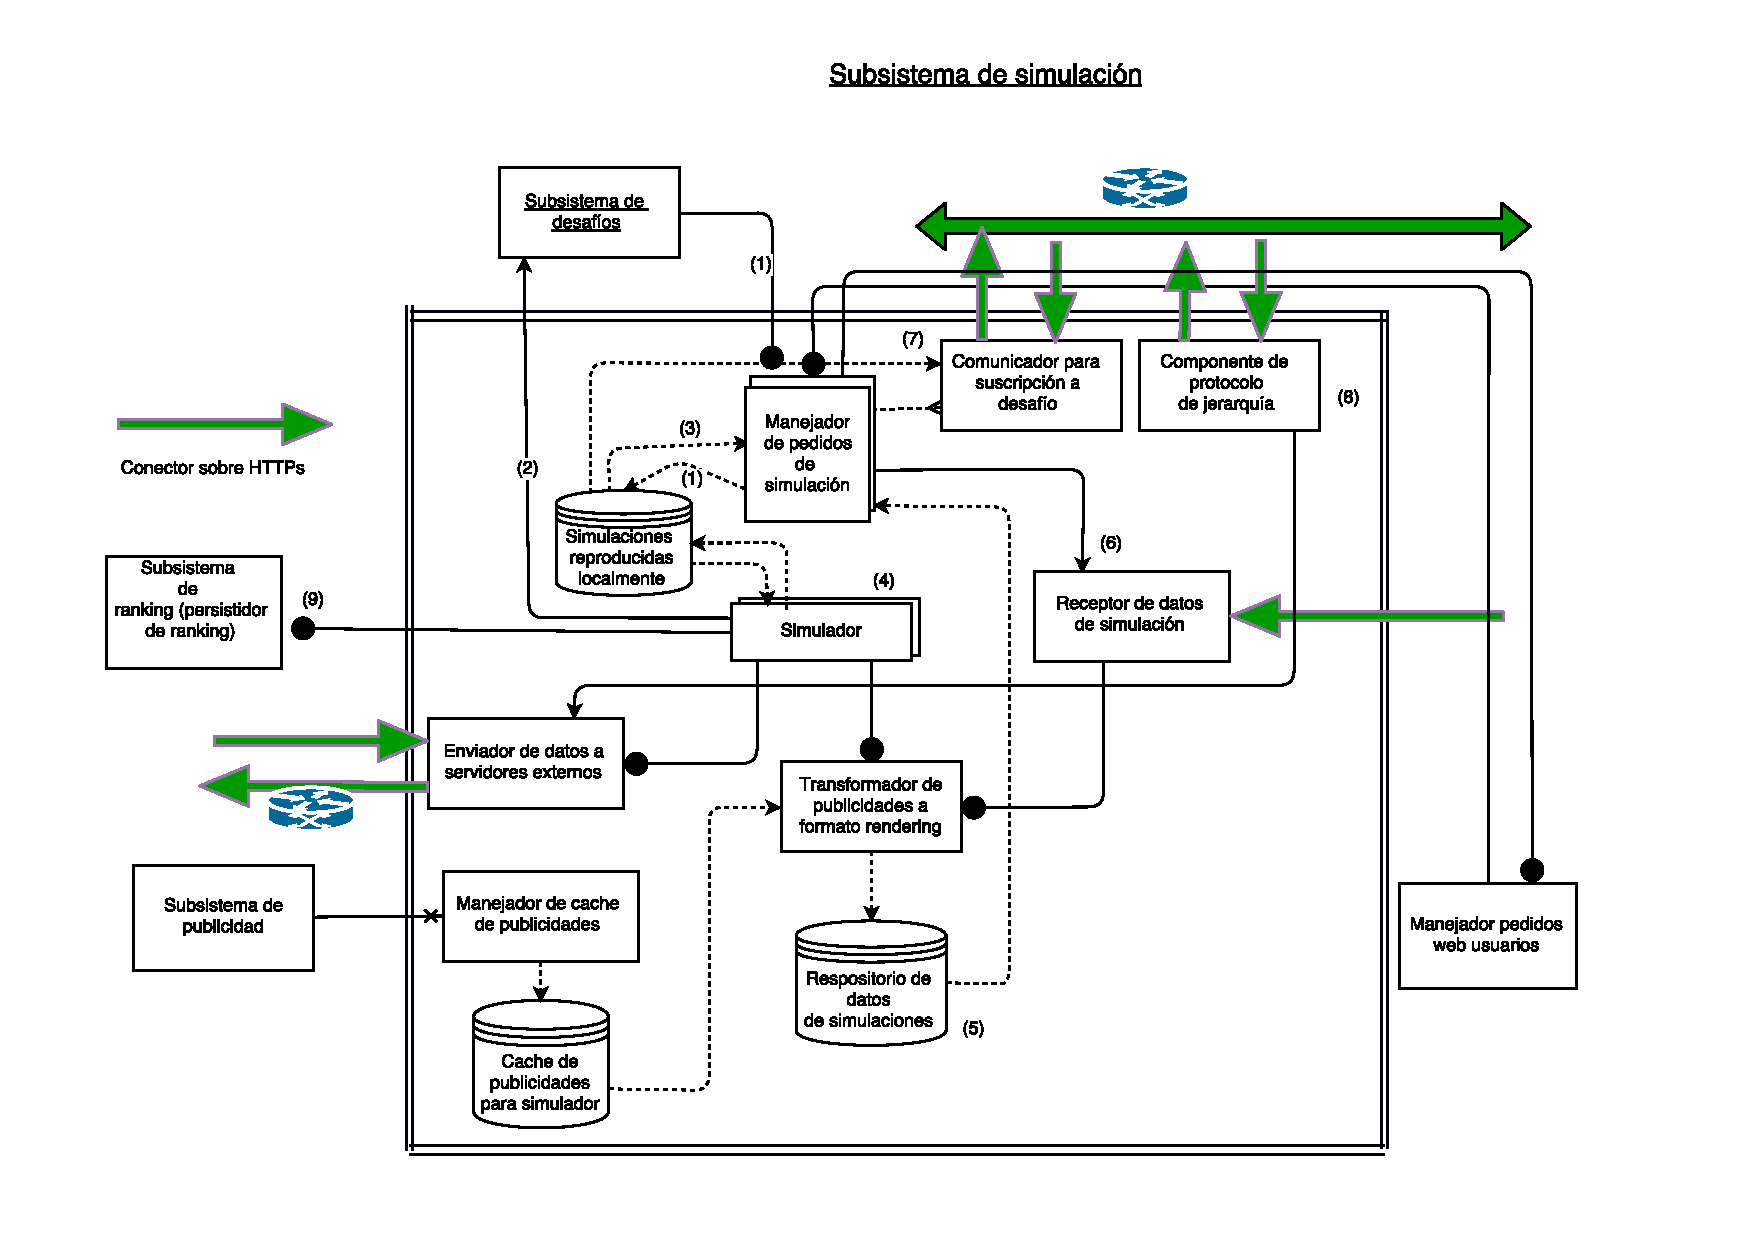
\includegraphics[width=1.1\textwidth, page=1, clip, trim=10 0 10 0]{imagenes/subs-simulacion.pdf}
  \caption{Subsistema de Simulacion.}
\end{figure}

\begin{figure}[H]
  \includegraphics[width=1.1\textwidth, page=2, clip, trim=25 0 10 0]{imagenes/subs-simulacion.pdf}
  \caption{Enviador Datos a servidores externos.}
\end{figure}

\begin{figure}[H]
  \includegraphics[width=1.1\textwidth, page=3, clip, trim=25 250 10 0]{imagenes/subs-simulacion.pdf}
  \caption{Receptor de datos de Simulacion.}
\end{figure}

\newpage

\subsection{Subsistema de Ligas de Fantasia}
\begin{figure}[H]
  \centering
  \includegraphics[width=\textwidth]{imagenes/fantasia.png}
  \caption{Subsistema de Ligas de Fantasia.}
\end{figure}

El procesador de comienzo de desafío almacena el desafío nuevo en el repositorio de desafíos activos, junto con todos los partidos a tener en cuenta.
Luego crea un procesador de comienzo de partido, que se encarga de revisar si el desafío indicado tiene algún partido que comenzar, y en caso que no sea así, programa un timer para
que le avise cuándo comienza el próximo partido. En este esquema, se crea un procesador de comienzo de partido para cada desafío nuevo que llega.
Cada vez que hay un partido, el procesador de comienzo de partido crea un procesador de minuto a minuto de partido. Este último, cada un minuto,
solicita al Subsistema de Estadisticas de Partidos las últimas actualizaciones. Con ellas evalúa las reglas de puntajes y actualiza los rankings (por ejemplo, una regla podría ser "Si mete gol, suma 3 puntos", y si una actualización
indica que Agüero metió un gol, entonces se envia al ranking A todos los participantes cuyo equipo tenga a Agüero suma 3 puntos).
Una vez actualizado los rankings, vuelve aprogramar el timer por un minuto. De esta manera habrá un procesador minuto a minuto por cada partido activo, que en cada minuto
actualizará los puntajes del ranking.\\

El procesador de comienzo de partido, luego de crear el de minuto a minuto, se programa
para el próximo partido. Si no hay más partidos, simplemente se destruye a sí mismo.\\

Cuando cada partido termina, el procesador de minuto a minuto se destruye a sí mismo, pero antes avisa del fin de partido al procesador de fin de partido, que verifica si
fue el último del desafio y en tal caso informa de la finalización del partido al subsistema de desafíos.

\newpage

\subsection{Subsistema de Ranking}
\begin{figure}[H]
  \centering
  \includegraphics[width=\textwidth]{imagenes/Subsistema-ranking.png}
  \caption{Subsistema de Rankings.}
\end{figure}

\newpage

\subsection{App Cliente}
\begin{figure}[H]
  \centering
  \includegraphics[width=\textwidth]{imagenes/Cliente.png}
  \caption{Applicacion del lado del Cliente.}
\end{figure}

\newpage

\subsection{Manejador pedidos Cliente}
\begin{figure}[H]
  \centering
  \includegraphics[width=\textwidth]{imagenes/Manejador-de-pedidos.png}
  \caption{Manejador de pedidos realizados por el cliente.}
\end{figure}

\newpage

\subsection{Subsistema de Usuarios}
\begin{figure}[H]
  \centering
  \includegraphics[width=\textwidth]{imagenes/manejo-usuarios.png}
  \caption{Subsistema de manejo de usuarios.}
\end{figure}

Cuando un usuario se registra, el manejador
ingresa la información en la base de datos.
Para interactuar con el sistema, el usuario
inicia una sesión.
Ante cada pedido, el sistema autoriza que el
usuario que generó el pedido tenga suficientes
permisos para hacerlo

\newpage

\subsection{Subsistema de Cobro y Pagos}
\begin{figure}[H]
  \centering
  \includegraphics[width=\textwidth]{imagenes/subs-cobro-y-pago.png}
  \caption{Subsistema de cobros y pagos.}
\end{figure}

Los datos de tarjetas y cuentas y el Tokenizador corren en una maquina distinta a todo el resto. Esto se hace para aislarla lo maximo posible y evitar cualquier vulnerabilidad que pueda llegar a tener el resto del sistema. Ademas estas maquinas deberan tener seguridad fisica, para evitar posibles robos y/o violaciones fisicas al sistema.

Funcionamiento:
\begin{enumerate}
\item {
  \begin{itemize}
  \item Caso medio de pago nuevo:
  Al manejador le llegan pedidos de pagos y/o cobros, autenticados y con informacion de un medio de pago nuevo. Entonces le pasamos esta informacion a el Tokenizador, que le genera un token, persiste en base de datos la informacion y el token correspondiente y le devuelve el token al Manejador de pedidos.
  \item Caso medio de pago existente:
  Al manejador le llegan pedidos de pagos o cobros, autenticados y con un id o refencia minima (elegida en por el Cliente) de que medio de pago se usara. Entonces con ese id o referencia, le pedimos al Tokenizador y obtenemos el token correspondiente.
  \end{itemize}
}

\item Luego con el token correspondiente, se lo brindamos al Realizador de pedidos, que entiende de tokens y con el se comunica con el medio de pago correspondiente y realiza la accion pertinente brindandole el token al medio de pago.

\item Luego con el resultado de la accion, la logeamos en el registro de movimiento y le devolvemos el resultado de la accion al Realizador y este al Manejador
\end{enumerate}

Ademas la información mas sensible (Numero de Tarjeta o Cuenta completa, codigo de seguridad de la tarjeta, etc) seran almacenada encriptada, mediante un algoritmo de clave asimetrica, donde la clave para desencriptar la tengan unicamente los dueños del sistema.

De esta forma, cumpliriamos con un estandar de seguridad llamado PCI, el cual es necesario para para poder realizar cobros y pagos con tarjetas de credito y cuentas bancarias. Este estandar sera todo el tiempo testeado para verificar que estemos siempre cumpliendo y en norma, ya que en caso de no estarlo estariamos abierto a posibles ataques y/o robos de datos.

\subsubsection{Biografia consultada}
\begin{itemize}
\item \href{https://www.pcisecuritystandards.org/documents/Tokenization_Guidelines_Info_Supplement.pdf}{Norma PCI.}\\
\item \href{https://www.quora.com/Do-companies-like-Amazon-etc-have-a-server-farm-to-store-creditcard-information-on-database}{Como cuidan sus datos compañias del estilo Amazon.}
\end{itemize}

\newpage

\subsection{Subsistema de Streaming}
\begin{figure}[H]
  \centering
  \includegraphics[width=\textwidth]{imagenes/subs-streaming.png}
  \caption{Subsistema de streaming de partidos reales.}
\end{figure}

La interacción entre el manejador de pedidos y el componente de streaming de partidos reales es análoga al de las simulaciones.
Los usuarios envían un pedido al manejador en donde solicitan ver el partido 'i'.
El manajador guarda una entrada en el repositorio en donde agrega una entrada que establece que el usuario 'u' está subscripto
al streaming del partido 'i'.

El manager de pedidos de streaming crea entonces una entrada en el 'repositorio de streams solicitados'. Este repositorio es 
consultado por el receptor de desafíos para saber a qué streamings generados por los proveedores de transmisiones suscribirse. 

Hay un conector custom por cada proveedor de servicios diferente

\newpage

\subsection{Subsistema de Publicidad}
\begin{figure}[H]
  \centering
  \includegraphics[width=\textwidth]{imagenes/Subsistema-de-publicidad.png}
  \caption{Subsistema de Publicidades.}
\end{figure}

La idea es que el manejador de pedidos stakeholders le indique al persisitidor de publicidades qué publicidad desea
guardar, indicándole en dónde deber mostrarse (transmisión de un partido, simulación o página principal del sitio) y en qué momento (hora).
Luego, el obtenedor de publicidades consulta periodicamente (cada 3 segundos) el repositorio solicitándole publicidades que deban mostrarse
en el momento en que consulta (+/- 3 segundos) y las envía a traves de un router a cada componente que hará uso del mismo (subsistema de
 simulación, subsistema de streaming y manejador de pedidos de usuario)

\newpage

\subsection{Subsistema de Estadisticas de Partidos}
\begin{figure}[H]
  \centering
  \includegraphics[width=\textwidth]{imagenes/Subsistema-de-estadistica-de-partido.png}
  \caption{Subsistema de Estadisticas de Partidos.}
\end{figure}

Los proveedores estadisticos que tenemos contratados publican actualizaciones periodicas de los partidos que se están disputando.
Como los datos publicados son propensos a errores decidimos utilizar un voter central que recibe las salidas de los múltiples procesadores y decide el
resultado correcto en función de los votos. Estos resultados son persisitidos en un repositorio el cual puede ser accedido mediante el obtenedor de
estadísticas de partidos.

\newpage

% \section{Arquitectura TP1}
% A continuación presentamos lo que seria un especie de Diagrama de Nivel 1 sobre la Arquitectura de la solución
del TP1.

\begin{figure}[H]
  \centering
  \includegraphics[width=\textwidth]{imagenes/TP1-Arquitectura.png}
  \caption{Arquitectura del TP1.}
\end{figure}

La idea basica es muy similar a la arquitectura propuesta en este trabajo practico, tenemos varios clientes
que nos realizan pedidos, en este caso serian consultas a los Rankings, consultas a las estadisticas de jugadores
y tecnicos o acciones respecto al sistema de desafios (creacion de cuentas, creacion de equipos, creacion de desafios,
manejo de fichas, etc). Todos estos pedidos son recibidos por el Manejador de Pedidos, el cual redirige cada pedido
al componente correspondiente.\\
Por otro lado en el componente Subsistema de Usuarios y Desafios, como ya dije estara toda la logica sobre el tema de
la creacion de equipos, desafios, etc. Este componente luego le brindara la informacion necesaria del desafio(Equipos, Jugadores, Tecnicos) al Subsistema de Simulacion para que este pueda simular el desafio. Luego una vez resuelta la simulacion, el subsistema de simulacion devuelve el log del partido para que el Subsitema de Usuarios y Desafios haga lo correspondiente, por un lado devolverle el resultado y el log al Manejador de pedidos para que le llegue al cliente, y por otro lado registrar el resultado, actualizar rankings, actualizar cap y pagar apuestas (en caso de ser necesario), etc.\\
El Subsistema de Simulacion para poder simular el desafio consume por un lado las estadisticas historicas de los jugadores y por otro lado las menciones en Twitter, para asi de esta forma tener los valores correspondientes a la hora de calcular los umbrales de exito.\\

Como podemos apreciar hay conceptos compartidos entre las dos Arquitecturas propuestas, pero la del Trabajo Practico 1 es mucho mas simple y chica, ya que la aplicacion en si era mas chica y menos compleja. No tenemos nada sobre ligas de fantasia, dinero real, tarjetas de credito, streaming de partidos reales, engines 2d y 3d para ver la simulacion, etc. Basicamente no teniamos ningun atributo de calidad por cumplir a raja tabla, por lo que es un Arquitectura pensada mucho mas en la funcionalidad que en otras cosas.

% \section{Comparaciones y Conclusiones}
% \subsection{UP vs Scrum}
Desde el punto de vista de la planificación, UP y Scrum se parecen en que ambas hacen un desgloce en tareas de cada uno de los módulos/user stories a realizar en la siguiente etapa/sprint. Sin embargo, UP realiza asignación de horas y tareas a cada recurso de antemano, mientras que en Scrum cada desarrollador elige la user storie que va a realizar cuando desea, siempre y cuando se llegue con los tiempos de entrega (finalización del sprint). En ambas metodologías se priorizan actividades: módulos o casos de uso en UP mediante el análisis de riesgos y user stories en Scrum mediante la estimación de esfuerzo y valor de negocio.

Desde el punto de vista de la ejecución de las actividades, UP las organiza en etapas mientras que Scrum en sprints. Estos difieren principalmente en que UP podría tener distinta duración de las iteraciones de distintas etapas (pero las iteraciones de una misma etapa duran lo mismo), mientras que en Scrum los sprints son todos de la misma duración. Además en UP se planifican los módulos que se tratarán en cada etapa desde el principio, mientras que en Scrum se elige el sprint backlog justo antes de cada sprint (de hecho podrían agregarse stories nuevas al backlog).

Scrum garantiza entregas en poco tiempo (idealmente al final de cada sprint), mientras que al final de las iteraciones de UP no necesariamente se pueden realizar entregas. Por otro lado, UP permite realizar una planificación a largo plazo de gran parte del proyecto, mientras que Scrum se va adaptando sobre la marcha y se actualiza el futuro del proyecto antes de cada sprint.


\subsection{Programming in the Small vs Programming in the Large}
Programming in the Small consiste en el modelado de sistemas pequeños, donde todos los detalles son conocidos de antemano y se puede modelar con un gran nivel de detalle. Los requerimientos no funcionales son poco exigentes: pocos usuarios, no hay grandes problemas de performance o disponibilidad; la modificabilidad se logra principalmente desde el diseño orientado a objetos; seguridad y usabilidad son los únicos atributos de calidad que podrían considerarse más en detalle.

Por otro lado, Programming in the Large consiste en el modelado de sistemas muy grandes, que no pueden diseñarse por completo usando clases y objetos, sino que se debe hacer un diseño de alto nivel, partir el problema en módulos (WBS) y atacar los módulos por separado y con una planificación detallada. Los atributos de calidad juegan un rol fundamental ya que la performance y disponibilidad del sistema suelen ser atributos muy importantes y difíciles de satisfacer. Además el dinero juega un papel importante ya que en la mayoría de las veces marcará la diferencia en la mejoría de la calidad del sistema.

PitL requiere una planificación mucho más detallada que PitS, ya que al tratarse de un proyecto de mayor duración teporal y de mayor consumo de recursos es importante que el uso de estos recursos se haga de manera eficiente. Los cambios de requerimientos en un proyecto grande van a generar un mayor impacto dependiendo de en qué fase del proyecto se realicen, es por esto que es fundamental la elicitación exhaustiva en las primeras etapas para evitar cambios de último momento que atrasen la finalización. En cambio las modificaciones en requerimientos de un proyecto pequeño se pueden tratar en todo momento dado que un impacto grande siempre estará limitado por el tamaño del proyecto que sigue siendo pequeño.

\subsection{Conclusiones}
En general para proyectos de PitS conviene utilizar metodologías ágiles como Scrum, ya que permiten generar entregables rápidamente. En un proyecto PitL las entregas a corto plazo pueden no ser factibles al principio porque quizás haya que construir muchos módulos antes de poder ver algún resultado interesante. Además Scrum permite el cambio de requerimientos antes de cada sprint, mientras que en UP se espera que los cambios de requerimientos sean sólo al principio del proyecto. Pero esto último no sirve para PitS dado que los cambios en requerimientos podrían surgir en cualquier momento, luego de que el cliente vea un entregable y cambie de opinión con respecto a cosas que había pedido previamente.

Por otro lado, los proyectos de PitL se acoplan mejor con UP ya que este provee un marco de planificación detallada muy necesario para proyectos grandes, que permite llevar el control global del proyecto. El esfuerzo y los recursos consumidos en la planificación son muy necesarios para PitL para evitar problemas futuros: el análisis y mitigación de riesgos es la clave para evitar problemas. En cambio Scrum prioriza actividades según valor de negocio, que en PitL podrían ser muchas y luego de varios meses de desarrollo podrían surgir problemas en módulos que no eran prioritarios para el negocio pero sí riesgosos para el funcionamiento correcto (por ejemplo, cuestiones de seguridad). Además en PitL no se esperan grandes cambios en los requerimientos (al menos no a nivel global, siempre podría haber pequeños cambios en los módulos), con lo cual Scrum sería demasiado flexible en este aspecto.

Por ende en general veremos Scrum aplicado a proyectos pequeños con requerimientos cambiantes y priorización según valor de negocio, y UP a proyectos grandes que requieren planificación a largo plazo y priorización según riesgos para evitar problemas.



% Ejemplo insertar imagen desde un pdf (mas facil cuando hay muchas paginas)

% \begin{figure}[H]
%   \includegraphics[width=1.1\textwidth, page=3, clip, trim=25 250 10 0]{imagenes/subs-simulacion.pdf}
%   \caption{Receptor de datos de Simulacion.}
% \end{figure}

% Ejemplo de insertar imagen png

% \begin{figure}[H]
%   \centering
%   \includegraphics[width=\textwidth]{imagenes/Subsistema-de-estadistica-de-partido.png}
%   \caption{Subsistema de Estadisticas de Partidos.}
% \end{figure}

\tableofcontents

\newpage
\section{Reentrega}
\subsection{Introducción}

En esta nueva solución, haremos foco en la distribución de los datos y el software.

Dado que se accederá al sistema potencialmente desde todas partes del mundo, no podemos tener un único servidor o conjunto de servidores que atiendan los pedidos porque necesitamos {\bf escalabilidad}. Entonces decidimos adoptar una arquitectura del estilo \emph{layered}, de tal manera que cada nivel tenga responsabilidades distintas y almacene datos distintos. Además estos niveles estarán asignados a servidores conectados con una topología lógica de árbol, donde las hojas corresponden a los clientes y la raíz a un nivel superior. Esto fuerza a que los pedidos suban y bajen en el árbol para llegar desde el punto A al punto B, evitando la saturación de un nodo muy solicitado (se evita que todos accedan al mismo tiempo a un nodo).

Concretamente, nuestro sistema tendrá 5 niveles:
\begin{enumerate}
	\item Internacional.
	\item Continental o regional.
	\item País.
	\item Estado/Provincia y Ciudad.
	\item Servidor web de clientes dentro de una Ciudad o pueblo.
\end{enumerate}

Los clientes realizarán pedidos únicamente a los servidores de nivel 5 (salvo la primera solicitud DNS, que la realizarán a root, ver sección \ref{seccionDNS}). Los servidores de nivel 5 manejan sesiones y comunicación web, pero no tienen datos. Entonces envían sus pedidos a los servidores de nivel 4, que almacenan datos de usuarios allí registrados y desafíos creados por esos usuarios (ver sección \ref{seccionAdmDatos}). En general los pedidos serán resueltos a nivel 4 (Provincia-Ciudad) o entre distintos nodos de nivel 4 pertenecientes al mismo país. Esto permite que el ``scope'' de los desafíos sea a nivel nacional, impidiendo que se pueda acceder desde un nodo interno de un país a un nodo interno de otro país.

Los nodos de nivel 3 almacenan desafíos creados a nivel nacional por los administradores y el ranking nacional. Los nodos de nivel 2 almacenan los desafíos creados a nivel Continental y el ranking continental. Y finalmente el de nivel 1 almacena los desafíos internacionales y el ranking internacional. Además cada nodo ejecuta los desafíos que hostea.

Además de la estructura de árbol, cada nodo en esta estructura está unívocamente identificado por un nombre llamado ``GeoPath''. Este nombre se representa como una tupla que indica el nombre geográfico de cada nivel para acceder un nodo, siguiendo este esquema:
\begin{center}
	$<$Continente, País, Estado/Provincia, Ciudad$>$
\end{center}

Por ejemplo, el único nodo de nivel 1 (la raíz del árbol) tiene GeoPath ``$<$ $>$''. El continente sudamericano (nivel 2) tiene GeoPath ``$<$Sudamérica$>$''. Argentina (nivel 3) tiene GeoPath ``$<$Sudamérica, Argentina$>$''. Y la ciudad de buenos aires tiene GeoPath ``$<$Sudamérica, Argentina, Bs.As., CABA$>$'' (nivel 4). Los nodos de nivel 5 no necesitan GeoPath dado que no almacenan datos y no es necesario referenciar específicamente uno de ellos (son todos iguales los nodos de nivel 5 que corresponden a cada nodo de nivel 4 ya que no almacenan datos).

Internamente en cada nodo hay cero o más réplicas, tanto de software como de datos. Las réplicas de datos son sincronizadas utilizando redundancia pasiva por el administrador de datos (ver sección \ref{seccionAdmDatos}). Las réplicas de software se acceden utilizando un esquema de favoritismo, donde una de las réplicas es la favorita de ciertos nodos, pero si esa se cae, se utiliza otra aleatoriamente.

Todos los números o decisiones tomadas aleatoriamente se basan en una distribución uniforme de la probabilidad, que a largo plazo permite distribuír la carga de forma equitativa.


A continuación presentaremos distintos diagramas correspondientes a la vista de componentes y conectores de la arquitectura planteada junto con la explicación de cada uno y el deployment de algunos componentes.
\subsection{Referencias}

Se presenta un listado de los conectores y notación especial utilizada en los diagramas, a modo de referencia. Además se provee el zoom sobre algunos conectores especiales.

\begin{figure}[H]
   \centering
   \includegraphics[width=\textwidth]{reentrega/imagenes/referencias1.png}
   \caption{Referencias de diagramas (Parte 1).}
\end{figure}

\newpage

\begin{figure}[H]
   \centering
   \includegraphics[width=\textwidth]{reentrega/imagenes/referencias2.png}
   \caption{Referencias de diagramas (Parte 2).}
\end{figure}

\subsubsection{Client-Server Seguro (SSL)}

%\begin{figure}[H]
%   \centering
%   \includegraphics[width=\textwidth]{reentrega/imagenes/conector_ssl.png}
%   \caption{Zoom de conector Client-Server Seguro (SSL).}
%\end{figure}

La comunicación segura via SSL funciona de la siguiente manera. Supongamos que un cliente desea comenzar una comunicación segura con un servidor.

En primer lugar, le solicita al servidor sus certificados SSL, para verificar la autoridad. Solicita tanto la clave pública como los certificados y los compara con los que tiene almacenados localmente.

En el siguiente paso, el servidor le solicita al cliente que genere un número random. El cliente genera el número, lo encripta utilizando la clave pública para que sea el servidor el único que pueda leerlo y se lo envía.

El servidor obtiene este número, lo desencripta utilizando su clave privada, y posteriormente utiliza el número aleatorio para generar una clave simétrica. La clave es encriptada mediante un algoritmo conocido por el cliente utilizando el número aleatorio, y luego utilizando la clave privada. El cliente utiliza la clave pública para resolver la primera enriptación, y luego el desencriptador con el mismo número aleatorio que le ha enviado al servidor. En este momento, ambas partes tienen la clave simétrica que utilizarán posteriormente para encriptar y desencriptar los pedidos y las respuestas.

Ambos almacenan la clave simétrica en repositorios para su posterior uso. La clave simétrico expira cada cierto tiempo, por lo que el protocolo debe volver a ejecutarse.


\subsubsection{Client-Server Seguro con destinatario favorito}

%gráfico Referencias (página fila 1 columna 2)

El componente Enviador/Receptor intenta enviar el mensaje
al destinatario favorito (Servidor) mediante SSL y setea un timer.
Si el timer avisa, es decir si se produce un timeout, el componente
cierra la sesión SSL creada previamente y busca al azar entre los
demás destinatarios posibles, y repite el proceso. El destinatario
favorito se marca como ``inaccesible'' y se setea un timer en 10
minutos que avisará al componente ``Habilitador de destinatario
favorito'' que vuelva a habilitar el destinario favorito para
futuro uso.

La idea es que si el destinatario favorito vuelve a ser accesible se
vuelva a utilizar, pero se le da un tiempo antes de reintentar para
no saturarlo y poder seguir operando sin que se produzca timeout
en todos los pedidos (a causa de que el favorito está caido).

\subsubsection{Client-Server Seguro con caché en el cliente}

%gráfico Referencias (página fila 1 columna 4)

El ``Resovedor de request HTTP'' primero busca el recurso en la caché:
\begin{itemize}
	\item Si no lo encuentra, busca el request entre los que fueron enviados pero aún no respondieron:
	\begin{itemize}
		\item Si no lo encuentra, de manera atómica escribe el request en ese repositorio para indicar a futuros
        pedidos que ese request será cacheado a la brevedad. Luego envía el request al ``Enviador/Receptor de
        request/response HTTP'', el cual lo envía al servidor. Cuando recibe la respuesta, la escribe en la caché
        y luego marca el request con el flag de ``Cacheado'' en el repositorio de requests HTTP enviados. Finalmente
        devuelve el response al ``Resolvedor de request HTTP'', que se lo retorna al cliente.
        
        \item Si lo encuentra, se suscribe al blackboard de Requests enviados que aún no respondieron.
        Cuando el flag de ese request pasa a estar en ``Cacheado'', se dispara el evento
        a todos los suscriptos para que sepan que ya está cacheado el pedido. Luego el ``Resolvedor de
        request HTTP'' busca el pedido en la caché.
	\end{itemize}
	
	\item  Si lo encuentra en la caché, simplemente lo retorna.
\end{itemize}

En paralelo, hay un proceso ``Purgador de caché'' que cada X tiempo configurable borra las entradas
de caché que en ese tiempo no hayan sido usadas o que tengan TTL=0.


\subsubsection{Client-Server Seguro con destinatario favorito y caché en el cliente}

%gráfico Referencias (página fila 1 columna 3)

El ``Resovedor de request HTTP'' primero busca el recurso en la caché:
\begin{itemize}
	\item Si no lo encuentra, busca el request entre los que fueron enviados pero aún no respondieron:
	\begin{itemize}
		\item Si no lo encuentra, de manera atómica escribe el request en ese repositorio para indicar a futuros
        pedidos que ese request será cacheado a la brevedad. Luego envía el request al ``Enviador/Receptor de
        request/response HTTP'', el cual lo envía al servidor. Cuando recibe la respuesta, la escribe en la caché
        y luego marca el request con el flag de ``Cacheado'' en el repositorio de requests HTTP enviados. Finalmente
        devuelve el response al ``Resolvedor de request HTTP'', que se lo retorna al cliente.
        
        \item Si lo encuentra, se suscribe al blackboard de Requests enviados que aún no respondieron.
        Cuando el flag de ese request pasa a estar en ``Cacheado'', se dispara el evento
        a todos los suscriptos para que sepan que ya está cacheado el pedido. Luego el ``Resolvedor de
        request HTTP'' busca el pedido en la caché.
	\end{itemize}
	
	\item  Si lo encuentra en la caché, simplemente lo retorna.
\end{itemize}

En paralelo, hay un proceso ``Purgador de caché'' que cada X tiempo configurable borra las entradas
de caché que en ese tiempo no hayan sido usadas o que tengan TTL=0.
\subsection{Esquema general de interacción entre niveles y administrador de pedidos de nivel i}

\begin{figure}[H]
   \centering
   \makebox[\textwidth][c]{\includegraphics[width=1.2\textwidth]{reentrega/imagenes/todos-los-niveles-macro.png}}
   \caption{Vista de todos los niveles en simultaneo.}
\end{figure}

\begin{figure}[H]
   \centering
   \makebox[\textwidth][c]{\includegraphics[width=1.2\textwidth]{reentrega/imagenes/todos-los-niveles-administrador-pedidos.png}}
\end{figure}

Un administrador de pedidos es el encargado de responder consultas provenientes de niveles inferiores respecto a consultas de desafíos y ranking general. Cuando el administrador de datos tiene la información suficiente para responder al pedido, el
mismo se resuelve en el momento. Por ejemplo, supongamos que Juan es un usuario de Córdoba y crea un desafío con id = 35.
Si Pedro también es cordobés, al preguntar por el desafío de id=35 el administrador de pedidos de nivel 4 (provincia=Córdoba) va a contar con la información necesaria para responder.
Distinto es el caso en el que Pedro consulta por un desafío que fue creado por un administrador a nivel nacional. En este caso, los datos van a ser manejados por el administrador de pedidos de nivel 3 (país=Argentina). En este caso, se forwardea el
pedido para que sea resuelto por este último.
El mismo mecanismo se produce de manera recursiva hasta llegar al nivel global.

Los administradores pueden crear en desafíos en cada nivel, cuyos datos serán almacenados en el administrador de pedidos
correspondientes. De esta manera se guardan datos de desafíos de los mejores a nivel mundial en el adm. nivel 1 y a nivel continental en el nivel 2. A nivel país, los administradores pueden crear desafíos que excedan a las provincias. Como por ejemplo, un gran DT en donde a priori se sabe que va a participar todo el país. Si esto fuera almacenado a nivel 4, todo el país debería acceder a ese mismo nodo de nivel 4.

El componente ``Procesador de Solicitudes HTTP iniciales, geolocalización de IPs y monitoreo de servidores de nivel 5'' sólo se utiliza a nivel 1 para redirigir usuarios que acceden por primera vez por DNS al servidor de nivel 5 correspondiente a su zona.

Una diferencia entre el nivel 4 y los demás es que existe comunicación horizontal entre los administradores del mismo nivel. Por ejemplo, si Juan creo un desfío en Córdoba y Rodrigo de Tucumán quiere ver el listado de desafíos Cordobeses para poder inscribirse en alguno, los administradores de pedidos cuentan con un bus de comunicación sin necesidad de utilizar
al padre (de nivel 3: país=Argentina) como intermediario. Esto se hace para no sobrecargar de pedidos al componente
que responde pedidos a nivel país. Por el contrario, como ya se mencionó anteriormente, si Rodrigo quiere ver el resultado de la fecha de Gran DT, el componente administrador de nivel 4 deberá forwardear el pedido al de nivel 3.

Otra diferencia entre el nivel 4 y los demás es que en el componente administrador de usuarios dejan de tener sentido algunos componentes como por ejemplo el autenticador o el registrador de usuario ya que los usuarios nunca se van a registrar en los niveles superiores.

A nivel país y continental no hay comunicación a nivel horizontal entre cualquier par de nodos, sólo puede haber comunicación entre hermanos del mismo padre. Por ejemplo, no se puede comunicar el nodo de Argentina con el de España, pero sí el de Argentina con el de Uruguay ya que ambos pertenecen al nodo padre ``Sudamérica''. Los pedidos de regiones superiores siempre se propagan hacia arriba. Rodrigo, de Tucumán puede consultar: desafíos nacionales de Argentina, desafíos sudamericanos y desafíos mundiales. El pedido es forwardeado hasta el nivel que corresponde y luego desciende hasta el
manejador de nivel 5 que generó el pedido. Para evitar sobrecargar a los niveles superiores (que potencialmente son los que pueden recibir mayor cantidad de pedidos), las respuestas se van cacheando en los niveles intermedios. Por ejemplo,
si todos los usuarios de Sudamérica están preguntado por los resultados del desafío mundial de Básket los resultados
se cachean en los administradores de nivel 4 (provincias), de nivel 3(país) y de nivel 2 (continente=Sudamérica), durante un tiempo máximo configurable.


El administrador de pedidos de nivel i también es el encargado de propagar los datos de los renderizadores para simulación, el streaming de partidos reales y los datos de las ligas reales para que los desafíos de tipo liga de fantasía puedan resolverse
en los demás administradores.
Las 3 tipos utilizan buses de publisher/suscriber.
Tanto la lógica del streaming de partidos reales como los datos de las ligas realesutilizados para resolver los desafíos es la siguiente: Como un usuario puede elegir equipos y armar desafíos de ligas de cualquier parte del mundo, independientemente de dónde viva, entonces cada nivel debe poder su suscribirse tanto al nivel superior como al inferior. Los niveles superiores se utilizan como intermediarios para alcanzar nodos en otras ramas.

Ejemplo: Rodrigo de Tucumán creo un desfafío de basquet utilizando la NBA como liga. Por lo tanto, le gustaría por un
lado poder ver los partidos de la NBA para ir siguiendo sus resultados. Al mismo tiempo, el componente administrador
de Tucumán deberá comenzar a recibir los datos de los partidos de la NBA para calcular los resultados. Estos datos
son provistos por las empresas proveedoras al componente administrador de nivel 3, país=EE.UU.
Entonces el flujo de la suscripción funciona de la siguiente forma. El \textbf{bus del administrador de flujo de streaming} del componente administrador de nivel 4 (provincia = Tucumán)
desea subscribirse al streaming del partido de Spurs vs LA Lakers. Como actualmente no está streameando dicho partido,
se comunica y suscribe all bus de administrador del flujo de streaming de nivel 3 (país=Argentina). Como este tampoco está streameando, se comunica y suscribe al bus del nivel 2 (continente=Sudamérica). Como este tampoco está streameando, se
comunica con el  nivel 1 (Global). Este utiliza el identificador del partido (que contiene el GeoPath) e identifica que el evento es de América del Norte, por lo tanto
se suscribe a dicho partido en el bus de América del Norte. El servidor de América del Norte identifica que el partido se
está jugando en EEUU, por lo que se suscribe al mismo en el bus de dicho país. Finalmente, al llegar el pedido el componente
administrador de EEUU se suscribe al proveedor de transmisiones de la NBA y comienza a recibir la transmisión del partido.
En el proceso se armó la cadena de suscripciones necesaria para recibir los datos. Si algún otro usuario de Argentina o Sudamérica quisiera comenzar a recibir la transmisión también el proceso no tiene necesidad de repetirse.
La lógica de los suscribers y los publishers es parte del conector. De esta manera podemos reutilizar la lógica en cada
nivel, sin necesidad de repetir los componentes.

Finalmente, los datos de la simulación funcionan de forma vertical únicamente, tal como los desafíos. Usuarios de distintos países
o continentes no tienen la necesidad de ver simulaciones compartidas. Por lo tanto, cada componente administrador
se suscribe a lo sumo al nivel i-1 (en caso de que la simulación no esté siendo generada por él mismo), y los paquetes
se propagan de jerarquía mayor a menor dentro de una misma rama.

\newpage

\subsection{Administración de datos} \label{seccionAdmDatos}

% gráficos de ADM de datos (las tres páginas seguidas, y luego la explicación).
\begin{figure}[H]
   \centering
   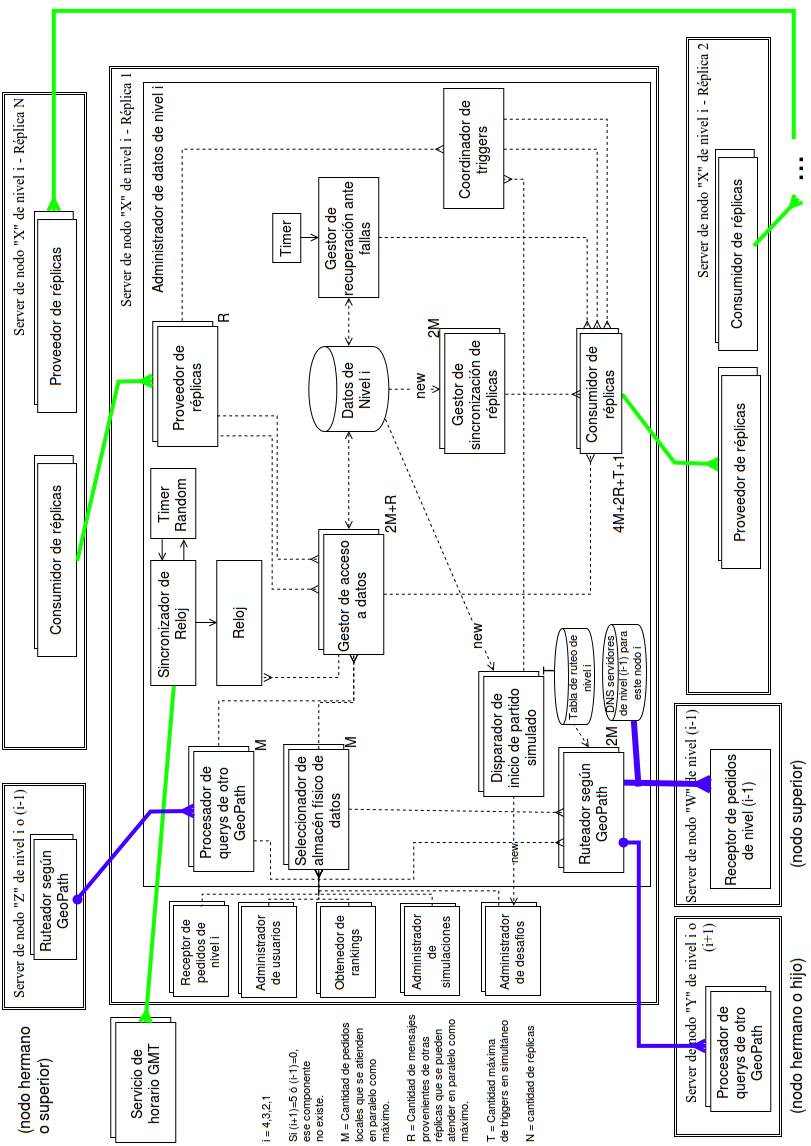
\includegraphics[height=0.93\textheight]{reentrega/imagenes/admDatos.png}
   \caption{Componente administrador de datos de nivel i.}
\end{figure}

\begin{figure}[H]
   \centering
   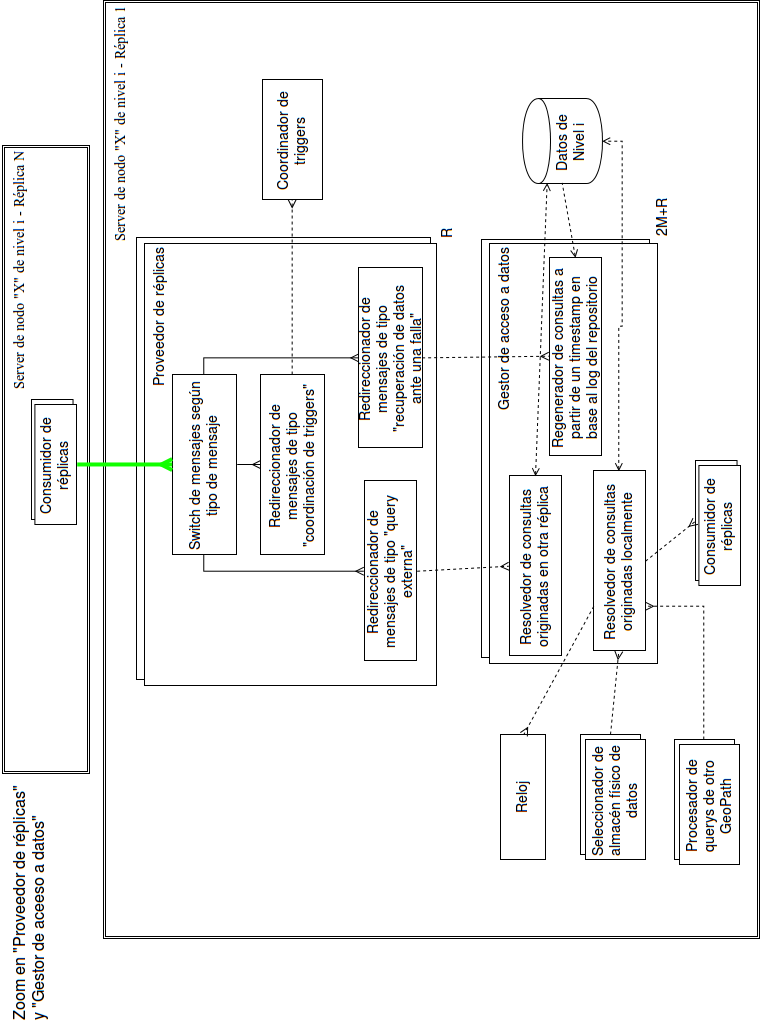
\includegraphics[height=0.93\textheight]{reentrega/imagenes/admDatos-zoom1.png}
   \caption{Zoom en ``Proveedor de réplicas'' y ``Gestor de acceso a datos''.}
\end{figure}

\begin{figure}[H]
   \centering
   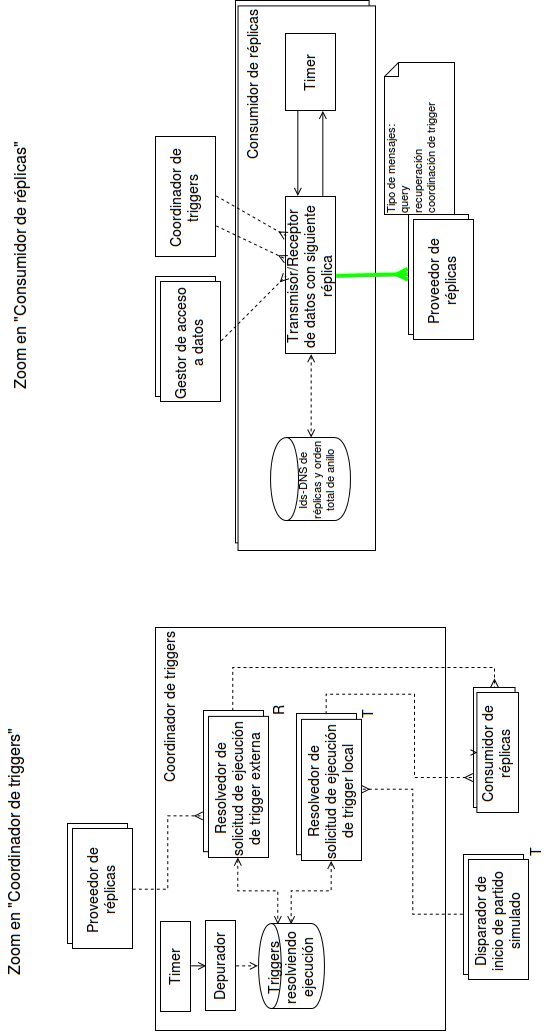
\includegraphics[height=0.93\textheight]{reentrega/imagenes/admDatos-zoom2.png}
   \caption{Zoom en ``Proveedor de réplicas'' y ``Coordinador de triggers''.}
\end{figure}

En cada nodo de nivel i (Ej: CABA en nivel 4) hay uno o más servidores. Cada uno tiene un servidor HTTP  y un Data Server con los datos de ese nodo. Todos los servidores en un mismo nodo son réplicas tanto de software como de datos. Por ejemplo, para el GeoPath $<$Sudamérica, Argentina, Bs.As., CABA$>$ tenemos 10 servidores de nivel 4, donde cada uno tiene el mismo software y los mismos datos.

Los relojes de todos los servidores de nivel i están sincronizados.
Dentro del componente ``Administrador de Datos'' hay un ``Sincronizador de Reloj'' que se ejecuta cada cierta cantidad de minutos entre 1 y 5, definida aleatoriamente cada vez. Este componente accede a un servicio online que provee la hora GMT. Los minutos se eligen aleatoriamente para evitar que todos los servidores accedan al mismo tiempo al servicio web y lo saturen. El proveedor del servicio nos confirmó que usando esta  estrategia el servicio respondería siempre. Además nos aseguró que tiene una réplica de su servicio hosteada en cada país, para reducir el tiempo de respuesta. De esta manera, todos los servidores de nivel i se encuentran sincronizados al horario GMT.

Cada registro en los repositorios de datos tiene asociado un timestamp correspondiente a la última actualización.

\subsubsection{Replicación de datos y manejo de fallas}

Cada servidor escribe y lee los datos de su réplica local, salvo que ésta no responda. Supongamos primero que la réplica local funciona correctamente. Luego de realizar una escritura, el “Seleccionador de almacén físico de datos” envía la query al “Gestor de Acceso a Datos” por determinado puerto, que le indica al gestor que la query se originó localmente. Luego le asigna un timestamp (TS) a la query y la ejecuta en el repositorio local. Si la query produjo un cambio en los datos, se dispara automáticamente el proceso “Gestor de sincronización de réplicas” (con un trigger) al que se le asigna como input la metadata de los cambios producidos en los datos locales. Este genera una query para actualizar y sincronizar las demás réplicas, la cual incluye el timestamp generado previamente (TS).

La estructura de réplicas tiene forma de anillo, donde cada par de réplicas se comunica utilizando “Consumidor de réplicas” y “Proveedor de réplicas”, mediante un conector seguro (SSL). Entonces el “Gestor de sincronización de réplicas” envía la query con el TS al “Consumidor de réplicas” y este a su vez envía la query al “Proveedor de réplicas” del siguiente servidor en el anillo.

El “Proveedor de réplicas” luego envía la query al “Gestor de acceso a datos” por un puerto especial, que le indica que la query es externa, entonces antes de impactarla, verifica los datos que serán alterados y compara el TS con el TS de cada registro. De esta manera detecta si localmente hay una actualización posterior a la que llegó de afuera (o si ya tiene la misma), y en tal caso la descarta y no la impacta. Este mecanismo no sólo prioriza la escritura más reciente para evitar condiciones de carrera sino que además permite cortar el ciclo de actualizaciones (cuando llega nuevamente a la réplica que originó la actualización, el TS de la query y del registro será el mismo y no se impactará).

Cabe aclarar que si una query externa fue descartada porque la copia local contenía un dato más nuevo, este dato ya fue enviado hacia las siguientes réplicas del anillo, por ende no tiene sentido propagar la query externa que quedó vieja.

Ahora veremos el caso en el que la réplica local de datos falla y debemos utilizar una réplica externa. En tal caso, el “Gestor de acceso a datos” detectará con un timeout que hubo un problema en la copia local y encenderá internamente un flag indicando que la copia local no se puede usar. Además seteará un timer para que en 10 minutos se apague el flag y se pueda reintentar con la copia local.

Dado que la query se generó en este servidor, aunque no haya podido impactarse, le agrega un timestamp y luego la envía al “Consumidor de réplicas”, que la transmite y la impacta usando el “Proveedor de réplicas” de la misma manera que antes.

Si llega una query al “Proveedor de réplicas” mientras la réplica local está inutilizable, el componente la envia al “Gestor de acceso a datos”, el cual la redirige al “Consumidor de réplicas” sin siquiera intentar utilizar el repositorio local (hasta que se apague automáticamente el flag).

Todo el mecanismo descripto se basa en la estrategia transaccional utilizada por Cassandra. Localmente en cada repositorio utiliza transacciones ACID (que garantizan principalmente la atomicidad y durabilidad de las escrituras) y a nivel global se garantiza consistencia eventual (asumimos que los datos terminan de propagarse por el anillo en a lo sumo 30 segundos). Esto permite tener las réplicas eventualmente consistentes, garantizando alta disponibilidad (si una réplica falla) y performance (no es necesario escribir en todas las réplicas y esperar ACKs por cada transacción). La única desventaja es que si se acceden a dos réplicas distintas en un intervalo muy corto de tiempo podrían verse datos distintos, pero como los servidores de nivel 5 tienen preferencia por uno de nivel 4 y siempre usan el mismo (salvo fallas), en general un mismo usuario accederá siempre al mismo servidor de nivel 4 y verá los mismos datos. Si un usuario crea un desafío, quizás sus amigos tengan que refrescar el sitio varias veces para ver el nuevo desafío en la lista.

\subsubsection{Triggers programados por reloj}

Los partidos de los desafíos registrados en un nodo de nivel i son ejecutados en el mismo nodo (simulados o liga de fantasía). Pero cada partido podría ejecutarse en cualquiera de las réplicas dentro del nodo. Físicamente, el trigger que dispara el inicio de un partido a determinada hora se registra en todas las réplicas. Dado que comparten el reloj, deberían disparar el trigger todas al mismo tiempo aproximadamente. Una vez que el trigger es disparado, lo recibe el “Disparador de inicio de partido simulado”, que antes de enviarlo al “Administrador de Desafíos”, le envía una consulta a un “Coordinador de Triggers”, indicando todos los metadatos necesarios para identificar el trigger disparado por el repositorio.

Dentro del “Coordinador de Triggers”, la solicitud es procesada por “Resolvedor de solicitud de ejecución de trigger local” que almacena en un repositorio interno los metadatos del trigger (IdTrigger) y luego genera un número aleatorio entre 0 y 1 (Rnd). Si el IdTrigger ya se encontraba en el repositorio, debería haber un flag indicando que no será ejecutado localmente, y el proceso termina (ver más adelante por qué puede suceder esto). Finalmente, envía un mensaje al “Coordinador de Triggers” que está siguiente en el anillo (mediante el “Consumidor de réplicas”), indicando los siguientes datos:

\begin{itemize}
	\item IdTrigger
	\item Id de la réplica donde se originó el trigger (ej: 1)
	\item Número aleatorio más grande encontrado para la ejecución de este trigger (Rnd)
	\item Id de la réplica que tiene el número aleatorio más grande
\end{itemize}

Este paquete debe dar toda la vuelta en el anillo. A medida que vaya pasando por cada “Coordinador de Triggers” del anillo, estos observarán el número aleatorio que generaron localmente y si es más grande, cambiarán los últimos dos campos (en breve explicaremos cómo). Luego de dar toda la vuelta, el paquete llega al “Coordinador de triggers” de la réplica original, que detectará que es la original por el segundo campo, y luego observa el último campo, que indica quién ejecutará el trigger. De esta manera, la réplica que haya obtenido el número aleatorio más alto ejecutará el trigger.

Dentro del “Coordinador de Triggers” se encuentra el “Resolvedor de solicitud de ejecución de trigger externa”, que recibirá paquetes como el descripto previamente, proveniente de la réplica anterior en el anillo. Este componente tomará cada paquete e inspeccionará primero el segundo campo:

\begin{enumerate}
	\item Si el paquete se originó en la réplica actual, quiere decir que ya dio toda la vuelta al anillo y el cuarto campo indica qué réplica debe ejecutar el trigger. Entonces en el repositorio de “Triggers resolviendo ejecución” se marca con un flag si debe ejecutarse localmente o no. Luego el “Resolvedor de solicitud de ejecución de trigger local” que había tomado la solicitud inicial observará el cambio en el repositorio y responderá a quién lo solicitó.

	\item Si el paquete se originó en otra réplica, compara el número aleatorio con el número aleatorio local (que lo lee de “Triggers resolviendo ejecución”). Si es más grande el local, se actualiza el paquete y se envía al siguiente en el anillo. Si casualmente el número aleatorio es igual (un caso muy poco probable), se utiliza el id de réplica para desempatar (gana la más grande).

\begin{enumerate}
		\item Si por alguna razón el IdTrigger no se encuentra en “Triggers resolviendo ejecución”, se agrega el IdTrigger al repositorio y se marca con el flag de que no será ejecutado localmente, y el paquete se pasa al siguiente en el anillo tal cual se recibió. De esta manera si el trigger es disparado más tarde localmente, directamente se desestima ya que fue ejecutado en otra réplica.
\end{enumerate}
\end{enumerate}


De esta manera hay una única réplica que ejecuta la simulación de un partido, ya que sólo un “Administrador de datos” enviará el disparador hacia el “Administrador de desafíos”. La ejecución de un trigger se podrá demorar a lo sumo 30 segundos (el tiempo máximo en dar una vuelta al anillo).

Cada 24hs se ejecuta un “Depurador” que borra las entradas de “Triggers resolviendo ejecución” que ya están resueltas (flag de ejecución o no ejecución encendido) hace más de 24hs.


\subsubsection{Recuperación ante fallas}

Si un servidor del anillo falla en su totalidad (o falla la comunicación), el componente “Consumidor de réplicas” internamente setea un timer cada vez que envía un mensaje. Si el timer genera un aviso (timeout), componente “Transmisor/Receptor de datos con siguiente réplica” inspecciona su repositorio interno donde tiene la estructura del anillo y busca el siguiente integrante del anillo. Entonces se comunica directamente con el siguiente en el anillo.

Cuando un servidor vuelve a levantarse (o cuando el repositorio vuelve a funcionar), hay un proceso que está continuamente monitoreando el repositorio y descubre este evento (“Gestor de recuperación ante fallas”). Este proceso se encarga de verificar los logs del repositorio para ver el timestamp de la última transacción y envía un pedido de recuperación con ese timestamp al “Consumidor de réplicas”. Este mensaje llega a través del “Proveedor de réplicas” al “Gestor de acceso a datos” (por un canal especial). Luego el “Gestor de acceso a datos” busca todas las actualizaciones que hubo en su repositorio local desde el timestamp indicado hasta el momento y las retorna por el mismo canal. Estas actualizaciones llegan nuevamente al “Gestor de recuperación ante fallas”, que persiste los datos verificando los timestamps (por si ya hay datos nuevos en el repositorio recuperado). 


\subsubsection{Acceso a nodos de distinto GeoPath}

Esto lo detecta el “Seleccionador de almacén físico de datos”, que en caso de no corresponder el GeoPath al nodo actual, lo envía al “Ruteador según GeoPath”. Este componente utiliza una “Tabla de ruteo de nivel i”. Esta tabla permite rutear la solicitud a:

\begin{itemize}
	\item Un nodo hijo de este GeoPath, de nivel i+1 (Ej: de $<$Sudamérica,Argentina$>$ ir a $<$Sudamérica, Argentina, Bs.As., CABA$>$, pero no a $<$Europa, España, Barcelona, Barcelona$>$). Si i=4 esto no es posible ya que en nivel 5 no hay datos.
	\item Un nodo hermano de este GeoPath, de nivel i (Ej: de $<$Sudamérica,Argentina$>$ ir a $<$Sudamérica, Chile$>$, pero no se puede ir a $<$Europa, España$>$).
	\item El nodo superior de este GeoPath, de nivel i-1 (Ej: de $<$Sudamérica,Argentina$>$ ir a $<$Sudamérica$>$, pero no a $<$Europa$>$). Si i=1, no es posible esta navegación porque no hay nodo superior.
\end{itemize}

Este esquema permite que desde cualquier nodo se pueda escribir en cualquier otro usando el GeoPath correcto, pero la navegación se realiza a través del árbol sin saltear niveles. Esto reduce la cantidad de pedidos que puedan subir al nivel 1 desde muchos de nivel 4 y a la vez impide que haya muchos servidores de distintos niveles y regiones que escriban datos en un mismo nodo de nivel 4 (que contiene datos de usuarios y es posible que muchas veces sea necesario hacerlo).

Las tablas de ruteo tienen para cada GeoPath varios nombres de dominio de las distintas réplicas del nodo que cubre ese GeoPath.

Por ejemplo:
\begin{itemize}
	\item Tabla de ruteo de nivel 1 podría contener: (observar que no contiene entrada de nivel 1 porque no hay otro nodo de nivel 1, sólo hay réplicas).
	
	\begin{center}
	\begin{tabular}{| c | c |}
	\hline
	GeoPath & DNS \\
	\hline
	$<$Sudamérica$>$ & sudamerica.n2.s1.currygame.com, sudamerica.n2.s2.currygame.com\\
	\hline
	$<$África$>$ & africa.n2.s1.currygame.com\\
	\hline
	\end{tabular}
	\end{center}
	
	\item Tabla de ruteo de nivel 2 de Sudamérica podría contener:

	\begin{center}
	\begin{tabular}{| c | c |}
	\hline
	GeoPath & DNS \\
	\hline
	$<$Sudamérica,Argentina$>$ &  ar.n3.s1.currygame.com\\
	\hline
	$<$África$>$ & africa.n2.s1.currygame.com\\
	\hline
    $<$ $>$ &  n1.s1.currygame.com\\
	\hline
	\end{tabular}
	\end{center}
	
	\item Tabla de ruteo de nivel 3 de Argentina podría contener:
	\begin{center}
	\begin{tabular}{| c | c |}
	\hline
	GeoPath & DNS \\
	\hline
	$<$Sudamérica, Argentina, Bs.As., CABA$>$ & caba.ar.n4.s1.currygame.com\\
	\hline
	$<$Sudamérica,Argentina$>$ &  ar.n3.s1.currygame.com\\
	\hline
	$<$Sudamérica$>$ &  sudamerica.n2.s1.currygame.com\\
	\hline
	\end{tabular}
	\end{center}
	
	\item Tabla de ruteo de nivel 4 de CABA podría contener:
	\begin{center}
	\begin{tabular}{| c | c |}
	\hline
	GeoPath & DNS \\
	\hline
	$<$Sudamérica,Argentina$>$ &  ar.n3.s1.currygame.com\\
	\hline
	$<$Sudamérica, Argentina, Bs.As., Lanús$>$ & lanus.ar.n4.s1.currygame.com\\
	\hline
	\end{tabular}
	\end{center}

\end{itemize}


Las réplicas no están contenidas en la tabla de ruteo porque las réplicas se manejan desde el proveedor y consumidor de réplicas.

Si la query corresponde a una entrada del mismo nivel i o un nivel inferior (i+1), el ruteador enviará por un canal seguro la query a una de las réplicas de ese nodo (elegida al azar). Además este canal tiene una caché para acceder rápidamente a lecturas que ya fueron realizadas recientemente. La query es recibida por el “Procesador de Querys de otro GeoPath”, que si detecta que se puede resolver localmente, la envía al “Gestor de acceso a datos” por el mismo puerto que ingresan las querys locales y de esta manera se hace transparente la procedencia. Si no se puede resolver localmente porque corresponde a otro GeoPath, la envía a su ruteador para que este la redirija a donde corresponda.

Si la query corresponde a una entrada de un nivel superior (i-1) se envía al “Resolvedor de pedidos de nivel (i-1)” de cualquiera de las réplicas (elegida aleatoriamente), el cual procesará el pedido entrante y responderá de forma transparente. En este caso también hay caché y además se tiene un servidor favorito de nivel (i-1) y otras réplicas en caso de que el favorito no conteste. Si el favorito no contesta, en 10 minutos se reintenta utilizar y mientras se usan las réplicas elegidas aleatoriamente. Este esquema del favorito permite mantener la estructura de árbol incluso con las réplicas y así distribuir la carga.

Si la query corresponde a otro nivel o a un nodo que no es pariente, será descartada ya que no se permite ese acceso.

Por ejemplo, si a una de las réplicas del nodo de $<$Sudamérica$>$ llega el pedido de sumar fichas a un usuario de CABA que ganó un premio en un desafío sudamericano, el circuito es este:
\begin{enumerate}
	\item Desde $<$Sudamérica$>$ se redirige a $<$Sudamérica,Argentina$>$.
	\item Luego se redirige a $<$Sudamérica, Argentina, Bs.As., CABA$>$.
	\item Luego se resuelve localmente porque coincide el GeoPath local con el de la consulta.
\end{enumerate}

Si en cambio se desea inscribir un participante de CABA en un desafío Sudamericano, el GeoPath del desafío es $<$Sudamérica$>$ y el camio es:
\begin{enumerate}
	\item Desde $<$Sudamérica, Argentina, Bs.As., CABA$>$ se envía a $<$Sudamérica, Argentina$>$ en la réplica favorita si es posible, o en otra réplica random si no fuera posible.
	\item Luego como no coincide el GeoPath, se redirige a $<$Sudamérica$>$ siguiendo el mismo esquema de favoritismo.
	\item Luego se resuelve localmente y se almacena el participante con el equipo elegido.
\end{enumerate}


\subsubsection{Datos almacenados en nivel 4}

\begin{itemize}
	\item Usuarios registrados en el GeoPath asignado al nodo de nivel 4, ej: usuarios de $<$Sudamérica, Argentina, Bs.As., CABA$>$.
	\begin{itemize}
		\item Datos personales
		\item Datos de autenticación (la encripción de la contraseña se realiza por fuera).
		\item GeoPath (el mismo del servidor ya que no se registran usuarios de otro GeoPath)
		\item Tarjetas de Crédito (la encripción es responsabilidad del Administrador de usuarios)
		\item Fichas disponibles
		\item Desafíos en los que está inscripto (GeoPath de donde se creó el desafío, IdDesafio y puntaje).
		\item Puntos en el ranking de país.
		\item Equipos armados (ids de jugadores incluidos en cada equipo)
	\end{itemize}

	\item Desafíos creados por usuarios registrados en este GeoPath (en cualquier estado, incluso los que ya terminaron).
	\begin{itemize}
		\item GeoPath y IdUsuario de cada participante inscripto, junto con el equipo (con todos los ids de los jugadores que eligió en el equipo).
		\item Estado del desafío (abierto para inscripciones, jugando, terminado).
		\item Tabla de posiciones
		\item Logs de simulación (si es simulado).
		\item Fecha y hora de comienzo del desafío y de cada fecha/partido.
	\end{itemize}

	\item Jugadores reales disponibles para armar un equipo.
	
	\item Publicidad.
\end{itemize}


\subsubsection{Datos almacenados en nivel 3}

\begin{itemize}
	\item Usuarios administradores a nivel país.

	\item Desafíos creados por administradores en este GeoPath de nivel país (en cualquier estado, incluso los que ya terminaron) (mismos datos que en nivel 4).
	
	\item Ranking general de nivel 3.
\end{itemize}

\subsubsection{Datos almacenados en nivel 2}

\begin{itemize}
	\item Usuarios administradores a nivel continental.

	\item Desafíos creados por administradores en este GeoPath de nivel continental (en cualquier estado, incluso los que ya terminaron) (mismos datos que en nivel 4).
	
	\item Ranking general de nivel 2.
\end{itemize}

\subsubsection{Datos almacenados en nivel 1}

\begin{itemize}
	\item Usuarios administradores a nivel global.

	\item Desafíos creados por administradores de nivel global (en cualquier estado, incluso los que ya terminaron) (mismos datos que en nivel 4).
	
	\item Ranking general de nivel 1 (ranking mundial).
\end{itemize}
\subsection{Administrador de Usuarios.}

%
% \begin{figure}[H]
%   \centering
%   \includegraphics[width=\textwidth]{imagenes/Subsistema-de-estadistica-de-partido.png}
%   \caption{Subsistema de Estadisticas de Partidos.}
% \end{figure}


Texto crudo a editar, TODO :
- Login: Me llega un pedido, con user y password. Se lo fowardeo al Autenticador de usuarios, que le pide la informacion al Admin de datos, sobre este user en particular. Una vez obtenida la informacion comparo el hash de la password que me brinda el admin de datos y el hash generado con la password pasada en el pedido. En caso de que los hashes no sean iguales se le retorna acceso denegado. En caso de que sean igual, se le permite el acceso al user, retornando Ok y se le devuelve un token de sesion, que tiene una validez de determinado tiempo.
Entonces guardamos esta sesion de manera local para que el usuario pueda comunicarse mandando unicamente este token.

- Registro: Nos llega un pedido de registro con toda la informacion sobre el cliente. La persistimos en el adm de datos, habiendo validado lo necesario (user no repetido, bla bla). Devolvemos Ok o Rechazado.

- Agregar tarjeta o cuenta: Me llega con toda la informacion del medio de pago/cobro, se lo fowardeo a al admin de medio de pago, que lo que hace es validar con el proveedor externo que el medio es valido (es correcto y se corresponde con el pais que el cliente dijo que es) y pedirle un token que lo reconozca, asi persistimos ese token que nos permite comunicanros con ellos y que entiendan de que le estmaos hablando. Persistimos en el adm de datos lo minimo para reconocer el medio de pago (X ej: provedor (visa, master, etc), ultimos 4 digitos de la tarjeta). En caso de que el medio de pago no sea valido, por que no es correcto o es de un pais distinto al del cliente, le rechazamos el pedido.
- Eliminar medio de pago: Se fowardea al Admin de medios de pagos, que se ocupa de eliminar este medio de pago.
- Mostrar medios de pago: Se fowardea al admin de medios de pagos, que le pide al adm de datos la informacion sobre los medios de pagos para mostrarsela al cliente (solo se le mostraria los datos minimos que persistimos que dije mas arriba).

- Ver cantidad de fichas: Se fowardea al admin de fichas, que consulta en el adm de datos la cantidad de fichas del usuario.
- Comprar fichas: El admin de fichas, le consulta al admin de medios de pagos la lista de los ya registrados, y se las muestra al usuario para que elija. Una vez que este elije uno, le pedimos al admin de medios de pagos que le cobre al medio de pago elegido la cantidad de plata asociada a la cantidad de fichas que pidio. El admin de medios de pagos, se comunica con el proveedor externo mediante el token generado previamente y le pide realizar el cobro correspondiente, recibiendo si la operacion se completo Ok o fue rechazada. Si la operacion fue Rechazada, le rechazamos la compra al cliente. En caso de que sea Aprobado el pago, el admin de fichas le pide al adm de datos que le agregue la nueva cantidad de fichas para el usuario correspondiente y le respondemos OK al usuario.
- Vender fichas: El admin de fichas, primero consulta la cantidad de fichas en el adm de datos para validar que quiere vender/extraer una cantidad que el posee realmente. Al igual que el caso anterior, le pedimos al adm de medios de pagos que nos de la lista de medios registrados por el usuario y le damos a elegir al cliente uno. Una vez que este elije uno, le pedimos al adm de medios de pagos que le deposite la plata en ese medio de pago y luego le pide al adm de datos que le persista la nueva cantidad de fichas que tendria el cliente.

- En el caso de un usuario querer acceder y/o modificar su informacion basica (tipo perfil, es decir, mail, fecha de nacimiento, direccion, bla bla. Me llegaria un pedido correspondiente al admin de informacion de usuario, que se encargara de pedirle al admin de datos, la informacion correspondiente asi el cliente puede observarla. De la misma forma este se encargara de pedirle al admin de datos que persista los cambios que pidio el cliente.

- Ver Equipos: Me llega un pedido de ver equipos ya sea desde el Receptor de Pedidos o atravez del administrador de desafios (el cliente se esta inscribinedo en un desafio y desea elegir uno de sus equipos ya creados). El Manjeador de pedidos se lo fowardea al admin de equipos y este obtiene los equipos del adm de datos.
- Crear Equipos: Lo mismo puede ser ya sea desde el Receptor de Pedidos o atravez del administrados de desafios. En ambos casos de actua igual. Me llega el pedido de creacion de equipo con un parametro que define el scope de equipos que se permite. El adm de equipos obtiene los jugadores y sus estadisticas (del adm de datos) para presentarselas al Usuario. Luego el usuario elije los jugadores pertienentes y cuando confirma, el adm de equipos le pide al adm de datos que persista el nuevo equipo relacionado al usuario.

Los pedidos descontar fichas y agregar fichas del adm de desafios, son similares a los de comprar y retirar fichas pero sin implicar la comunicacion con el admin de medios de pagos. Unicamente se actualiza la cantidad de fichas del usuarios (porque paga el fee de entrada  aun desafio y por posibles premios de los desafios).

El encriptador, recibe datos y los encripta con la clave publica del sistema. Los que lo utlizan son el admin medios de pagos, para luego almacenar el token y los datos encriptados, el registrador para encriptar la password y guardarla encriptada y el autenticador para encriptar la password que nos llega y comparala con la password guardada en base que ya fue encriptada.

\subsection{Administrador de Desafíos}

\begin{figure}[H]
   \centering
   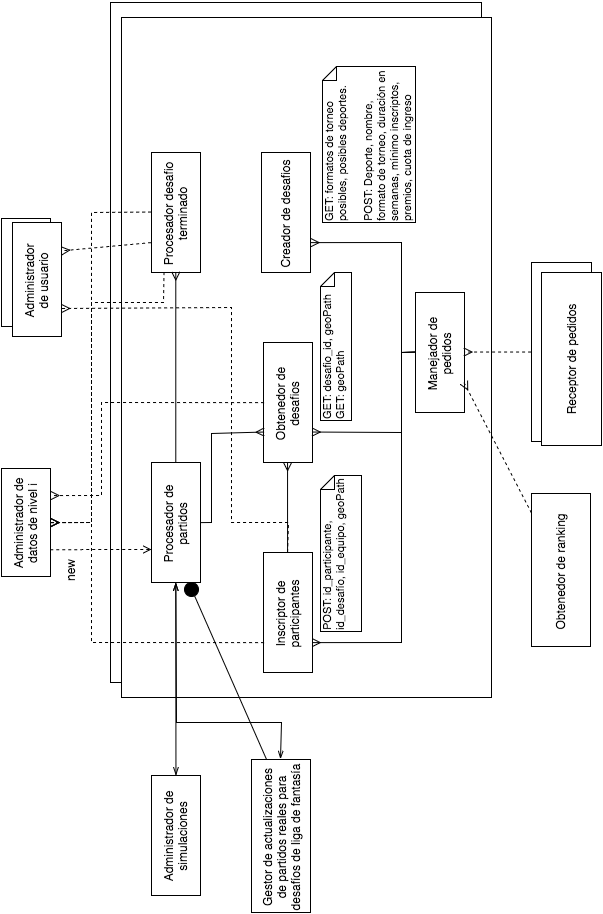
\includegraphics[height=0.95\textheight]{reentrega/imagenes/desafios-1.png}
   \caption{Zoom de Administrador de desafios.}
\end{figure}

Un administrador de desafíos se encarga de crear y mostrar desafíos, inscribir participantes y procesar (en el momento correspondiente) los partidos que componen un desafío.
Su interfaz permite:
\begin{itemize}
	\item Obtener información de un determinado desafío mediante el id_desafío y geoPath correspondiente.
	\item Obtener información de todos los desafíos abiertos de un determinado geoPath.
	\item Inscribir un participante en un desafío.
	\item Crear desafíos
	\item Ver qué tipos de desafíos es posible crear
\end{itemize}

Para entender su funcionamiento hagamos zoom en cada uno de los componentes:

% SEGUNDA FIGURA
\begin{figure}[H]
   \centering
   \includegraphics[width=\textwidth]{reentrega/imagenes/desafios-2.png}
   \caption{Zoom de Inscriptor de participantes.}
\end{figure}

Inscriptor de participantes: Dado un pedido de inscripción con id_desafio, id_usuario, equipo_id y geoPath, el procesador de solicitudes de inscripcion de desafíos llama al
obtenedor de desafios para conocer cuál es la cuota necesaria para anotarse en el desafío con id_desafio. Luego, hace un request al validador de inscripción pasándole el id_usuario, cuota
necesaria para anotarse, id_equipo y geoPath. El validador de inscripción verifica que el id_equipo sea un equipo de id_usuario y que, además, el usuario disponga de las fichas necesarias
para anotarse al desafío. Si el validador valida que la información es correcta entonces el procesador de solicitudes llama al cobrador de inscripción que fowardea el pedido al administrador de usuarios para que se descuente la cuota del usuario que se quiere inscribir. Luego, el inscriptor de usuario inscribe al usuario en el desafio llamando al administrador
de datos que persiste esta información.

% TERCER FIGURA
\begin{figure}[H]
  \centering
  \includegraphics[width=\textwidth]{reentrega/imagenes/desafios-3.png}
  \caption{Zoom Creador de desafios.}
\end{figure}

Creador de desafios: El creador de desafíos se encarga, como su nombre indica, de crear desafíos y de consultar qué tipos de desafíos se pueden crear. Para ello, utiliza el administrador de
datos.

% CUARTA FIGURA
\begin{figure}[H]
  \centering
  \includegraphics[width=\textwidth]{reentrega/imagenes/desafios-4.png}
  \caption{Zoom Obtenedor de desafíos.}
\end{figure}

Obtenedor de desafíos: el recolector de detalles de desafío devuelve el estado de un desafio especifico (o todos los del geoPath solicitado si no se especificó un desafío en particualar): si está abierto a inscripciones, si se esta jugando o si está terminado, y todos los detalles asociados: premios, cuota de inscripción, tipo de desafío, formato de torneo o fechas que se juegan, etc. El recolector de ranking obtiene el ranking para un determinado desafío.

% QUINTA FIGURA

\begin{figure}[H]
  \centering
  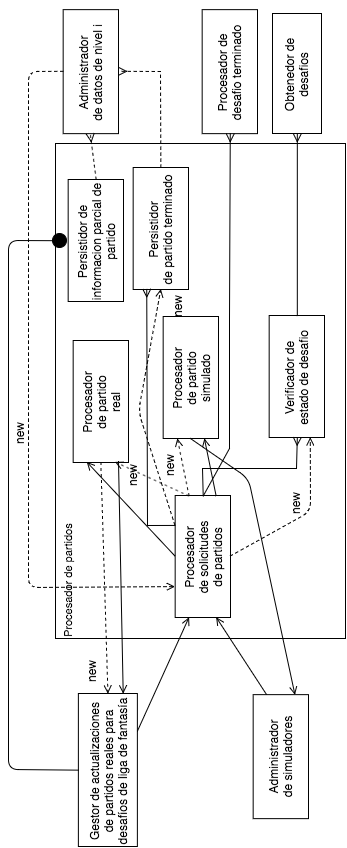
\includegraphics[height=0.95\textheight]{reentrega/imagenes/desafios-5.png}
  \caption{Zoom Procesador de partidos.}
\end{figure}

Procesador de partidos:
Flujo para el procesamiento de un partido simulado: El administrador de datos dispara un trigger al procesador de solicitudes de partidos para que este procese el partido
que acaba de comenzar. Como se trata de un partido simulado, el procesador de solicitudes llama al procesador de partido simulado. Este, le avisa el administrador de simuladores que la simulación debe comenzar. Una vez finalizada la misma, el administrador de simuladores le informa al procesador de solicitudes que el partido finalizó y cómo (quién ganó). Luego, persistidor de partido terminado persiste en el administrador de datos toda la información relacionada al partido que acaba de finalizar.
En caso de que el partido fuera el último del desafío (condición que es verificada por el Verificador de estado de desafío), se llama al procesador de desafío terminado para finalizar el desafío.
Flujo para el procesamiento de un partido real: Parecido al flujo antes mencionado pero con algunas diferencias: si el partido que se va a ejecutar se encuentra en más de un desafío solo se dispara un trigger. Queda bajo responsabilidad del procesador de partidos persisitir el resultado de dicho partido en cada desafío que tiene el partido. Además, a diferencia de la simulación, el gestor de actualizaciones de partidos reales otorga información del partido minuto a minuto por lo cual se realizan actualizaciones periódicas del partido en el administrador de datos. Una vez finalizado el encuentro, el gestor notifica al procesador de solicitudes de partidos para que persista la finalización del mismo. El flujo aquí es igual al caso simulado.

% SEXTA FIGURA
\begin{figure}[H]
  \centering
  \includegraphics[width=\textwidth]{reentrega/imagenes/desafios-6.png}
  \caption{Zoom Procesador de desafio terminado.}
\end{figure}

Procesador de desafío terminado: dado un pedido de finalizar un desafío, el receptor de desafios terminados llama al persistidor de cambio de estado de desafío para finalizar el desafío.
Luego, el entregador de premios calcula los puntos obtenidos para cada usuario y fowardea al administrador de usuarios para que persista dichos puntos.

\subsection{Administrador de Simulaciones}

% PRIMER FIGURA
% \begin{figure}[H]
%   \centering
%   \includegraphics[width=\textwidth]{imagenes/Subsistema-de-estadistica-de-partido.png}
%   \caption{Administrador de simulaciones.}
% \end{figure}

Este componente es el encargado de inicializar y correr los simuladores. En particular nos llegan pedidos del \texttt{Administrador de desafios} donde nos indican que debemos inicializar la simulación de un partido, con una referencia a que deporte es, que equipos participan y la información pertinente de los equipos, es decir jugadores y tecnico. Entonces de esta forma el Receptor de pedidos crea una nueva instancia de un Simulador, con los parametros correspondientes, deporte, equipos, jugadores, tecnico. Luego el Simulador obtiene las estadisticas de cada jugador y comienza a simular el partido, alimentandose tambien de la información recolectada de las redes sociales, para asi mejorar o empeorar el rendimiento de los jugadores.

Una vez que el \texttt{Simulador} va resolviendo la ejecución del partido, persiste en el administrador de datos el log del minuto a minuto. Asi de esta forma, en caso de que se caiga un simulador en la mitad de un partido, podemos levantar otro simulador que tome ese log parcial para seguir con el transcurso del mismo.

Una vez finalizada la simulación del partido, el \texttt{Simulador} le informa al Receptor de Pedidos el resultado del mismo, para que este se lo informe a su vez al administrador de desafios.

Por otro lado, me pueden llegar pedidos de que desean ver la simulación de algun desafio que se esta ejecutando localmente. De esta forma me llegaria un pedido del \texttt{Administrador de flujo de simulaciones} hacia el Receptor de Pedidos, donde me piden la simulacion de un partido. En caso de tratarse de un partido que todavia no estamos brindando la simulación, el \texttt{Receptor de Pedidos} crea una nueva instancia de un \texttt{Generador de Log Simulable}, una vez creada esta nueva isntancia, le notifico al \texttt{Simulador} pertinente que tiene que comenzar a mandarle el log a este nuevo Generador. Luego este Generador lo que hace es transformar el log minuto a minuto en un log mas rico, que los renders entienden para poder simularlo y mostrarlo graficamente, y enviarselo al \texttt{Administrador de flujo de simulaciones}. Luego el \texttt{Receptor de Pedidos} se guarda que ese partido ya  estamos brindando la simulación. Entonces, en caso de tratarse de un partido el cual ya estamos brindando la simulacion, no se hace nada.

Cada vez que el \texttt{Receptor de Pedidos} recibe una notificacion de fin de partido por parte del \texttt{Simulador}, elimina esta entrada de la tabla donde persiste las simulaciones que estamos brindando en estos momentos y se encarga de destruir las instancias creadas para ese partido en particular.


\subsection{Manejador de pedidos de nivel 5 + cliente}

\begin{figure}[H]
   \centering
   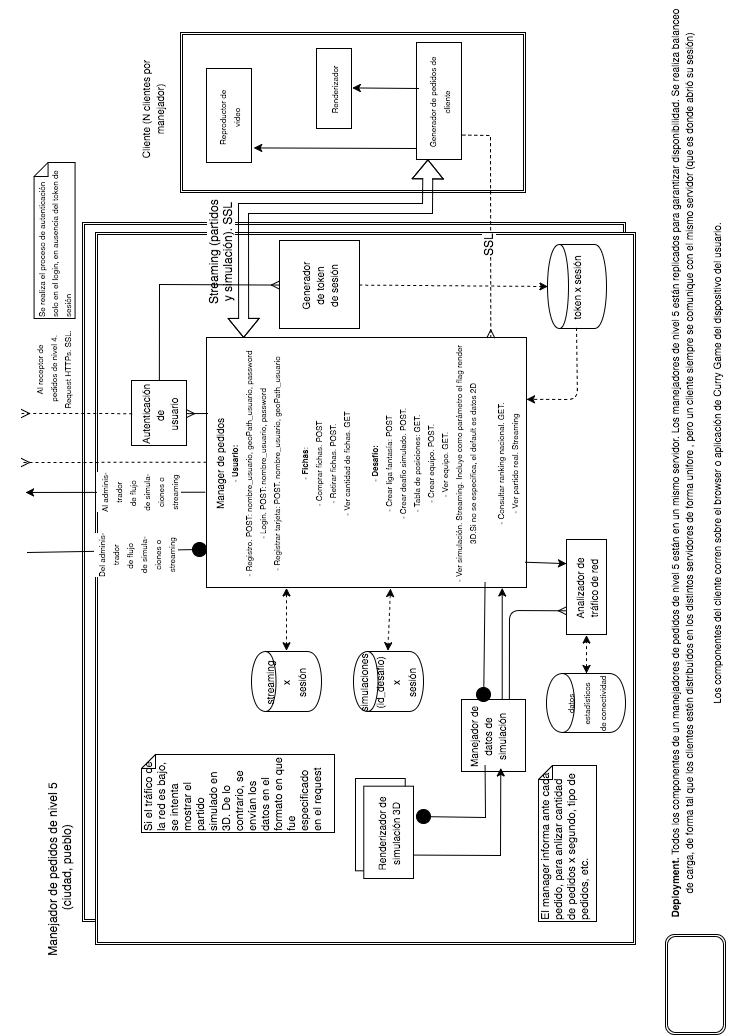
\includegraphics[height=0.95\textheight]{reentrega/imagenes/nivel-5-manejador-cliente.png}
   \caption{Manejador pedidos de nivel 5.}
\end{figure}

Toda interacción, salvo el registro, comienza con la creación de una sesión, que se utiliza tanto como mecanismo de seguridad como performance, para no autenticar al usuario por cada pedido que desea realizar.
Cada sesión está representada con un token, que se calcula durante el proceso de login.

El cliente envía usando SSL su usuario y contraseña. El manejador le forwardea el pedido al manejador de usuarios de nivel 4, y en el caso de que la autenticación sea exitosa se inicia una sesión representada por un token, que es almacenada en un repositorio. El token se envía encriptado al cliente, y en cada pedido que este haga deberá incluírlo. De esta manera, mientras la sesión no expire, el manager de pedidos verificará la existencia de una sesión abierta para dicho pedido lo cual ahorra un tiempo considerable.

Los usuarios pueden realizar distintos tipos de pedidos, enumerados en el manager de pedidos. La mayoría de ellos, con excepción del rendering de las simulaciones y el streaming de partidos se forwardean al receptor de pedidos del nivel 4.

Un pedido para ver una simulación se traduce en una suscripción al conector de 'Administrador de flujo de simulaciones', que a partir de ese momento comenzará a publicar el detalle de las simulaciones. Todas las sesiones que han solicitado ver la simulación de un determinado desafío se guardan en un repositorio. Con esto se logran 2 objetivos: Por un lado, evitar enviar suscripciones a simulaciones de desafíos de los que ya se está siendo notificado (Performance, Disponibilidad. No saturar la red). Por el otro, cuando llega un evento de la simulación de un desafío, saber qué sesiones están siguiendo dicho desafío para poder enviarles los datos.
El streaming de los partidos reales sigue un proceso análogo.

Ante cada pedido, el manager le informa al analizador de tráfico acerca de este nuevo pedido y su tipo (si es un login, consulta de ranking, pedio de streaming o simulación, etc).

Los pedidos de ver una simulación toman como parámetro el modo en que desea recibirse. Por default se asume que son datos en formato rendering de 2D (que son los que cualquier dispositivo puede reproducir). Sin embargo, un usuario puede indicar querer recibir datos de rendering 3D si su dispositivo lo soporta.

En el momento en que llegan datos de una simulación, el manejador de datos de simulación consulta al analizador acerca del estado de la red. En el caso en el que la misma no esté sobrecargada, es el mismo manejador de pedidos de nivel 5 quien renderiza en 3D los datos y los envía como video, con el objetivo de que la mayor cantidad de usuarios (sobre todo aquellos que no tienen un dispositivo poderoso para renderizar los datos 3D) puedan gozar de la simulación en su máxima calidad. Por el contrario, si la red está congestionada (por ejemplo, si muchos usuarios están viendo streaming de partidos reales o simulaciones) entonces se envían los datos sin procesar.

\subsection{Procesador de Solicitudes HTTP iniciales, geolocalización de IPs y monitoreo de servidores de nivel 5} \label{seccionDNS}

% gráfico DNS

El cliente ingresa la URL del sitio. Esto dispara una consulta DNS del navegador
que retorna aleatoriamente la IP de alguno de los servidores de nivel 1.

Luego el cliente se conecta al servidor de nivel 1 haciendo un GET de HTTP. Esto
lo recibe el $"$Receptor de solicitud global$"$, que lee la IP fuente y se la pasa al
$"$Seleccionador de servidor de nivel 5 según IP$"$. Este primero obtiene el GeoPath
usando el $"$Obtenedor de GeoPath según IP$"$ y luego busca en el repositorio de servidores
de nivel 5 todos los que estén atendiendo clientes en esa ubicación geográfica y elige uno
de ellos al azar. Luego retorna la DNS de ese servidor de nivel 5. El $"$Receptor de solicitud
global$"$ luego envía un mensaje de $"$Redirect$"$ de HTTP con la nueva DNS. Esto en el cliente
desencadena una nueva consulta DNS por la IP del servidor de nivel 5 correspondiente, y el
flujo de comunicación continúa con el cliente enviando un GET de HTTP al servidor de nivel 5.

El $"$Obtenedor de GeoPath según IP$"$ busca en el repositorio de GeoPaths por IPs. Este
repositorio está en cada uno de los servidores de nivel 1 y contiene una tabla con todos los
rangos de IP del mundo mapeados a su ubicación geográfica usando GeoPath. Este repositorio
se actualiza todos los días a las 04:00hs de la zona horaria donde el servidor se encuentra
físicamente. Para actualizarse, se consulta un servicio externo de geolocalización que indica los
cambios que hubo a nivel mundial. En el caso extremo que una IP es consultada pero aún no
está en este repositorio, el $"$Obtenedor de GeoPath según IP$"$ detectará la ausencia de la misma
y entonces ingresará el pedido en el repositorio de $"$IPs nuevas sin GeoPath$"$. Este repositorio
funciona como blackboard e inmediatamente despierta el proceso de actualización de IPs,
que consulta únicamente la IP solicitada y la escribe en el repositorio de IPs según GeoPath, para
que el otro proceso la consuma (se queda haciendo polling hasta que aparece). Se usa un
repositorio porque podría haber más de una IP nueva al mismo tiempo, y en tal caso cuando el proceso
de actualización se despierta, actualiza todas las que haya en simultáneo.

Para que este esquema funcione, debemos registrar un nombre para cada servidor de cada nivel en
el sistema DNS. Por ejemplo, si nuestro dominio fuera www.currygame.com, deberíamos registrar todas
las IPs de servidores de nivel 1 a ese nombre. Asumismos que DNS distribuye uniformemente
las consultas entre las distintas IPs (por ejemplo, siempre elige una random con distribución uniforme).
Luego cada servidor específico debe tener un nombre específico, por ejemplo:

\begin{itemize}
	\item ar.n1.s2.currygame.com - Nivel 1 de Argentina, server 2.
	\item ar.n5.s40.currygame.com - Nivel 5 de Argentina, server 40 (que podría ser uno de CABA, BsAs).
\end{itemize}

Esto permite que el cliente luego pueda ingresar directamente usando la URL específica de su región
y no necesite hacer la redirección.

\newpage

\bibliographystyle{plain}
\bibliography{tp3}

\end{document}
